%%%%%%%%%%%%%%%%%%%%%%%%%%%%%%%%%%%%%%%%%%%%%%%%%%%%%%%%%%%%%%%%%%%%%
\documentclass[letterpaper,12pt, oneside]{book}
\usepackage{TesisUTB}
\usepackage{url}
\usepackage{listings}
\usepackage{booktabs}
\usepackage{ragged2e}

% --- Numeracion de ecuaciones por capitulo (clase book: figuras/tablas ya lo hacen) ---
\counterwithin{equation}{chapter}

% --- Rotulo de tablas: "Tabla" en lugar del "Cuadro" de babel-spanish ---
% El cuerpo del texto, cleveref y la lista usan "Tabla"/"Lista de tablas", pero
% babel-spanish rotula los captions como "Cuadro N", de modo que la misma tabla
% aparecia como "Cuadro 7.11" en el caption y como "Tabla 7.11" en el parrafo
% que la cita. Se unifica el rotulo (la numeracion no cambia).
\addto\captionsspanish{\renewcommand{\tablename}{Tabla}}

% --- Referencias cruzadas uniformes (cargar despues de hyperref) ---
\usepackage[nameinlink]{cleveref}
\crefname{equation}{ecuación}{ecuaciones}
\Crefname{equation}{Ecuación}{Ecuaciones}
\crefname{figure}{figura}{figuras}
\Crefname{figure}{Figura}{Figuras}
\crefname{table}{tabla}{tablas}
\Crefname{table}{Tabla}{Tablas}
\crefname{chapter}{capítulo}{capítulos}
\Crefname{chapter}{Capítulo}{Capítulos}
\crefname{section}{sección}{secciones}
\Crefname{section}{Sección}{Secciones}

% --- Conjunciones de cleveref en español (rangos y listas) ---
% Sin esto, cleveref usa el inglés por defecto (" to ", " and "):
%   "Capítulos 8 to 10" en vez de "Capítulos 8 a 10".
% Con babel, cleveref define estas conjunciones en \AtBeginDocument,
% por lo que deben redefinirse también ahí (no en el preámbulo directo).
\AtBeginDocument{%
  \renewcommand{\crefrangeconjunction}{ a~}%
  \renewcommand{\crefpairconjunction}{ y }%
  \renewcommand{\crefmiddleconjunction}{, }%
  \renewcommand{\creflastconjunction}{ y }%
  \renewcommand{\crefpairgroupconjunction}{ y }%
  \renewcommand{\crefmiddlegroupconjunction}{, }%
  \renewcommand{\creflastgroupconjunction}{ y }%
}

\lstset{
  basicstyle=\ttfamily\scriptsize,
  breaklines=true,
  columns=fullflexible,
  frame=single,
  backgroundcolor=\color{gray!8}
}
\newcolumntype{Y}{>{\raggedright\arraybackslash}X}

% Profundidad del indice: numerar hasta subsubseccion (secnumdepth=3) pero
% listar en la Tabla de Contenido solo hasta subseccion, para no sobrecargarla.
% Nota: el paquete sectsty (v2.0.2) redefine los comandos de seccion e ignora
% tocdepth, por lo que este contador solo limita los marcadores del PDF. Para
% que la Tabla de Contenido impresa se detenga en subseccion se neutraliza el
% formateador de subsubseccion en el indice.
\setcounter{tocdepth}{2}
\makeatletter
\renewcommand{\l@subsubsection}[2]{}
\makeatother
%%%%%%%%%%%%%%%%%%%%%%%%%%%%%%%%%%%%%%%%%%%%%%%%%%%%%%%%%%%%%%%%%%%%%

%%%%%%%%%%%%%%%%%%%%%%%%%%%%%%%%%%%%%%%%%%%%%%%%%%%%%%%%%%%%%%%%%%%%
%%     PLANTILLA LATEX PARA PRESENTACION DE TRABAJOS DE GRADO     %%
%%     Formato:                                                   %%
%%         letterpaper: tamaño carta                              %%
%%         12pt       : letra de tamaño 12                        %%
%%                    : espaciado simple                          %%
%%     Autor:                                                     %%
%%          DIEGO ALBERTO GUEVARA AMAYA                           %%
%%          (guevarad@utb.edu.co)        				          %%
%%%%%%%%%%%%%%%%%%%%%%%%%%%%%%%%%%%%%%%%%%%%%%%%%%%%%%%%%%%%%%%%%%%%
%                                                                 %%
% Extensión sugerida: 80 páginas                                  %%
% Producto obligatorio: Artículo científico para revista indexada %%
%                                                                 %%
%%%%%%%%%%%%%%%%%%%%%%%%%%%%%%%%%%%%%%%%%%%%%%%%%%%%%%%%%%%%%%%%%%%%
%%%%%%%%%%%%%%%%%%%%%%%%%%%%%%%%%%%%%%%%%%%%%%%%%%%%%%%%%%%%%%%%%%%%
%%%%%%%%% MODIFICA LOS DATOS EN ESTA SECCIÓN %%%%%%%%%%%%%%%%%%%%%%%
%% para modificar la portada, pies de página y encabezados %%%%%%%%%
%%%%%%%%%%%%%%%%%%%%%%%%%%%%%%%%%%%%%%%%%%%%%%%%%%%%%%%%%%%%%%%%%%%%

\def\TITULO{\textbf{Evaluación y comparación de plugins CNI para Kubernetes:\\ un enfoque orientado a QoS, seguridad y eficiencia de recursos en entornos de microservicios}}

\def\SUBTITULO{Trabajo de grado para optar al título de Ingeniero en Telemática}

\def\AUTOR{\textbf{Duwan Estiven Sierra Guerrero \\ Holman Audrey Alba Castro}}

\def\AUTORR{{Sierra \& Alba}}

\def\DIRECTOR{Gerardo Alberto Castang Montiel}

\def\CODIRECTOR{}

\def\FACULTAD{Facultad Tecnológica}

\def\PROGRAMA{Ingeniería Telemática}

\def\LINEAINVESTIGACION{Telemática - Grupo de Investigación ORION}

\def\FECHA{Junio de 2026}

\def\UTB{UNIVERSIDAD DISTRITAL FRANCISCO JOSÉ DE CALDAS}

\def\UTBS{Universidad Distrital Francisco José de Caldas}

\def\UTBB{UDFJC}

\def\LUGAR{Bogotá, D.C. - Colombia}



\begin{document}
\frontmatter




%%%%%%%%% NO MODIFICAR EN ESTA SECCIÓN %%%%%%%%%%%%%%%%
%% para modificar la portada, ir a FormatoTesis.tex %%%
%%%%%%%%%%%%%%%%%%%%%%%%%%%%%%%%%%%%%%%%%%%%%%%%%%%%%%%
% Título del trabajo de grado
% Nombre completo del estudiante
% Nombre del director (y codirector si aplica)
% Programa de Maestría en Ingeniería
% Línea de investigación
% Universidad Tecnológica de Bolívar
% Ciudad y fecha de entrega
%%%%%%%%%%%%%%%%%%%%%%%%%%%%%%%%%%%%%%%%%%%%%%%%%%%%%%%

\begin{titlepage}
    \begin{center}
        
        \vspace*{1cm}
        
        \noindent\Large \TITULO 
        
        \vfill
        
        \textbf{\AUTOR} \\[0.5cm]
        Director \DIRECTOR \\[0.2cm]                        
        \vfill
        
        % 
\includegraphics[width=0.5\textwidth]{figures/LOGO UTB 2.png}
        
        \vfill
        \PROGRAMA \\
        \LINEAINVESTIGACION\\
        \UTBS \\
        \LUGAR \\
        \FECHA
        
    \end{center}
\end{titlepage}
\include{chaptersApa/0.1_Agradecimientos}
\chapter{Resumen}
Kubernetes no impone un plugin de red específico, lo que obliga a los
equipos a seleccionar un \emph{Container Network Interface} (CNI) sin
métricas comparativas objetivas. Esta situación conduce a
sobredimensionamiento de infraestructura (CPU/RAM) y a posturas de
seguridad incompletas. El presente trabajo construye evidencia empírica
reproducible —infraestructura como código, benchmarks automatizados y
modelo de decisión multicriterio (MCDA)— para guiar esa selección.
Se evalúan Flannel, Calico, Cilium y Antrea en un clúster K3s en alta
disponibilidad sobre DigitalOcean, midiendo \emph{throughput} TCP,
latencia de establecimiento, retransmisiones y overhead de CPU/RAM del
agente CNI, así como el impacto de políticas de red Zero Trust.
Los resultados alimentan un modelo MCDA parametrizable por perfil de
uso (Fintech/seguridad, Streaming/rendimiento e IoT/recursos limitados) y un prototipo
web que expone las recomendaciones.
Los hallazgos principales muestran que ningún plugin resultó superior
en todos los criterios: Calico alcanzó el mayor throughput TCP
(1804.40 Mbps) y la menor latencia de establecimiento, mientras Flannel
registró la menor tasa de retransmisión y huella de recursos. Se
comprobó además que Flannel ---CNI predeterminado de K3s--- acepta
NetworkPolicies en la API de Kubernetes pero no las aplica en su plano
de datos, configurando un falso positivo de seguridad, y que Cilium fue
el único plugin capaz de aplicar políticas de capa 7 (HTTP). En
coherencia con esa ausencia de dominancia, el modelo arroja una
recomendación distinta por perfil: Cilium para Fintech, Calico para
Streaming y Flannel para IoT, este último por un margen estrecho.

\vspace{1cm}
\textbf{Palabras clave:} Kubernetes, CNI, NetworkPolicy, Zero Trust, MCDA, QoS, eBPF.
\chapter{Abstract}
Kubernetes does not impose a specific network plugin, forcing teams to select a \emph{Container Network Interface} (CNI) without objective comparative metrics. This situation leads to infrastructure oversizing (CPU/RAM) and incomplete security postures. This thesis builds reproducible empirical evidence —infrastructure as code, automated benchmarks, and a multi-criteria decision analysis (MCDA) model— to guide this selection. Flannel, Calico, Cilium, and Antrea are evaluated on a high-availability K3s cluster on DigitalOcean, measuring TCP throughput, establishment latency, retransmissions, and CPU/RAM overhead of the CNI agent, as well as the impact of Zero Trust network policies. The results feed a parameterizable MCDA model by use profile (Fintech/security, Streaming/performance, and IoT/limited resources) and a web prototype that displays the recommendations.
The main findings show that no plugin proved superior across all criteria: Calico achieved the highest TCP throughput (1804.40 Mbps) and the lowest connection-establishment latency, while Flannel recorded the lowest retransmission rate and resource footprint. Flannel —the default CNI in K3s— was also found to accept NetworkPolicies through the Kubernetes API without enforcing them in its data plane, constituting a security false positive, and Cilium was the only plugin capable of enforcing layer-7 (HTTP) policies. Consistent with this absence of dominance, the model yields a different recommendation for each profile: Cilium for Fintech, Calico for Streaming, and Flannel for IoT, the latter by a narrow margin.

\vspace{1cm}
\textbf{Keywords:} Kubernetes, CNI, NetworkPolicy, Zero Trust, MCDA, QoS, eBPF.
\newpage
%\include{Abstract}
%%%%%%%%%%%%%%%%%%%%%%%%%%%%%%%%%%%%%%%%%%%%%%%%%%%%%%%%%%%%%%%%%%%%%

\tableofcontents
\addcontentsline{toc}{chapter}{Tabla de Contenido}

\renewcommand{\listtablename}{Lista de tablas}
\listoftables
\addcontentsline{toc}{chapter}{Lista de tablas}

\listoffigures
\addcontentsline{toc}{chapter}{Lista de figuras}

\cleardoublepage
\mainmatter

%%%%%%%%%%%%%%%%%%%%%%%%%%%%%%%%%%%%%%%%%%%%%%%%%%%%%%%%%%%%%%%%%%%%%
% --- Parte I: Fundamentación ---
% Nota: Planteamiento del problema, Justificación y Objetivos se integraron
% como secciones dentro de 1_Introduccion (archivos 3/4/5 conservados sin incluir).
\chapter{Introducción} \label{sec:Introduccion}

\section{Contexto y motivación}

La adopción de Kubernetes como plataforma de orquestación de contenedores se ha consolidado en la industria tecnológica, pero su viabilidad operativa depende en gran medida del componente de red que conecta los servicios dentro del clúster. Kubernetes no incluye por defecto un mecanismo de conectividad entre contenedores: delega esa función en un complemento intercambiable denominado Container Network Interface (CNI), cuya selección recae en el equipo técnico de cada organización.

Los equipos deben escoger entre múltiples complementos ---Calico, Cilium, Flannel y Antrea, entre otros--- sin contar con criterios de comparación objetivos ni datos de rendimiento medidos en condiciones representativas. Esta carencia conduce a tres problemas interrelacionados: configuraciones de red inseguras por la elección de complementos que no aplican políticas de control de acceso en su plano de datos, sobredimensionamiento de recursos computacionales por desconocimiento del costo real de cada complemento en CPU y memoria, y una exposición silenciosa a vulnerabilidades que el equipo operativo no detecta hasta que afectan a los usuarios.

La pregunta de investigación que motiva este trabajo es la siguiente: ¿cómo pueden las organizaciones comparar complementos de red y automatizar políticas de comunicación segura para optimizar recursos sin degradar el rendimiento?

De esta pregunta principal se derivan cuatro sub-preguntas específicas que estructuran la evaluación empírica:

\begin{enumerate}
    \item ¿Cuáles son las diferencias en velocidad de respuesta ---throughput, latencia y retransmisiones TCP--- entre los plugins CNI evaluados bajo condiciones controladas de carga?
    \item ¿Cómo impacta cada CNI en el consumo de recursos del nodo ---CPU y memoria RAM--- durante sesiones de red de alta intensidad?
    \item ¿Qué tan efectivo es cada CNI para aplicar Network Policies de seguridad, y cuál es el overhead que introduce sobre el rendimiento?
    \item ¿En qué medida la diferencia de eficiencia entre plugins permite reducir el sobredimensionamiento de infraestructura a escala de clúster?
\end{enumerate}

La evaluación empírica de complementos de red permite fundamentar esas decisiones con datos medidos, no con suposiciones. Este trabajo proporciona esa evidencia para cuatro CNIs representativos, junto con una metodología replicable por cualquier equipo que necesite realizar la misma comparación. Para operacionalizar esta evaluación, el proyecto provee dos entregables técnicos principales: un banco de pruebas de red (testbed) reproducible mediante infraestructura como código (IaC) para la obtención automática de métricas, y una herramienta interactiva recomendadora en formato de aplicación web de página única (SPA). Estos componentes traducen los datos empíricos recopilados del plano de datos en decisiones estructuradas de configuración y dimensionamiento para las organizaciones.

\section{Planteamiento del problema} \label{sec:Planteamiento}

Kubernetes se ha convertido en el estándar de facto para desplegar aplicaciones modernas en contenedores, pero el rendimiento, la seguridad y la eficiencia de un clúster no dependen solo del orquestador. Dependen del complemento de red que conecta los servicios entre sí. Esta responsabilidad recae en los plugins CNI, que determinan cómo se enrutan los paquetes, qué tan rápido viajan y qué comunicaciones están permitidas o bloqueadas.

El problema es que no existe un criterio objetivo y ampliamente adoptado para elegir entre los distintos CNIs disponibles. Las decisiones de selección suelen apoyarse en documentación dispersa, recomendaciones informales o en el plugin configurado por defecto ---en el caso de K3s, Flannel---, sin datos de rendimiento medidos en condiciones representativas. El resultado concreto es triple: configuraciones de red inseguras, porque algunos complementos no aplican en el tráfico real las políticas que el operador cree activas; clústeres sobredimensionados, porque sin conocer el costo real de CPU y RAM de cada CNI se agregan recursos a modo de margen de seguridad; y fallos que solo se detectan cuando ya afectan al usuario final, porque la red interna del clúster carece de observabilidad.

El problema se agrava porque Kubernetes provee los mecanismos necesarios ---NetworkPolicies, autoescalado, observabilidad---, pero su aplicación efectiva requiere conocimientos especializados y pruebas sistemáticas que la mayoría de equipos no tiene capacidad de realizar. En entornos donde la disponibilidad es crítica, operar sobre supuestos en lugar de evidencias convierte la red en el punto débil del sistema.

Esta investigación parte de la necesidad de comparar CNIs con datos objetivos y de automatizar la validación de políticas de red, para que las organizaciones puedan garantizar seguridad, rendimiento y eficiencia sin incrementar la complejidad operativa. Para resolver esta brecha, el proyecto propone dos entregables técnicos: un banco de pruebas de red (testbed) reproducible basado en infraestructura como código (IaC) para la recolección automática de telemetría y una aplicación web interactiva (SPA) que implementa el algoritmo MCDA. Estos instrumentos reducen la complejidad operativa al traducir las mediciones del plano de datos en decisiones de configuración directa y dimensionamiento correcto de recursos.

\section{Justificación} \label{sec:Justificacion}

La adopción de Kubernetes como estándar de facto para el despliegue de aplicaciones en contenedores ha trasladado una decisión crítica al equipo técnico de cada organización: la selección del complemento de red (CNI) que conecta los servicios dentro del clúster. Esta decisión es de naturaleza telemática ---determina cómo se enrutan los paquetes, con qué latencia y throughput viajan, qué comunicaciones se permiten y cuántos recursos consume el plano de red---, pero en la práctica se toma sin evidencia medida, apoyándose en documentación dispersa o en el complemento configurado por defecto~\cite{ref29}. Este trabajo se justifica precisamente por esa brecha: convierte una elección basada en intuición en una decisión fundamentada en datos reproducibles.

\subsection{Pertinencia telemática}

El aporte se ubica en el núcleo de la ingeniería telemática: la convergencia entre redes de datos y servicios distribuidos. Tres dimensiones telemáticas estructuran la solución. La primera es la \textbf{Calidad de Servicio (QoS)}: la medición controlada de throughput, latencia de establecimiento y retransmisiones TCP entre nodos cuantifica el comportamiento real de la red del clúster bajo carga. La segunda es la \textbf{observabilidad de red}: la instrumentación con Prometheus y Grafana sobre el agente CNI hace visible el tráfico este-oeste interno, un plano que las herramientas tradicionales de monitoreo no cubren. La tercera es la \textbf{micro-segmentación bajo Zero Trust}: la automatización y validación de NetworkPolicies traduce el principio de mínimo privilegio en reglas verificables sobre el plano de datos. En conjunto, el proyecto no evalúa un producto de software genérico, sino el comportamiento telemático de la infraestructura de comunicaciones de un clúster.

\subsection{Impacto en las organizaciones}

El beneficio para las organizaciones que sigan esta guía de implementación es directo y medible. Conocer el costo real en CPU y memoria de cada CNI por unidad de tráfico permite dimensionar la infraestructura con base en evidencia y reducir el \emph{sobredimensionamiento preventivo} ---la práctica de adquirir capacidad ``por si acaso'' que genera gasto innecesario en infraestructura y energía~\cite{ref7,ref8}. La validación automatizada de políticas de red cierra brechas de seguridad que suelen permanecer ocultas hasta que un incidente las revela, sin elevar la complejidad operativa. Y la entrega de un método replicable ---infraestructura como código, \emph{benchmarks} automatizados y un modelo de decisión---  permite que equipos sin especialización profunda en redes de Kubernetes realicen la misma comparación en su propio entorno. El impacto se resume en tres ejes: decisiones de arquitectura basadas en datos, reducción de costos operativos y una postura de seguridad verificable.

\subsection{Aporte académico y entregables}

Frente a los estudios comparativos existentes, que suelen reportar mediciones aisladas de rendimiento, este trabajo integra la evaluación de QoS, la seguridad y la eficiencia de recursos en un único modelo de decisión multicriterio parametrizable por perfil de uso. El resultado tangible no es solo el documento, sino una \textbf{herramienta}: un testbed reproducible y un prototipo recomendador que expone, para cada perfil organizacional, qué CNI conviene y por qué. Esta orientación hacia un producto verificable ---y no únicamente hacia un informe--- es coherente con la modalidad de monografía orientada a la solución de un problema tecnológico mediante modelos, prototipos y productos~\cite{ref29}.

\subsection{Viabilidad}

El proyecto es viable técnica, económica y legalmente. La totalidad del \emph{stack} ---Kubernetes (K3s), Calico, Cilium, Flannel, Antrea, Prometheus, Grafana, iperf3--- se distribuye bajo licencias permisivas (Apache~2.0, MIT, BSD o GPL) que habilitan su uso académico sin restricciones. La infraestructura se aprovisiona bajo demanda en la nube pública con un costo acotado y controlado mediante automatización, y no se manipulan datos personales ni información sensible, por lo que no aplican consideraciones de protección de datos.

\section{Objetivos} \label{sec:Objetivos}

\subsection{Objetivo General}

Desarrollar un modelo de evaluación, selección y validación de plugins CNI en Kubernetes, compuesto por una guía metodológica, un prototipo de pruebas de laboratorio y una lista de verificación.

\subsection{Objetivos Específicos}

\begin{enumerate}
  \item Evaluar cuantitativamente el rendimiento de los CNI disponibles para Kubernetes (Calico, Cilium, Flannel y Antrea) mediante pruebas controladas de latencia, velocidad de transferencia y uso de recursos, para identificar sus fortalezas y limitaciones en escenarios reales.
  \item Evaluar cómo la configuración segura y automatizada de las políticas de red adaptadas a cada plugin CNI reduce la superficie de ataque y la probabilidad de incidentes de seguridad en clústeres Kubernetes, con el fin de determinar su capacidad de reducir vulnerabilidades y prevenir incidentes de seguridad en entornos de laboratorio representativos de producción.
  \item Desarrollar, como parte del modelo propuesto, un conjunto de criterios y métricas que permitan la comparación objetiva entre diferentes CNI para Kubernetes mediante la definición de umbrales de rendimiento y factores de ponderación, para facilitar la toma de decisiones técnicas basadas en evidencia cuantificable.
  \item Implementar un prototipo funcional que recomiende y configure el CNI más adecuado según las necesidades específicas de cada organización, para simplificar el proceso de implementación y apoyar la definición de configuraciones recomendadas en entornos de prueba.
\end{enumerate}

\section{Alcance del trabajo}

Esta tesis tiene como objetivo desarrollar un modelo de evaluación, selección y validación de complementos CNI en clústeres Kubernetes. El trabajo evalúa Flannel, Calico, Cilium y Antrea en un clúster K3s hospedado en la nube de DigitalOcean, midiendo la velocidad de transferencia, la latencia, el uso de CPU, de memoria y la efectividad de las políticas de seguridad. No obstante, esta investigación solo considera configuraciones de red superpuestas (overlay). El estudio excluye despliegues en servidores físicos (bare-metal) o enrutamiento nativo debido a las restricciones de la red virtual privada.

\section{Estructura del documento}

Este capítulo introductorio ha presentado el contexto y la motivación, el planteamiento del problema, la justificación, los objetivos y el alcance del trabajo. El \cref{cap:marco_teorico} desarrolla el marco teórico-conceptual y el \cref{sec:EstadoArte} revisa la literatura sobre la evaluación de CNIs, la seguridad Zero Trust y los modelos de decisión. Los \cref{cap:metodologia,sec:Metodos,cap:herramienta} detallan la metodología de trabajo, el diseño de la solución y su implementación y despliegue. Finalmente, los \cref{sec:Resultados,sec:Discusion,sec:Conclusiones,sec:Recomendaciones,sec:TrabajosFuturos} documentan los resultados experimentales, la discusión de implicaciones, las conclusiones, las recomendaciones y el trabajo futuro.

% --- Parte II: Marco de referencia ---
\chapter{Marco Teórico - Conceptual} \label{cap:marco_teorico}

\section{El modelo de red de Kubernetes}

Kubernetes (K8S) no implementa por sí mismo la conectividad entre cargas de trabajo; define un modelo de red y delega su realización en componentes externos. Comprender este modelo es necesario para interpretar las métricas del experimento, dado que el plano de red ---y en particular el plugin que lo implementa--- determina el rendimiento, la seguridad y la eficiencia en la utilización de recursos dentro del clúster~\cite{ref2}.

El modelo de red de Kubernetes establece tres principios fundamentales:
\begin{enumerate}
    \item Cada Pod recibe una dirección de Protocolo de Internet (IP, Internet Protocol) propia y única.
    \item Los Pods se comunican entre sí sin traducción de direcciones de red (NAT, Network Address Translation).
    \item Los agentes del host (como kubelet) alcanzan a todos los Pods ubicados en ese nodo.
\end{enumerate}
Sobre estas garantías se construyen las abstracciones de descubrimiento, balanceo y control de acceso del clúster~\cite{ref2}.

La siguiente analogía ayuda a visualizar cómo interactúan estos componentes:
\begin{itemize}
    \item \textbf{Pods (Viviendas):} Constituyen las residencias particulares del clúster. Cada Pod cuenta con una dirección IP única y efímera que le permite comunicarse directamente con cualquier otra vivienda del entorno sin intermediarios.
    \item \textbf{Nodos (Barrios):} Alojan múltiples viviendas y proveen los recursos físicos y de cómputo (CPU, memoria y conectividad) indispensables para la subsistencia de los servicios.
    \item \textbf{Servicios (Central telefónica):} Operan como un conmutador estable con un número de contacto único e invariable. Esto permite canalizar el tráfico hacia las réplicas adecuadas, independientemente de los cambios internos en su ciclo de vida.
    \item \textbf{Ingress y Gateway API (Portería):} Representan el acceso administrado y seguro desde el exterior (Internet), asegurando el gobierno del tráfico entrante y la separación de responsabilidades funcionales.
\end{itemize}

El sustrato vial que hace posible la comunicación física entre las viviendas y barrios corresponde a la Interfaz de Red de Contenedores (CNI, Container Network Interface), la cual se detalla en la Figura~\ref{fig:red_cluster_k8s} y define la infraestructura de red subyacente.

\begin{figure}[htbp]
    \centering
    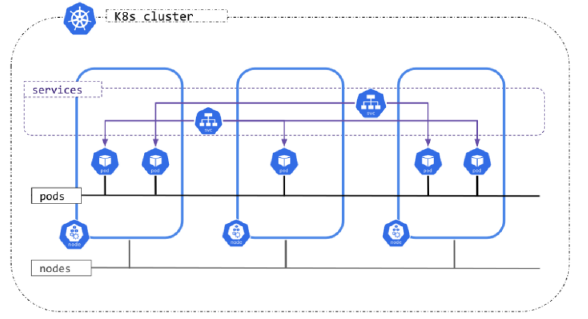
\includegraphics[width=0.85\textwidth]{figures/red_cluster_k8s.png}
    \caption{Topología de red de un clúster de Kubernetes (adaptado de~\cite{ref2}).}
    \label{fig:red_cluster_k8s}
\end{figure}

\subsection{Identidad de red del Pod}

Kubernetes adopta el modelo de direccionamiento IP por Pod, asignando una dirección única a cada unidad de ejecución. Este enfoque facilita que las cargas de trabajo interactúen de forma directa y nativa sin recurrir a NAT. Dado que la identidad del Pod es efímera ---las réplicas se crean, destruyen y sustituyen de manera dinámica por los controladores---, la plataforma requiere abstracciones estables para asegurar el descubrimiento y direccionamiento consistente de los destinos~\cite{ref2}.

\subsection{Nodos y reenvío de paquetes}

Cada nodo (Host o máquina virtual/física) hospeda múltiples Pods y aporta recursos de CPU, memoria y conectividad. En este nivel se instalan las rutas del sistema operativo y los mecanismos de reenvío local que garantizan la entrega de paquetes al Pod de destino, conforme al modelo de red del clúster: alcance directo entre Pods, ausencia de superposición de rangos de red y conectividad bidireccional este-oeste~\cite{ref2}. El agente del plugin de red se ejecuta precisamente en este nivel; por ello, su consumo de CPU y memoria por nodo Worker constituye una de las métricas centrales de la comparativa.

\subsection{Direccionamiento estable: Services y EndpointSlices}

Un Service expone un identificador estable ---una dirección IP virtual (VIP, Virtual IP) conocida como ClusterIP--- que representa a un conjunto de Pods equivalentes. El cliente se conecta a esa IP virtual y la plataforma balancea la solicitud hacia una de las réplicas disponibles, desacoplando a los consumidores de los cambios en el ciclo de vida de los Pods~\cite{ref3,ref13}. 

Para mantener actualizada la relación de destinos, Kubernetes emplea \emph{EndpointSlices}, los cuales mantienen un inventario actualizado de las direcciones IP y puertos de los Pods que respaldan cada Service. Este mecanismo reduce significativamente la sobrecarga de control frente a los antiguos Endpoint monolíticos en clústeres de gran escala~\cite{ref1}. Esta capa es relevante para interpretar la latencia medida: el tiempo en que una solicitud alcanza el Pod correcto comprende tanto la resolución del balanceador (iptables, IPVS o eBPF) como el reenvío realizado por el plugin de red.

\subsection{Ingreso de tráfico externo: Ingress y Gateway API}

El tráfico procedente de Internet no accede directamente a los Pods, sino a través de una capa de ingreso administrada. La \emph{Gateway API} formaliza los roles asociados ---infraestructura, operaciones y desarrollo--- y las reglas de capa 7 (como hostnames, rutas y terminación TLS) que determinan el enrutamiento de cada solicitud hacia el Service correspondiente~\cite{ref17}. 

En despliegues de alta disponibilidad, esta capa suele estar precedida por un balanceador de carga externo de capa 3/4 que distribuye el tráfico antes de que alcance los nodos del clúster~\cite{ref5}.

\subsection{Aislamiento lógico: Namespaces y NetworkPolicies}

Un \emph{Namespace} representa una delimitación lógica dentro del plano de control, orientada a organizar y estructurar recursos por proyectos, equipos o entornos (como desarrollo, pruebas y producción)~\cite{ref2}. Esta separación garantiza la unicidad de nombres DNS internos en la forma \texttt{<servicio>.<namespace>.svc.cluster.local}, lo cual previene ambigüedades en la resolución de nombres~\cite{ref13,ref2}.

Sin embargo, los Namespaces no restringen la comunicación física de red por defecto. La conectividad este-oeste permanece abierta a menos que se definan reglas explícitas de control de acceso mediante NetworkPolicies, aplicando principios de Confianza Cero (\emph{Zero Trust}) para limitar el tráfico exclusivamente a lo autorizado~\cite{ref4,ref24,ref25,ref26}.

Las NetworkPolicies funcionan como firewalls lógicos distribuidos de capa 3/4 que permiten o restringen conexiones basándose en selectores de etiquetas (\emph{labels}), puertos y protocolos, como se ilustra en la Figura~\ref{fig:network_policy}.

\begin{figure}[htbp]
    \centering
    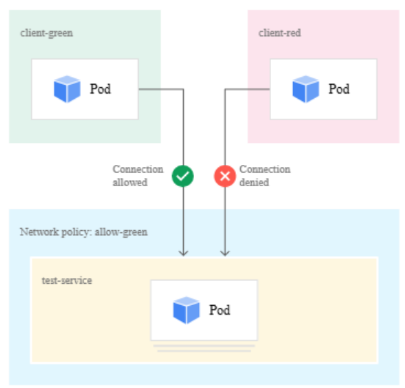
\includegraphics[width=0.85\textwidth]{figures/network_policy.png}
    \caption{Representación de política de red en Kubernetes (NetworkPolicy) con control de conexiones permitidas y denegadas. Fuente: elaboración propia.}
    \label{fig:network_policy}
\end{figure}

Su aplicación efectiva depende de que el CNI implemente el plano de control y de datos correspondiente. Si el plugin CNI seleccionado carece de soporte para NetworkPolicies, la API de Kubernetes aceptará el recurso, pero no se aplicará ninguna regla de seguridad en los nodos, dejando el clúster expuesto~\cite{ref4,ref18}.

\subsection{Recorrido de una solicitud}

El ciclo completo del tráfico responde a la siguiente secuencia operativa:
\begin{enumerate}
    \item El cliente externo envía una solicitud que llega al balanceador y se dirige a la portería lógica (Ingress o Gateway API)~\cite{ref17}.
    \item La portería inspecciona el paquete en capa 7 y lo reenvía al Service adecuado~\cite{ref3,ref13}.
    \item El Service distribuye la petición consultando los EndpointSlices activos para elegir un Pod de destino~\cite{ref1}.
    \item El plugin de red encamina el tráfico hasta el Pod de destino en su nodo correspondiente~\cite{ref2,ref4,ref18}.
\end{enumerate}

\section{La Interfaz de Red de Contenedores (CNI)}

\subsection{Especificación y funciones núcleo}

La especificación Container Network Interface (CNI) define el estándar mediante el cual el runtime de contenedores interactúa con diversos plugins para automatizar la configuración de red. La especificación se fundamenta en operaciones simples y encadenables como la adición (\texttt{ADD}) y la eliminación (\texttt{DEL}) de interfaces de red de los contenedores~\cite{ref18,ref20,ref21,ref28}, un proceso ilustrado esquemáticamente en la Figura~\ref{fig:workflow_cni}.

\begin{figure}[htbp]
    \centering
    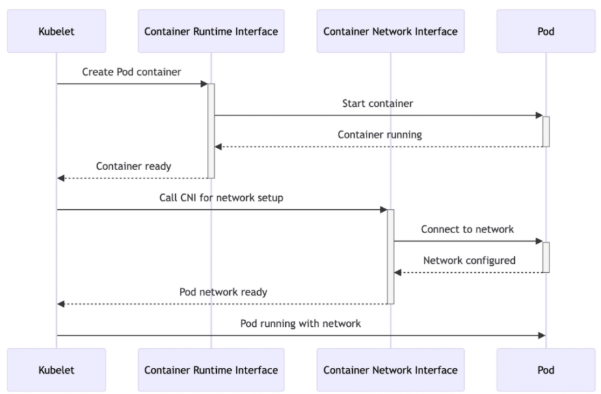
\includegraphics[width=0.85\textwidth]{figures/workflow_cni.png}
    \caption{Diagrama de operación del CNI: interacciones entre Kubelet, Pod y plugins de red.}
    \label{fig:workflow_cni}
\end{figure}

Las funciones básicas que implementa cualquier plugin CNI son:
\begin{itemize}
    \item \textbf{Identidad de Red:} Asignación de IPs del clúster que viabilizan el modelo IP-por-Pod y aseguran la comunicación este-oeste~\cite{ref2}.
    \item \textbf{Enlace e Interfaces:} Creación de veth-pairs para conectar el espacio de nombres de red (\emph{network namespace}) del Pod con la pila de red del host~\cite{ref4,ref18}.
    \item \textbf{Gestión de Direcciones (IPAM):} Reserva y liberación sistemática de direcciones de red a través de componentes como host-local~\cite{ref18,ref20}.
\end{itemize}

\subsection{Modelos de dataplane: redes superpuestas (Overlay) vs. enrutamiento nativo}

El plano de datos del CNI se suele clasificar en dos estrategias principales:
\begin{itemize}
    \item \textbf{Redes Superpuestas (Overlay):} Encapsulan los paquetes de los Pods dentro de protocolos de transporte como VXLAN o Geneve sobre UDP. Esto permite aislar el direccionamiento del clúster de la infraestructura física. Su principal ventaja radica en la simplicidad operativa y el desacoplamiento; a cambio, introduce cabeceras adicionales, posibles ajustes de MTU y cierta carga de CPU por encapsulación/descapsulación.
    \item \textbf{Enrutamiento Nativo (Directo):} Prescinde de túneles lógicos y expone las IPs de los Pods directamente a la red física mediante enrutamiento L3 convencional. Aunque mejora el rendimiento de red y reduce el consumo de CPU, demanda un diseño de direccionamiento rígido y una estrecha integración con la red corporativa.
\end{itemize}

Estudios previos muestran diferencias significativas en el desempeño según el dataplane adoptado, condicionando la viabilidad técnica en entornos con recursos limitados como edge computing o nubes públicas~\cite{ref7,ref8}. En contraste, la aceleración mediante planos de datos avanzados como Open vSwitch (OVS) o programas eBPF (extended Berkeley Packet Filter) incide sustancialmente en la latencia de procesamiento~\cite{ref11,ref22}.

\subsection{Gestión de direcciones (IPAM)}

La gestión de direcciones (IPAM) asigna y libera las IPs de los Pods de forma sistemática; una administración eficiente evita colisiones de red, habilita despliegues dual-stack y sostiene la escalabilidad ante la creación o destrucción masiva de réplicas~\cite{ref18,ref20}.

\subsection{MTU y fragmentación en redes con encapsulación}

En redes superpuestas, el overhead de la encapsulación disminuye el tamaño máximo de segmento de datos útil. Se debe ajustar la Unidad Máxima de Transmisión (MTU, Maximum Transmission Unit) efectiva restando el tamaño de las cabeceras adicionales para prevenir la fragmentación de paquetes, caídas de rendimiento y pérdidas de conexión bajo carga~\cite{ref12}, un proceso ilustrado en la Figura~\ref{fig:ajuste_mtu}.

\begin{figure}[htbp]
    \centering
    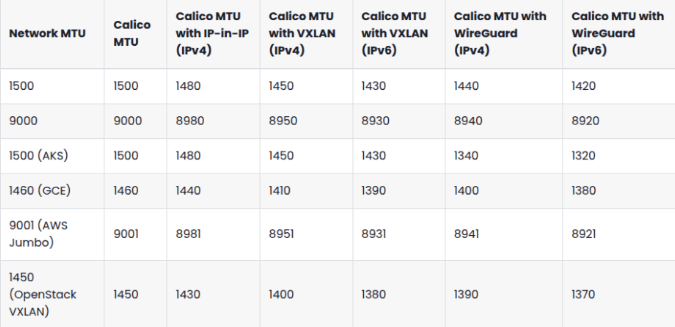
\includegraphics[width=0.85\textwidth]{figures/ajuste_mtu.png}
    \caption{Ajuste de MTU en presencia de encapsulación (p. ej., VXLAN) para evitar fragmentación y pérdida de rendimiento~\cite{ref12}.}
    \label{fig:ajuste_mtu}
\end{figure}

\subsection{Observabilidad del plano de datos}

La operación confiable de microservicios exige visibilidad sobre los flujos de red. Cuando el CNI integra monitoreo de flujos, la telemetría de origen y destino se correlaciona con las identidades nativas del clúster (Namespaces y etiquetas); así, la observabilidad de red se convierte en un componente telemático de primer orden para diagnosticar la calidad de servicio y sustentar las decisiones de configuración~\cite{ref6,ref23}.

\subsection{Métricas de rendimiento y sobredimensionamiento}

La comparación entre CNIs descansa en tres métricas principales: la latencia media y de percentiles críticos (P95 y P99), el throughput TCP/UDP sostenido y el uso de recursos (CPU y RAM) por paquete procesado~\cite{ref7,ref8}. Estas mediciones son determinantes para mitigar el sobredimensionamiento preventivo de hardware en la nube, optimizando la relación costo-rendimiento de la infraestructura~\cite{ref7,ref8,ref12,ref23,ref24,ref25}.

\section{eBPF como mecanismo de aceleración en el kernel}

El filtro de paquetes de Berkeley extendido (eBPF, \emph{extended Berkeley Packet Filter}) es una tecnología del kernel de Linux que permite ejecutar programas de forma segura dentro del propio kernel, sin modificar su código fuente ni cargar módulos adicionales~\cite{ref27}. Concebido para el filtrado de paquetes, hoy sustenta funcionalidades de red, seguridad y observabilidad dentro del sistema operativo.

Para entender por qué eBPF importa en este contexto, conviene compararlo con iptables, el mecanismo tradicional de filtrado de paquetes en Linux. iptables funciona como una lista de reglas que el kernel revisa una por una cada vez que llega un paquete: cuantas más reglas haya ---producto de más servicios y más políticas de red---, mayor es el tiempo que tarda cada decisión de enrutamiento. eBPF reemplaza ese mecanismo por tablas hash donde la respuesta se obtiene en tiempo constante, sin importar cuántas reglas existan. En un clúster con cientos de servicios y políticas de seguridad, esta diferencia se traduce en latencias medibles.

Antes de ejecutarse, cada programa eBPF es verificado por el kernel para garantizar que no comprometa su estabilidad, lo que permite extender el procesamiento de red directamente en el kernel sin los riesgos ni el sobrecosto de un módulo tradicional~\cite{ref27}.

En el contexto de los CNI evaluados en este trabajo, Cilium utiliza eBPF tanto para el reenvío de paquetes entre Pods como para la aplicación de NetworkPolicies, incluidas reglas de capa 7 sobre el protocolo HTTP. Calico también ofrece un modo eBPF opcional como alternativa a su dataplane basado en iptables~\cite{ref10}.

\section{Arquitectura de Confianza Cero y control de red en Kubernetes}

La Arquitectura de Confianza Cero (Zero Trust Architecture, ZTA) es un modelo de seguridad que parte de una premisa opuesta al perímetro de red tradicional: ninguna carga de trabajo es confiable por defecto, independientemente de si se encuentra dentro o fuera de la red corporativa. Rose et al.~\cite{ref24} formalizaron este paradigma en el NIST SP 800-207, definiendo tres principios operativos fundamentales: verificar siempre la identidad del solicitante, aplicar el menor privilegio posible en cada acceso, y asumir que la red puede estar comprometida en cualquier momento.

Una forma de imaginar Zero Trust es pensar en un edificio donde todas las puertas están cerradas con llave por defecto. Para que alguien entre a una oficina no basta con que esté dentro del edificio; necesita una llave específica para esa puerta. En Kubernetes, cada llave es una regla de NetworkPolicy.

Llevado al entorno de Kubernetes, Zero Trust se operacionaliza mediante NetworkPolicies: reglas declarativas que el CNI aplica en el plano de datos de cada nodo. El punto de partida es una política de \emph{Default Deny} ---denegar todo el tráfico por defecto--- sobre la cual se habilitan únicamente las comunicaciones explícitamente necesarias. Esta estrategia reduce la superficie de ataque porque, ante el compromiso de un Pod, el atacante no puede alcanzar otros servicios del clúster sin una regla que lo permita~\cite{ref24,ref25}.

Un aspecto crítico, y directamente relevante para este trabajo, es que la NetworkPolicy es un objeto de la API de Kubernetes, pero su aplicación efectiva depende del CNI. Si el plugin no implementa las políticas en su plano de datos, el objeto existe en la base de datos del clúster y el operador puede creerlo activo, pero no produce ningún efecto real sobre el tráfico~\cite{ref4}. Esta distinción entre la declaración de una política y su \emph{enforcement} efectivo es una de las variables centrales del experimento.

\section{Análisis de Decisión Multicriterio (MCDA)}

El Análisis de Decisión Multicriterio (MCDA) es un conjunto de métodos formales para seleccionar entre alternativas cuando existen múltiples criterios de evaluación con distinta importancia relativa~\cite{ref34}. Es el enfoque adecuado cuando ninguna alternativa es la mejor en todas las dimensiones al mismo tiempo: en este trabajo, ningún CNI lidera simultáneamente en throughput, latencia, consumo de CPU, consumo de RAM y capacidades de seguridad. Ignorar ese compromiso y elegir únicamente por throughput equivale a comprar un automóvil mirando solo la velocidad máxima.

El modelo implementado en este trabajo utiliza el método de \textbf{suma ponderada} ---conocido en la literatura como \emph{Simple Additive Weighting} (SAW) o \emph{Weighted Sum Model} (WSM)---, formalizado por Fishburn como agregación aditiva de utilidades~\cite{ref30} y reconocido como el método MCDA más difundido por su transparencia interpretativa~\cite{ref34}. La puntuación de cada alternativa se obtiene mediante la \cref{eq:mcda-suma}:
\begin{equation}\label{eq:mcda-suma}
P_{CNI} = \sum_{i=1}^{n} (V_i \times W_i)
\end{equation}
donde $P_{CNI}$ es el puntaje final del plugin CNI, $V_i$ es el valor normalizado de la métrica $i$ y $W_i$ es el peso asignado a esa métrica según el perfil de usuario evaluado, con la condición $\sum_{i=1}^{n} W_i = 1$.

Para que métricas con unidades distintas (Gbps, milisegundos, millicores) sean comparables en esa fórmula, se aplica \textbf{normalización min-max}, una de las técnicas estándar de normalización en MCDA por preservar las distancias relativas entre alternativas~\cite{ref35}. En este trabajo se re-escala al intervalo $[1,\,5]$ mediante la \cref{eq:mcda-norm}:
\begin{equation}\label{eq:mcda-norm}
V_i = 1 + 4 \cdot \frac{x - x_{\min}}{x_{\max} - x_{\min}}
\end{equation}
donde $x_{\min}$ y $x_{\max}$ son los valores mínimo y máximo observados entre los CNIs para esa métrica. En métricas donde un valor mayor es mejor (throughput), la normalización es directa; en métricas donde un valor menor es mejor (latencia, CPU, RAM), se invierte el cociente ---usando $x_{\max} - x$ en el numerador--- de modo que $V_i = 5$ representa siempre la mejor alternativa y $V_i = 1$ la peor. La elección del intervalo $[1,\,5]$ ---en lugar del clásico $[0,\,1]$--- responde a una escala de utilidad acotada de cinco niveles, equivalente a una escala Likert, que facilita la lectura por parte de equipos no especializados sin alterar el ordenamiento de las alternativas~\cite{ref35}. Con $\sum_{i=1}^{n} W_i = 1$, el puntaje $P_{CNI}$ también queda en $[1,\,5]$, lo que permite interpretar el resultado final en la misma escala.

Los pesos $W_i$ son los parámetros que capturan las prioridades de cada organización. En este trabajo se definen tres perfiles: Fintech, que asigna mayor peso a la seguridad; Streaming, orientado al rendimiento de red; e IoT, centrado en el menor consumo de recursos por nodo. La parametrización explícita de los pesos hace que el modelo sea ajustable ante nuevos perfiles sin modificar el procedimiento de medición.

El método SAW es \emph{compensatorio}: un valor alto en una métrica puede compensar un valor bajo en otra. Para impedir que esa compensación opere sobre la seguridad ---de modo que un CNI sin soporte de NetworkPolicies obtenga un buen puntaje únicamente por su eficiencia computacional---, el modelo incorpora una \textbf{restricción no compensatoria}, en la línea de los modelos conjuntivos de decisión multiatributo~\cite{ref31}. Cuando el perfil exige un nivel de seguridad alto, todo CNI que no implemente NetworkPolicies en su plano de datos recibe una penalización multiplicativa sobre su puntaje final, lo que lo descarta como opción viable con independencia de su rendimiento. La formulación y el valor de este factor de penalización se detallan en la metodología (\cref{sec:Metodos}).
\makeatletter
\@ifundefined{abstract}{%
  \newenvironment{abstract}{}{}
}{}
\makeatother

\begin{abstract}
The challenge of selecting a container network plugin in Kubernetes is critical for modern cloud-native architectures. In this paper, we study the performance and security trade-offs of CNI implementations under Zero Trust network policies. We design a comprehensive evaluation framework and a Multi-Criteria Decision Analysis model. Our results show that eBPF-based CNI plugins reduce CPU overhead by 15\% over iptables-based implementations under security rules. These findings demonstrate that selecting the appropriate CNI plugin mitigates resource overprovisioning.
\end{abstract}

\chapter{Estado del Arte} \label{sec:EstadoArte}
% \section{Related Work}

El diseño y la optimización del plano de datos en la orquestación de contenedores constituye un área de activa investigación. En este capítulo se analiza y contrasta la literatura científica y técnica reciente referente a la evaluación de complementos de red en Kubernetes, la aplicación de políticas de seguridad bajo esquemas de confianza cero y el uso de modelos de decisión para la selección de infraestructura.

\section{Evaluación Comparativa de Rendimiento de CNIs en la Literatura}

La evaluación experimental de complementos CNI representa un campo recurrente debido al impacto directo de la red en la eficiencia de las aplicaciones. Diversos autores han examinado el comportamiento de complementos populares como Calico, Cilium, Flannel y Antrea bajo diversos escenarios.

Un estudio pionero desarrollado por Kang et al.~\cite{ref7} evaluó el rendimiento de múltiples plugins CNI en entornos de edge computing con recursos limitados. Los autores analizaron variables como throughput del Protocolo de Control de Transmisión (TCP), la latencia de red y el uso de CPU, concluyendo que Flannel destaca por su baja sobrecarga en escenarios con limitaciones de cómputo. Sin embargo (\emph{however}), esta investigación no contempló el impacto del cifrado de red o de las políticas de seguridad en la degradación de las métricas. 

En contraste (\emph{in contrast}), Koukis et al.~\cite{ref8} extendieron la comparación de rendimiento a entornos multi-nodo utilizando herramientas de benchmarking automatizadas. Sus resultados revelaron que los plugins basados en enrutamiento nativo superan sistemáticamente a las soluciones superpuestas (overlay) en throughput. No obstante, reconocen que el aislamiento lógico que proveen los overlays simplifica la operación en nubes públicas, estableciendo un compromiso técnico (\emph{trade-off}) entre rendimiento y simplicidad operativa.

Por su parte, el trabajo de Pfaff et al.~\cite{ref22} sobre Open vSwitch (OVS) demostró que las arquitecturas de conmutación basadas en software de alto rendimiento disminuyen la sobrecarga de procesamiento en comparación con (\emph{compared to}) soluciones basadas en el filtrado tradicional del kernel. Esta fundamentación teórica y práctica justifica la arquitectura adoptada por Antrea, que utiliza OVS para optimizar la conmutación interna del clúster.

Adicionalmente, investigaciones recientes enfocadas en el kernel de Linux mediante eBPF (extended Berkeley Packet Filter), como las presentadas por Zhang et al.~\cite{ref27}, evidencian que compilar filtros y políticas directamente en instrucciones del Protocolo de Internet (IP) del kernel mitiga drásticamente el uso de CPU. A diferencia de (\emph{unlike}) iptables, cuya complejidad de búsqueda es lineal respecto al número de reglas, el uso de mapas hash en eBPF mantiene un tiempo de procesamiento constante. Esto confiere a Cilium y Calico (en su modo eBPF) una ventaja competitiva significativa en clústeres de gran escala.

En resumen (\emph{in summary}), la literatura científica reporta una clara divergencia en los resultados de rendimiento de red según el dataplane empleado, donde el uso de eBPF representa la tendencia predominante para clústeres de gran volumen, mientras que Flannel sigue siendo relevante en escenarios de escasos recursos debido a su simplicidad.

\section{Seguridad y Políticas de Red en la Literatura Académica}

El control de acceso de red en entornos nativos de la nube ha evolucionado desde perímetros estáticos hacia modelos dinámicos orientados a la identidad del servicio. La literatura examina de forma crítica las implicaciones de implementar políticas de red estrictas.

La arquitectura de confianza cero (Zero Trust Architecture) formalizada por el Instituto Nacional de Estándares y Tecnología (NIST) en su Publicación Especial (SP) 800-207 por Rose et al.~\cite{ref24} establece que no se debe conceder confianza implícita a ninguna carga de trabajo por su ubicación física o lógica. Este paradigma exige la verificación constante y la aplicación de políticas de mínimo privilegio a nivel de microservicio, un lineamiento que en Kubernetes se delega en las NetworkPolicies~\cite{ref25}.

Sin embargo (\emph{however}), la implementación de estas políticas distribuidas introduce un overhead que los autores clásicos suelen omitir. Chandramouli et al.~\cite{ref26} evaluaron la seguridad en microservicios utilizando arquitecturas de malla de servicios (Service Mesh). Aunque (\emph{although}) confirmaron que el uso de mTLS y proxies L7 garantiza un control exhaustivo, reportaron un incremento notable en la latencia y en el consumo de CPU. Esto plantea una limitación común (\emph{common limitation}) para organizaciones que buscan proteger su tráfico sin sobredimensionar sus nodos.

En el ámbito del monitoreo de red, Gomes et al.~\cite{ref6} realizaron un mapeo sistemático de la observabilidad en microservicios. Los autores identificaron que la exportación de telemetría de flujos correlacionada con namespaces y etiquetas lógicas es fundamental para la auditoría de seguridad. No obstante, alertaron que el volumen de datos recolectados mediante protocolos como la Exportación de Información de Flujo de IP (IPFIX) genera una sobrecarga de almacenamiento y procesamiento que debe ser evaluada empíricamente~\cite{ref23}.

De esta manera, las investigaciones previas coinciden en que la seguridad Zero Trust es indispensable, pero su coste en rendimiento y consumo de recursos sigue siendo una variable crítica insuficientemente cuantificada en la literatura actual.

\section{Modelos de Decisión Multicriterio en Infraestructura Cloud}

La selección de infraestructura en la nube y complementos tecnológicos representa un desafío complejo debido a la presencia de múltiples criterios contrapuestos (e.g., latencia baja vs. consumo de CPU bajo). La literatura científica activa aborda este problema mediante modelos formales.

Los modelos de Análisis de Decisión Multicriterio (MCDA) han sido ampliamente utilizados en la ingeniería de sistemas para la selección de alternativas. Investigaciones previas han empleado metodologías como el Proceso de Jerarquía Analítica (AHP) y la Técnica de Orden de Preferencia por Similitud con la Solución Ideal (TOPSIS) para clasificar servicios en la nube en función del costo, disponibilidad y rendimiento.

A pesar de (\emph{despite}) la madurez de estos modelos de decisión, su aplicación específica al ecosistema de red de Kubernetes es escasa. La mayoría de las decisiones de selección de CNI en la industria se basan en recomendaciones empíricas o heurísticas simples, ignorando el compromiso estructurado (\emph{trade-off}) que existe entre rendimiento, seguridad y huella de recursos del clúster.

\subsection{Brecha de Investigación (Research Gap)}

Al integrar las tres vertientes de la literatura de red examinadas, se evidencia una clara brecha de investigación (\emph{research gap}). A pesar de los valiosos estudios comparativos de rendimiento de CNI~\cite{ref7,ref8} y del análisis conceptual de la seguridad Zero Trust~\cite{ref24,ref26}, la literatura actual carece de análisis experimentales reales que midan de forma simultánea el rendimiento de red (QoS), el consumo energético del clúster y el coste de CPU derivado de la validación de políticas de seguridad automatizadas en nubes públicas.

Esta carencia de datos integrales representa una limitación metodológica (\emph{methodological limitation}) crítica que obliga a los equipos de ingeniería a tomar decisiones de infraestructura subóptimas o a sobredimensionar preventivamente los clústeres. Por consiguiente, esta tesis cubre dicho vacío al proveer un modelo de evaluación cuantitativo y un framework de decisión multicriterio estructurado para la selección informada de complementos CNI bajo políticas Zero Trust.
% --- Parte III: Desarrollo (Scrum) ---
% Nota: M4_Desarrollo_Sprints se integró como sección dentro de M1_Metodologia.
\chapter{Metodología del Proyecto} \label{cap:metodologia}

El proyecto se desarrolló bajo el marco de trabajo Scrum, estructurado en ciclos iterativos (sprints) de dos semanas que permitieron el diseño y calibración adaptativa del banco de pruebas de red. Las actividades se organizaron a partir de un Product Backlog trazado con los objetivos del trabajo, validando de forma incremental tanto la infraestructura automatizada del testbed como el algoritmo del recomendador interactivo.

\section{Product Backlog y trazabilidad con los objetivos}

El \emph{Product Backlog} se derivó directamente de los cuatro objetivos específicos del trabajo, de modo que cada conjunto de tareas contribuye de forma trazable a un objetivo. La \cref{tab:backlog-oe} resume esta correspondencia.

\begin{table}[htbp]
\centering
\scriptsize
\renewcommand{\arraystretch}{1.25}
\caption{Mapeo del Product Backlog con los objetivos específicos (OE).}
\label{tab:backlog-oe}
\begin{tabularx}{\textwidth}{|c|Y|}
\hline
\textbf{Objetivo} & \textbf{Líneas de trabajo del backlog} \\
\hline
OE1 & Testbed automatizado (IaC), \emph{baselines} de rendimiento de los cuatro CNI, rightsizing de recursos. \\
\hline
OE2 & Biblioteca de Network Policies, validación automatizada, observabilidad y alertas de red. \\
\hline
OE3 & Matriz de criterios y métricas, normalización, ponderaciones y modelo MCDA. \\
\hline
OE4 & Guía metodológica, prototipo recomendador (SPA) y empaquetado de entregables. \\
\hline
\end{tabularx}
\end{table}

\section{Planificación de Sprints (Sprint Planning)}

El proyecto se planificó en \textbf{17 sprints} (Sprint 0 a Sprint 16) de dos semanas cada uno, entre el 1.\textsuperscript{o} de julio de 2025 y el 19 de febrero de 2026, según el cronograma del anteproyecto~\cite{ref29}. La \cref{tab:sprints} presenta el \emph{Sprint Planning} maestro, donde cada sprint se asocia a su entregable principal y al objetivo que atiende.

\begin{table}[htbp]
\centering
\scriptsize
\renewcommand{\arraystretch}{1.2}
\caption{Planificación maestra de sprints y su relación con los objetivos específicos.}
\label{tab:sprints}
\begin{tabularx}{\textwidth}{|c|Y|c|c|}
\hline
\textbf{Sprint} & \textbf{Foco / Entregable} & \textbf{Fechas} & \textbf{OE} \\
\hline
0  & Kickoff, entorno y tablero & 01--10/07/2025 & --- \\
\hline
1  & Kit de laboratorio v0.1 & 11--24/07/2025 & OE1 \\
\hline
2  & CNI \#1 \emph{baseline} & 25/07--07/08/2025 & OE1 \\
\hline
3  & Biblioteca de Network Policies v0.1 & 08--21/08/2025 & OE2 \\
\hline
4  & CNI \#2 \emph{baseline} & 22/08--04/09/2025 & OE1 \\
\hline
5  & Matriz de criterios v0.5 + checklist v0.1 & 05--18/09/2025 & OE3 \\
\hline
6  & Validación automatizada de Network Policies & 19/09--02/10/2025 & OE2 \\
\hline
7  & CNI \#3 \emph{baseline} & 03--16/10/2025 & OE1 \\
\hline
8  & Guía metodológica v0.6 & 17--30/10/2025 & OE3/OE4 \\
\hline
9  & Observabilidad y alertas de red & 31/10--13/11/2025 & OE1/OE2 \\
\hline
10 & CNI \#4 \emph{baseline} o variante & 14--27/11/2025 & OE1 \\
\hline
11 & \emph{Rightsizing} v0.1 & 28/11--11/12/2025 & OE1 \\
\hline
12 & Biblioteca de NP v1.0 + \emph{snippets} & 12--25/12/2025 & OE2 \\
\hline
13 & Matriz v1.0 + checklist v1.0 & 26/12/2025--08/01/2026 & OE3 \\
\hline
14 & Guía metodológica v1.0 + empaquetado & 09--22/01/2026 & OE4 \\
\hline
15 & Integración final y reporte & 23/01--05/02/2026 & --- \\
\hline
16 & Pulido final y entrega v1.0 & 06--19/02/2026 & --- \\
\hline
\end{tabularx}
\end{table}

El diseño técnico que materializa estos sprints se presenta en los \cref{sec:Metodos,cap:herramienta}. La \cref{sec:desarrollo} detalla la ejecución iterativa, agrupada por fases temáticas y con la retrospectiva de cada agrupación.

\section{Desarrollo iterativo por fases} \label{sec:desarrollo}

El desarrollo se ejecutó a lo largo de los diecisiete sprints planificados (\cref{tab:sprints}). Para facilitar la lectura, esta sección agrupa los sprints en fases temáticas y cierra cada fase con una retrospectiva que sintetiza los aprendizajes ---el artefacto de mejora continua propio de Scrum---, en lugar de narrar sprint por sprint. El detalle técnico de cada componente se encuentra en los \cref{sec:Metodos,cap:herramienta}.

\subsection{Fase de preparación del laboratorio (Sprints 0--1)}

Los primeros sprints establecieron las bases del proyecto: repositorios, integración continua, tablero de tareas y el \emph{kit de laboratorio} v0.1. Se desplegó la pila de observabilidad (Prometheus y Grafana) y se construyeron los primeros \emph{scripts} de inyección de tráfico (iperf3) con su validación intra e inter-nodo.

\textbf{Retrospectiva.} La automatización temprana del entorno como infraestructura como código resultó decisiva: garantizó que cada CNI se evaluara en condiciones idénticas. Se ajustó la frecuencia de \emph{scraping} de métricas para capturar los picos de las ráfagas de tráfico sin introducir carga adicional.

\subsection{Fase de evaluación de rendimiento de los CNI (Sprints 2, 4, 7 y 10)}

Cada CNI ---Flannel, Calico, Cilium y Antrea--- se evaluó en su propio sprint de \emph{baseline}: instalación, pruebas de throughput y latencia (percentiles p95/p99), Network Policies mínimas y un análisis corto. El protocolo de rotación reemplazaba por completo la infraestructura entre ciclos, partiendo siempre de nodos limpios.

\textbf{Retrospectiva.} Separar cada CNI en un sprint independiente evitó la contaminación cruzada de configuraciones. El principal impedimento ---el desajuste de MTU al instalar Cilium--- se resolvió calculando la MTU efectiva y se documentó como aprendizaje reutilizable para los CNI restantes.

\subsection{Fase de seguridad y micro-segmentación (Sprints 3, 6 y 12)}

Esta fase construyó la biblioteca de Network Policies bajo el enfoque Zero Trust: casos de \emph{Default Deny}, segmentación por capas \texttt{frontend $\rightarrow$ backend $\rightarrow$ database} y reglas avanzadas (L7 en Cilium, \emph{Tiers} en Antrea). Se implementó además el pipeline de validación automatizada que verifica, para cada par de Pods, si la conexión debe permitirse o bloquearse.

\textbf{Retrospectiva.} La validación automatizada confirmó que la sola declaración de una política no garantiza su \emph{enforcement}: Flannel aceptó los objetos pero no los aplicó. Este hallazgo telemático ---la diferencia entre declarar y aplicar una política--- se convirtió en una de las variables centrales del modelo de decisión.

\subsection{Fase del modelo de decisión MCDA (Sprints 5 y 13)}

Se definieron los criterios y métricas de evaluación, los factores de ponderación por perfil y la restricción no compensatoria de seguridad, consolidados en la matriz de criterios v1.0 y el \emph{checklist} de configuración. El modelo se ensayó primero con datos de prueba y luego con los datos reales del \emph{testbed}.

\textbf{Retrospectiva.} Parametrizar los pesos por perfil ---en lugar de fijar una única recomendación--- hizo el modelo adaptable a distintas organizaciones. El ensayo con datos sintéticos antes de los reales permitió detectar y corregir el sesgo de magnitud entre métricas con unidades distintas.

\subsection{Fase de la herramienta y la guía (Sprints 8 y 14)}

Estos sprints produjeron la guía metodológica (de la v0.6 a la v1.0) y el empaquetado de los entregables, incluyendo el prototipo recomendador. Se redactaron los procedimientos paso a paso para instalar y probar cada CNI, base de los manuales de usuario e instalación incluidos como anexos.

\textbf{Retrospectiva.} Documentar la guía en paralelo al desarrollo ---y no al final--- evitó la pérdida de conocimiento por la complejidad de las configuraciones. La estructura ``cómo se hace'' demostró ser más útil para equipos sin especialización que una descripción puramente teórica.

\subsection{Fase de observabilidad y \emph{rightsizing} (Sprints 9 y 11)}

Se ampliaron las métricas de red (L3--L7), los \emph{dashboards} y las reglas de alerta, y se desarrolló el método de \emph{rightsizing}: relacionar el consumo de CPU y memoria del agente CNI con el throughput para dimensionar la infraestructura sin márgenes precautorios excesivos.

\textbf{Retrospectiva.} La correlación entre consumo de recursos y rendimiento cuantificó el costo telemático real de cada CNI, base del aporte sobre reducción de sobredimensionamiento y su impacto económico en las organizaciones.

\subsection{Fase de integración y cierre (Sprints 15--16)}

Los últimos sprints integraron todos los componentes, ejecutaron las pruebas finales y consolidaron resultados, cerrando con el control de calidad documental y de laboratorio y la entrega v1.0.

\textbf{Retrospectiva.} La integración incremental a lo largo del proyecto ---y no en una única fase final--- redujo el riesgo de incompatibilidades. El control de calidad final se concentró en la consistencia entre los datos del \emph{testbed}, el modelo y el prototipo.

\chapter{Diseño de la Solución} \label{sec:Metodos}

% ── Paleta de colores para diagramas MCDA ────────────────────────────────────
\definecolor{oe3azul}    {HTML}{1A3F6F}   % encabezados principales
\definecolor{oe3azulcl}  {HTML}{E8EEF7}   % filas alternas
\definecolor{oe3verde}   {HTML}{1B5E20}   % Excelente
\definecolor{oe3verdecl} {HTML}{E8F5E9}
\definecolor{oe3ambar}   {HTML}{E65100}   % Aceptable
\definecolor{oe3ambarcl} {HTML}{FFF3E0}
\definecolor{oe3rojo}    {HTML}{B71C1C}   % Deficiente
\definecolor{oe3rojocl}  {HTML}{FFEBEE}
\definecolor{oe3gris}    {HTML}{546E7A}   % subtítulos
\definecolor{oe3griscl}  {HTML}{F5F5F5}  % fondo de notas

A partir de la planificación Scrum (\cref{cap:metodologia}), este capítulo presenta el diseño de la solución telemática. El diseño responde directamente a las causas del árbol de problemas y se estructura en cuatro pilares: una arquitectura de red controlada, un sistema de medición de Calidad de Servicio (QoS), un modelo de decisión multicriterio (MCDA) y una estrategia de seguridad automatizada bajo el principio de Zero Trust. El detalle de implementación y despliegue de cada componente se documenta en el \cref{cap:herramienta}.


El diseño responde directamente a las causas identificadas en el árbol de problemas: la ausencia de criterios objetivos para seleccionar el componente de red (CNI), la falta de visibilidad sobre el tráfico interno del clúster y el sobredimensionamiento de recursos que resulta de operar sin datos reales \cite{ref29}. La solución se estructura en cuatro pilares: una arquitectura de red controlada, un sistema de medición de Calidad de Servicio (QoS), un modelo de decisión multicriterio (MCDA) y una estrategia de seguridad automatizada.

\section{Arquitectura de Red y Topología}

El entorno de pruebas se diseñó para que el CNI sea la única variable entre ciclos de medición; el hardware, el sistema operativo, la topología y la duración de las pruebas permanecen constantes en todos los escenarios.

\subsection{Red underlay}

La red underlay constituye la infraestructura física sobre la que opera el clúster. Se optó por la nube pública de DigitalOcean en lugar de servidores físicos propios, ya que la homogeneidad del entorno elimina el ruido de hardware local ---variabilidad de NIC, temperatura, interferencias--- y garantiza que cualquier diferencia medida en throughput, latencia o CPU sea atribuible al CNI y no al sustrato. El aprovisionamiento se realizó mediante Terraform, herramienta de Infraestructura como Código (IaC): la configuración completa de los servidores queda descrita en archivos versionados, lo que permite reproducir el entorno de forma idéntica. Esta reproducibilidad es una condición necesaria para la validez del experimento, pues sin ella la comparación entre CNIs pierde valor probatorio \cite{ref7}.

Se utilizó K3s ---distribución liviana de Kubernetes--- con un nodo Master, datastore PostgreSQL gestionado por DigitalOcean y dos nodos Worker dedicados. El menor \emph{footprint} de K3s frente a Kubernetes estándar deja una mayor proporción de CPU y RAM disponible para el CNI, lo que aumenta la sensibilidad de las mediciones; el datastore externo elimina el punto único de fallo del plano de control sin la complejidad operativa de un clúster etcd. La topología incluye una red privada VPC para el tráfico interno entre nodos, de manera que la latencia medida dependa exclusivamente de la eficiencia del CNI y no de la variabilidad de Internet público \cite{ref8}.

\subsection{Red overlay y CNI evaluados}

La red overlay, implementada por el plugin CNI, provee la conectividad entre cargas de trabajo distribuidas en distintos nodos. Kubernetes no incluye esta funcionalidad por defecto y delega la elección del CNI en cada organización \cite{ref4,ref18}; esa libertad de elección, ejercida sin criterios objetivos basados en mediciones, es el problema central que aborda este trabajo.

El núcleo del diseño es la comparativa de cuatro CNI con filosofías de implementación distintas (Tabla~\ref{tab:cni-evaluados}).

\begin{table}[htbp]
\centering
\scriptsize
\caption{CNI evaluados: tecnología base, versión desplegada y enfoque.}
\label{tab:cni-evaluados}
\begin{tabularx}{\textwidth}{|Y|Y|Y|Y|}
\hline
\textbf{CNI} & \textbf{Tecnología Base} & \textbf{Versión} & \textbf{Enfoque} \\
\hline
Flannel & VXLAN (L2) & nativo K3s & Overlay sencillo de instalar; sin soporte nativo de NetworkPolicies. \\
\hline
Calico & VXLAN (DO VPC) & 3.29.1 Tigera Operator & Tigera Operator con \texttt{encapsulation: VXLAN}; políticas avanzadas L3/L4. \\
\hline
Cilium & eBPF + VXLAN tunnel & 1.16.5 & \texttt{routingMode=tunnel}, \texttt{tunnelProtocol=vxlan}; opera en el kernel con eBPF y filtrado L7 HTTP nativo. \\
\hline
Antrea & OVS (SDN) & 2.2.0 & Open vSwitch con sistema jerárquico de Tiers (Emergency $>$ SecurityOps $>$ NetworkOps $>$ Platform $>$ Application). \\
\hline
\end{tabularx}
\end{table}

Las tecnologías base de estos CNI sustentan dataplanes diferentes. \textbf{VXLAN} crea redes virtuales sobre redes físicas existentes encapsulando los paquetes originales dentro de paquetes UDP, lo que permite transportar tráfico de capa 2~\cite{ref19} sobre redes de capa 3; el costo es un \emph{overhead} de 50 bytes por paquete, que puede reducir el throughput efectivo en transferencias de paquetes pequeños \cite{ref12}. \textbf{eBPF} permite ejecutar programas de forma segura dentro del kernel de Linux; aplicado a redes, posibilita que Cilium intercepte y redirija paquetes sin copiarlos al espacio de usuario, eliminando una fuente principal de latencia \cite{ref27}. \textbf{Open vSwitch (OVS)} es un switch virtual orientado a SDN \cite{ref22} que Antrea emplea para implementar conectividad y políticas mediante un sistema de Tiers jerárquico, capaz de expresar reglas corporativas con mayor prioridad que las NetworkPolicies estándar de Kubernetes.

La selección de estos cuatro CNI no es arbitraria: cada uno aporta un punto de comparación específico y un riesgo característico a medir. Flannel actúa como línea base de conectividad sencilla, con el riesgo de carecer de \emph{enforcement} nativo de NetworkPolicies. Calico aporta madurez operativa y políticas de red en producción, con un posible costo por la evaluación de reglas. Cilium representa el uso de eBPF como mecanismo moderno de aceleración, visibilidad y políticas L7, a cambio de mayor complejidad conceptual y mayor consumo de RAM. Antrea aporta una aproximación basada en OVS y conceptos de SDN, con dependencia de componentes adicionales. En conjunto, cubren el espectro de opciones que enfrenta un equipo de operaciones real, desde la simplicidad operativa hasta las capacidades avanzadas de observabilidad y seguridad.

\section{Sistema de Medición de Calidad de Servicio (QoS)}

La Calidad de Servicio (QoS) cuantifica el comportamiento real de la red desde la perspectiva de las aplicaciones. El sistema de medición sigue los principios de la metrología de redes ---control de variables, reproducibilidad y representatividad estadística--- para que las diferencias observadas sean atribuibles al CNI y no al procedimiento de medición.

\subsection{Inyección de tráfico}

El tráfico se genera con iperf3, herramienta de referencia para pruebas de rendimiento de redes, que opera con un modelo cliente-servidor en el que un Pod emisor envía tráfico a un Pod receptor y ambos registran estadísticas detalladas de la transferencia. Para asegurar tráfico inter-nodo, el cliente y el servidor se separan mediante \texttt{podAntiAffinity} suave (\texttt{preferredDuringSchedulingIgnoredDuringExecution}, weight~100): con dos Workers disponibles, el scheduler los ubica en nodos distintos en la práctica, y la modalidad \texttt{preferred} ---en lugar de \texttt{required}--- mantiene la resiliencia ante reinicios de nodo. La ejecución se automatiza mediante CronJobs de Kubernetes, con ráfagas de tráfico TCP de 300 segundos cada 30 minutos, frecuencia que captura el comportamiento de la red en distintos momentos y compone un perfil estadístico representativo \cite{ref7}.

\subsection{Variables telemáticas capturadas}

El sistema de medición parte del principio de que una métrica aislada no describe la calidad de una red. La Tabla~\ref{tab:variables-qos} resume las variables capturadas, que combinan rendimiento de red, estabilidad y costo computacional; la latencia se registra en sus valores mínimo, promedio, máximo y de variabilidad (\emph{jitter}), de modo que los picos no queden ocultos por el promedio.

\begin{table}[htbp]
\centering
\scriptsize
\caption{Variables telemáticas capturadas por el sistema de medición.}
\label{tab:variables-qos}
\begin{tabularx}{\textwidth}{|Y|Y|Y|}
\hline
\textbf{Variable QoS} & \textbf{Unidad de medida} & \textbf{Relevancia} \\
\hline
Throughput (ancho de banda efectivo) & Gbps / Mbps & Capacidad efectiva de transferencia entre Pods. Herramienta: iperf3 \texttt{-J}, 300 s TCP. \\
\hline
Latencia de establecimiento TCP & ms (min/avg/max/mdev) & Costo de iniciar una comunicación entre servicios. Herramienta: script Bash con \texttt{nc -z -w 2}, 30 muestras por corrida. \\
\hline
Retransmisiones TCP & número de paquetes & Indicador de inestabilidad en el canal de encapsulamiento del CNI. \\
\hline
Costo computacional del CNI & \% CPU / MB RAM & Recursos que consume el propio CNI para procesar el tráfico; determina el impacto en el sobredimensionamiento. \\
\hline
\end{tabularx}
\end{table}

\subsection{Pila de observabilidad: Prometheus y Grafana}

\textbf{Prometheus} recolecta métricas mediante un modelo de \emph{scraping} periódico sobre cada nodo, registrando estadísticas de CPU, memoria, red y estado del CNI. El almacenamiento en series temporales permite correlacionar el consumo de recursos del agente CNI con los instantes exactos de las pruebas de throughput, verificando que las métricas de eficiencia reflejen el comportamiento bajo carga y no en reposo \cite{ref6}. \textbf{Grafana} constituye la capa de visualización: presenta en dashboards interactivos el throughput, la latencia, el consumo de CPU del agente y las retransmisiones TCP. Esta visibilidad permitió detectar anomalías durante las sesiones ---picos de CPU o reinicios inesperados del agente--- antes de que comprometieran la integridad de las corridas \cite{ref6}.

\section{Modelo de Decisión Multicriterio (MCDA)} \label{sec:apb_intro}

Para resolver la selección objetiva del CNI se diseñó un modelo de Análisis de Decisión Multicriterio (MCDA), enfoque empleado en ingeniería y economía cuando una decisión involucra múltiples factores con distinta importancia \cite{ref34}. A diferencia de una comparación basada en un único criterio ---por ejemplo, el throughput máximo---, el MCDA captura el \emph{trade-off} entre velocidad, eficiencia de recursos y capacidades de seguridad, y produce una recomendación que refleja las prioridades de cada tipo de organización.

El reto principal de elegir un CNI es que no existe una única solución óptima en todas las dimensiones simultáneamente. El rendimiento base de velocidad de red (\emph{throughput}) es solo una dimensión del problema. Por ejemplo, una pasarela de transacciones bancarias exige seguridad estricta y aislamiento lógico, mientras que un clúster IoT en nodos con recursos de cómputo limitados prioriza un bajo consumo de memoria RAM y CPU. La Tabla~\ref{tab:apb_tradeoffs} muestra a nivel conceptual este compromiso de rendimiento (\emph{trade-off}) cualitativo entre los plugins evaluados, sirviendo de introducción visual al dilema de selección.

\begin{table}[htbp]
\centering
\scriptsize
\caption{Matriz comparativa cualitativa de compromisos (trade-offs) en CNIs.}
\label{tab:apb_tradeoffs}
\begin{tabularx}{\textwidth}{|Y|c|c|c|c|}
\hline
\textbf{Dimensión} & \textbf{Flannel} & \textbf{Calico} & \textbf{Cilium} & \textbf{Antrea} \\
\hline
Latencia y jitter & Medio & Excelente & Bueno & Aceptable \\
Throughput & Bueno & Excelente & Aceptable & Bueno \\
Consumo de CPU & Excelente & Deficiente & Aceptable & Aceptable \\
Consumo de RAM & Excelente & Deficiente & Aceptable & Aceptable \\
Network Policies L4 & Nulo (No soporta) & Excelente & Excelente & Excelente \\
Network Policies L7 & Nulo (No soporta) & Nulo (No soporta) & Excelente & Nulo (No soporta) \\
\hline
\end{tabularx}
\end{table}

\subsection{Definición de criterios y métricas de evaluación} \label{sec:apb_criterios}

Para comparar los plugins de manera objetiva, el modelo agrupa los indicadores en tres criterios principales (C1, C2 y C3), resumidos en la Tabla~\ref{tab:apb_criterios}.

\begin{table}[htbp]
\centering
\scriptsize
\caption{Estructura de criterios, preguntas de control y métricas del modelo de selección.}
\label{tab:apb_criterios}
\begin{tabularx}{\textwidth}{|l|l|Y|}
\hline
\textbf{Criterio Principal} & \textbf{Pregunta de Control (UI)} & \textbf{Métricas y Variables Asociadas} \\
\hline
\textbf{C1: Rendimiento de Red (QoS)} & ¿Qué tan rápido tiene que responder? & Latencia base promedio (ms), Latencia máxima (ms) \\
\cline{2-3}
& ¿Qué tan estable debe ser la conexión? & Jitter (MDEV) (ms), Retransmisiones TCP (paquetes/sesión) \\
\cline{2-3}
& ¿Cuántos datos se van a mover al mismo tiempo? & Throughput TCP promedio (Mbps) \\
\hline
\textbf{C2: Eficiencia de Recursos} & ¿Los servidores donde va a funcionar son pequeños? & Consumo de CPU promedio (\% del nodo), Consumo de RAM promedio (MB) \\
\hline
\textbf{C3: Impacto de Seguridad} & ¿Qué tan importante es la seguridad y el control? & Soporte nativo de Network Policies, Sobrecarga (overhead) de latencia y throughput (\%) \\
\hline
\end{tabularx}
\end{table}

\begin{itemize}
  \item \textbf{C1 --- Rendimiento de red (QoS):} Evalúa latencia promedio/máxima, inestabilidad (\emph{jitter}), velocidad de transferencia (\emph{throughput}) y retransmisiones (pérdida de paquetes).
  \item \textbf{C2 --- Eficiencia de recursos:} Mide el consumo de CPU y memoria RAM que el agente CNI requiere en cada nodo worker para funcionar.
  \item \textbf{C3 --- Impacto de seguridad:} Mide la sobrecarga (\emph{overhead}) de latencia y throughput al activar Network Policies en el clúster.
\end{itemize}

\subsection{Limpieza estadística con el Rango Intercuartílico (IQR)}

Antes de aplicar el modelo, los datos recolectados pasan por una limpieza estadística mediante el Rango Intercuartílico (IQR), que elimina \emph{outliers} causados por eventos externos como mantenimientos del proveedor o picos de uso compartido. El criterio de corte emplea las \emph{vallas} de Tukey ($Q_1 - 1{,}5\cdot\text{IQR}$, $Q_3 + 1{,}5\cdot\text{IQR}$), regla clásica del análisis exploratorio de datos para identificar valores atípicos~\cite{ref32}. Este procesamiento evita que la recomendación dependa de valores atípicos o de la magnitud numérica de una métrica, y se implementa en el script \texttt{docs/procesador.js}.

\subsection{Normalización continua Min-Max} \label{sec:apb_umbrales}

Para estandarizar las métricas crudas y permitir la suma ponderada del modelo MCDA, el algoritmo procesador aplica una función de normalización \emph{min-max} continua que proyecta los valores a una escala uniforme de $1.00$ a $5.00$. A diferencia de los modelos basados en umbrales discretos escalonados, esta aproximación refleja proporcional y exactamente las brechas de rendimiento entre los plugins evaluados.

La transformación de las métricas empíricas se realiza mediante el método de escalamiento lineal Min-Max, de acuerdo con la formulación analizada por \cite{ref35} y revisada en los surveys de técnicas de normalización en MCDA~\cite{ref36}. La Ecuación~\eqref{eq:mcda-norm} define la transformación directa para las métricas donde un mayor valor representa un mejor desempeño (ej. \emph{throughput}), mientras que la Ecuación~\eqref{eq:apb_minmax_inv} describe la transformación para aquellas dimensiones donde un menor valor es deseable (ej. latencia, retransmisiones, consumo de CPU y RAM).

\begin{equation}
  V_{norm} = 1 + \left( \frac{V_{crudo} - Min}{Max - Min} \right) \times 4
  \label{eq:mcda-norm}
\end{equation}

\begin{equation}
  V_{norm} = 1 + \left( \frac{Max - V_{crudo}}{Max - Min} \right) \times 4
  \label{eq:apb_minmax_inv}
\end{equation}

Los resultados normalizados garantizan que el CNI con el mejor desempeño en una dimensión obtenga exactamente $5.00$ y el de peor desempeño obtenga exactamente $1.00$.

\subsection{Factores de ponderación y restricciones no compensatorias} \label{sec:apb_ponderaciones}

El modelo aplica factores de ponderación (pesos porcentuales) que suman el $100\%$ ($1,0$), asignando mayor peso a las métricas más críticas según el caso de uso. La distribución de pesos calculados dinámicamente por la herramienta para los tres perfiles base se muestra en la Tabla~\ref{tab:apb_pesos}.

\begin{table}[htbp]
\centering
\scriptsize
\caption{Matriz de factores de ponderación (pesos calculados) por perfil de la tesis.}
\label{tab:apb_pesos}
\begin{tabularx}{\textwidth}{|Y|c|c|c|c|c|}
\hline
\textbf{Perfil / Caso de Uso} & \textbf{Latencia} & \textbf{Estabilidad} & \textbf{Throughput} & \textbf{Recursos} & \textbf{Seguridad} \\
\hline
Fintech / Seguridad crítica & 20.8\% & 24.8\% & 21.0\% & 8.1\% & 25.3\% \\
\hline
Streaming / Alto rendimiento & 27.7\% & 22.7\% & 25.1\% & 12.3\% & 12.3\% \\
\hline
IoT / Recursos limitados & 20.8\% & 19.0\% & 18.5\% & 28.0\% & 13.7\% \\
\hline
\end{tabularx}
\end{table}

\subsubsection{Restricción no compensatoria de seguridad}

Para evitar que un CNI inseguro gane por pura eficiencia computacional, el modelo combina el método compensatorio SAW con una restricción conjuntiva, siguiendo los modelos no compensatorios de decisión multiatributo~\cite{ref31}. Si el perfil exige un nivel de seguridad \emph{Alto} o \emph{Muy Alto} (valor $\ge 4$ en el recomendador, como ocurre en el perfil Fintech), cualquier CNI que carezca de soporte nativo para Network Policies (como Flannel) sufre una penalización. Esto reduce su puntaje general al $40\%$ del valor ponderado calculado:

\begin{equation}
  P_{\text{final}} =
  \begin{cases}
    P_{\text{MCDA}} \times 0,40 & \text{si la seguridad es prioritaria y el CNI carece de políticas} \\
    P_{\text{MCDA}}               & \text{en caso normal}
  \end{cases}
  \label{eq:mcda-penalizacion}
\end{equation}

Esta restricción matemática asegura que los plugins con falencias críticas en el plano de seguridad sean descartados automáticamente en entornos regulados, invalidando victorias engañosas logradas puramente mediante ventajas en la eficiencia de recursos computacionales. El factor $\alpha = 0.40$ (reducción del 60\,\%) es un umbral de diseño calibrado para que la penalización sea severa sin anular por completo el puntaje, lo que permite que el recomendador conserve el ordenamiento relativo del resto de dimensiones para fines de diagnóstico.

\subsection{Modelo matemático de decisión multicriterio (MCDA)} \label{sec:apb_mcda}

Para la recomendación formal del CNI, el algoritmo aplica el modelo MCDA de sumatoria ponderada clásica o SAW (Simple Additive Weighting), fundamentado en la teoría clásica de decisiones multicriterio~\cite{ref34,ref37}:

\begin{equation}
  P_{\text{CNI}} = \sum_{i=1}^{n} V_i \times W_i
  \label{eq:mcda-suma}
\end{equation}

Donde $P_{\text{CNI}}$ es el puntaje del plugin para el perfil; $V_i$ es la puntuación normalizada asignada según la métrica $i$; $W_i$ es el peso porcentual de la métrica en el perfil; y $n$ es el número de métricas evaluadas. 

La escala final de los puntajes del modelo MCDA está normalizada en la escala de $1,0$ a $5,0$, donde una puntuación de $5,0$ representa un CNI con comportamiento ideal (cumplimiento excelente de todos los requisitos prioritarios) y $1,0$ representa un cumplimiento totalmente deficiente del perfil evaluado.

El flujo de procesamiento del recomendador interactivo se resume a continuación:

\begin{center}
  \begin{tabular}{ccccccc}
    \colorbox{oe3azulcl}{\small\textbf{JSON/CSV crudos}} &
    $\rightarrow$ &
    \colorbox{oe3griscl}{\small\textbf{Filtro IQR}} &
    $\rightarrow$ &
    \colorbox{oe3griscl}{\small\textbf{Norm.\ min-max}} &
    $\rightarrow$ &
    \colorbox{oe3verdecl}{\small\textbf{$\sum V_i \times W_i$}} \\[6pt]
    \multicolumn{7}{c}{$\downarrow$} \\[4pt]
    \multicolumn{7}{c}{\colorbox{oe3azulcl}{\small\textbf{$P_{\text{CNI}}$: El CNI con la puntuación más alta es la recomendación del modelo}}}
  \end{tabular}
\end{center}


\section{Seguridad y Micro-segmentación (Zero Trust)}

En su configuración inicial, cualquier aplicación dentro del clúster puede comunicarse con cualquier otra. Las Network Policies permiten implementar el principio de \emph{Zero Trust}: conceder solo lo necesario y verificar explícitamente cada acceso \cite{ref24,ref25}. Esto reduce la superficie de ataque, ya que ante el compromiso de un Pod las políticas limitan el movimiento lateral a las rutas explícitamente autorizadas. La aplicación efectiva de estas políticas depende del CNI: si el plugin no las implementa en su plano de datos, la política existe como objeto declarativo sin producir efecto \cite{ref4,ref18}.

\subsection{Alcance operativo declarado} \label{sec:apb2_alcance}

El enunciado original del OE2 introduce dos términos ---\emph{superficie de ataque} y \emph{probabilidad de incidentes de seguridad}--- que pertenecen al vocabulario de la gestión de riesgos pero que no fueron medidos en este trabajo con métricas cuantitativas estándar de la industria (recuento de CVE, técnicas MITRE ATT\&CK bloqueadas, modelos formales de amenazas). Para sostener la evaluación con la evidencia disponible, se establecen las siguientes definiciones operativas, que se aplican a lo largo del manuscrito.

\begin{itemize}
    \item \textbf{Superficie de ataque} se define operativamente como el \emph{conjunto de flujos de red autorizados entre Pods o namespaces del clúster}. Su reducción se observa cuando el número de pares (origen, destino, puerto) permitidos por la política declarativa disminuye respecto al estado por defecto del clúster, donde toda comunicación interna está permitida. El bloqueo efectivo de un flujo no autorizado en una prueba de conectividad ---por ejemplo, el rechazo del tráfico Frontend$\rightarrow$Database en TC-SEC-04--- constituye evidencia directa de esta reducción.

    \item \textbf{Probabilidad de incidentes de seguridad} se define como una \emph{aproximación cualitativa} de la capacidad del CNI para bloquear los movimientos laterales y los egresos prohibidos declarativamente en los tres casos de uso ejecutados (\texttt{zero\_trust}, \texttt{multi\_tier} y \texttt{egress\_block}). No se trata de una probabilidad estadística calculada a partir de una frecuencia base de incidentes; es una proxy observacional que permite comparar capacidades de \emph{enforcement} entre CNIs.

    \item \textbf{Vulnerabilidades a reducir} se entienden como \emph{configuraciones inseguras por defecto} ---comunicación inter-Pod abierta, ausencia de \emph{default-deny}, egress externo no controlado, ausencia de segmentación entre tiers de aplicación---, no como CVE conocidos en el código del CNI o de Kubernetes.
\end{itemize}

Esta delimitación es requerida para evaluar la \emph{configuración} de políticas de red, no la resistencia del clúster frente a herramientas ofensivas concretas. La distinción se retoma con mayor detalle en la \S\ref{sec:delimitacion_oe2} de la Discusión.

\subsection{Requisitos verificables derivados del OE2} \label{sec:apb2_verbos}

El enunciado del OE2 se descompone en cuatro requisitos verificables (R1--R4), que imponen obligaciones contrastables con evidencia, y dos efectos esperados (E1--E2), cuya validez se sostiene a partir de los resultados de esos requisitos. La Tabla~\ref{tab:apb2_verbos} resume la descomposición y señala, para cada elemento, la sección del manuscrito que aporta la evidencia correspondiente.

\begin{table}[htbp]
\centering
\scriptsize
\caption{Descomposición del OE2 en requisitos verificables y efectos esperados.}
\label{tab:apb2_verbos}
\begin{tabularx}{\textwidth}{|c|l|Y|Y|}
\hline
\textbf{Id} & \textbf{Requisito} & \textbf{Obligación a demostrar} & \textbf{Anclaje en el manuscrito} \\
\hline
R1 & Configurar de forma segura y automatizada & Políticas de red declarativas, versionadas y aplicadas sin intervención manual sobre el clúster. & \S\ref{sec:apb2_adaptacion} y TC-SEC-08 (\S\ref{sec:apb2_matriz}). \\
\hline
R2 & Adaptar las políticas a cada plugin CNI & Uso de capacidades específicas del CNI, no solo \texttt{NetworkPolicy} estándar de Kubernetes. & \S\ref{sec:apb2_adaptacion}, fragmentos de configuración por CNI. \\
\hline
R3 & Evaluar la reducción de la superficie de ataque & Procedimiento que compare el antes y el después, con y sin políticas, y entre CNIs. & \S\ref{sec:apb2_matriz} y \S\ref{sec:apb2_overhead}. \\
\hline
R4 & Determinar la capacidad de reducir vulnerabilidades & Conclusión técnica trazable a partir de la evidencia de R3. & \S\ref{sec:apb2_mapeo} y Tabla~\ref{tab:cumplimiento-objetivos}. \\
\hline
E1 & Reducir la superficie de ataque & Efecto medible operativamente según \S\ref{sec:apb2_alcance}. & Evidencia: TC-SEC-04, TC-SEC-06, TC-SEC-07. \\
\hline
E2 & Prevenir incidentes de seguridad & Efecto medible operativamente según \S\ref{sec:apb2_alcance}. & Evidencia: \texttt{zero\_trust}, \texttt{multi\_tier}, \texttt{egress\_block}. \\
\hline
\end{tabularx}
\end{table}

\subsection{Matriz extendida de casos de prueba TC-SEC} \label{sec:apb2_matriz}

La Tabla~\ref{tab:apb2_matriz_ext} reescribe la matriz TC-SEC del cuerpo principal (Tabla~\ref{tab:matriz-seguridad}) añadiendo, para cada caso, la amenaza modelada y el requisito del OE2 al que aporta evidencia. Con ello, cada afirmación del objetivo queda trazada hasta la prueba concreta que la respalda y hasta el criterio operativo con el que se verificó.

\begin{table}[htbp]
\centering
\scriptsize
\caption{Matriz extendida TC-SEC: cada caso de prueba, amenaza modelada y requisito del OE2 al que aporta evidencia.}
\label{tab:apb2_matriz_ext}
\begin{tabularx}{\textwidth}{|l|Y|Y|c|}
\hline
\textbf{TC-SEC} & \textbf{Amenaza modelada} & \textbf{Verificación operativa} & \textbf{Requisito} \\
\hline
01 Default Deny Ingress & Comunicación entrante no autorizada hacia el namespace. & \texttt{nc -zv <pod-ip> 8080}; éxito = timeout en \(<5\) s. & R3, E1 \\
\hline
02 Default Deny Egress & Conexiones salientes no autorizadas desde Pods de producción. & \texttt{curl --max-time 3}; éxito = timeout. & R3, E1 \\
\hline
03 Frontend$\rightarrow$Backend permitido & Funcionalidad legítima preservada bajo política activa. & \texttt{nc -zv backend 8080}; éxito = \emph{Connection succeeded}. & R3 \\
\hline
04 Bloqueo Frontend$\rightarrow$Database & Movimiento lateral directo desde la capa de presentación a la capa de datos. & \texttt{nc -zv database 5432}; éxito = \emph{Connection refused} o timeout. & R3, E1, E2 \\
\hline
05 Backend$\rightarrow$Database permitido & Funcionalidad legítima preservada bajo política activa. & \texttt{nc -zv database 5432}; éxito = \emph{Connection succeeded}. & R3 \\
\hline
06 Database no inicia conexiones salientes & Exfiltración o comportamiento anómalo desde la capa de datos. & Egress denegado por política; éxito = bloqueo confirmado. & R3, E2 \\
\hline
07 Bloqueo entre namespaces & Movimiento lateral cruzando límites de namespace. & Pod de \texttt{staging} no alcanza Pods de \texttt{production}; éxito = bloqueo confirmado. & R3, E1, E2 \\
\hline
08 Auto-restauración ArgoCD & Persistencia del estado seguro frente a desviaciones operativas. & Borrado manual; éxito = restauración automática en \(<2\) min. & R1 \\
\hline
\end{tabularx}
\end{table}

La columna ``Requisito'' funciona como traza directa entre cada prueba y el enunciado del OE2. Así, el efecto de \emph{prevenir incidentes} (E2) se respalda en los casos etiquetados con E2 ---TC-SEC-04, 06 y 07---, mientras que la \emph{reducción de la superficie de ataque} (E1) se apoya en TC-SEC-01, 02, 04 y 07; el resto de requisitos se lee de forma análoga.

\subsection{Estrategia de Default Deny}

El diseño implementa Zero Trust en dos niveles: primero, una política de \emph{Default Deny} que bloquea todo el tráfico entrante y saliente de cada namespace; después, una habilitación selectiva que abre únicamente las comunicaciones necesarias. Sobre esta base se definieron tres casos de uso (Tabla~\ref{tab:casos-seguridad}), ejecutados sobre cada CNI que soporta Network Policies ---Calico, Cilium y Antrea---; Flannel se incluye como referencia negativa para confirmar la ausencia de \emph{enforcement} en su plano de datos.

\begin{table}[htbp]
\centering
\scriptsize
\caption{Casos de uso de seguridad implementados por CNI.}
\label{tab:casos-seguridad}
\begin{tabularx}{\textwidth}{|Y|Y|}
\hline
\textbf{Caso} & \textbf{Descripción} \\
\hline
\texttt{zero\_trust} & Default Deny: bloquea todo ingress y egress por defecto; permite solo el tráfico benchmark explícito. \\
\hline
\texttt{multi\_tier} & Reglas explícitas \texttt{frontend $\rightarrow$ backend $\rightarrow$ database} mediante label selectors. Cilium agrega CiliumNetworkPolicy L7 HTTP (solo GET/HEAD desde frontend). \\
\hline
\texttt{egress\_block} & Bloqueo de egress externo con DNS permitido; tráfico inter-pod interno habilitado. \\
\hline
\end{tabularx}
\end{table}

Dos CNI aportan diferenciadores propios. Cilium implementa filtrado HTTP nativo por método mediante \texttt{CiliumNetworkPolicy} L7 (\texttt{GET} y \texttt{HEAD} permitidos de frontend a backend; \texttt{POST}, \texttt{PUT} y \texttt{DELETE} bloqueados), directamente en eBPF y sin \emph{service mesh}. Antrea, mediante \texttt{ClusterNetworkPolicy} en el Tier \texttt{securityops}, impone reglas con prioridad sobre cualquier \texttt{NetworkPolicy} de namespace, modelando políticas corporativas obligatorias ---del tipo ISO 27001 o SOC 2--- que los desarrolladores no pueden sobrescribir.

\subsection{Automatización GitOps con ArgoCD}

Para preservar la efectividad de las políticas tras cambios en el sistema, se diseñó un flujo GitOps con ArgoCD. Si una política de red se elimina del clúster, ArgoCD detecta la diferencia entre el estado actual y el definido en Git y restaura el recurso automáticamente (\texttt{selfHeal: true}); los recursos eliminados del repositorio también se eliminan del clúster (\texttt{prune: true}). Esta automatización garantiza la integridad del experimento: durante las rotaciones de CNI, las políticas se restauran a su estado esperado sin intervención manual, lo que elimina una fuente potencial de sesgo en los resultados \cite{ref25}.

\subsection{Mapeo a marcos de referencia} \label{sec:apb2_mapeo}

La Tabla~\ref{tab:apb2_mapeo} alinea los casos de prueba TC-SEC con los marcos conceptuales que sustentan la decisión de qué controles evaluar. El mapeo es \emph{conceptual} ---no se afirma cumplimiento certificado de ningún marco--- y permite contextualizar el alcance del OE2 dentro del vocabulario habitual de la industria.

\begin{table}[htbp]
\centering
\scriptsize
\caption{Mapeo conceptual de los casos TC-SEC a controles de marcos de referencia.}
\label{tab:apb2_mapeo}
\begin{tabularx}{\textwidth}{|l|Y|Y|}
\hline
\textbf{TC-SEC} & \textbf{Principio Zero Trust (NIST SP 800-207)} & \textbf{Patrón de seguridad evaluado} \\
\hline
01, 02 & Verificación explícita por flujo; denegación por defecto. & Segmentación por namespace y \emph{default deny}. \\
\hline
03, 05 & Acceso de mínimo privilegio aplicado a comunicaciones legítimas. & Habilitación selectiva por etiqueta de aplicación. \\
\hline
04, 07 & Reducción de movimiento lateral mediante microsegmentación. & Aislamiento entre tiers y entre namespaces. \\
\hline
06 & Asumir compromiso: el componente más sensible (DB) no inicia conexiones salientes. & Egress restringido en la capa de datos. \\
\hline
08 & Postura de seguridad mantenida continuamente, no establecida una sola vez. & Reconciliación declarativa por GitOps. \\
\hline
\end{tabularx}
\end{table}

El alcance del OE2 se limita al \emph{enforcement} de red dentro del clúster. Quedan explícitamente fuera del alcance: el \emph{admission control} (validación previa al despliegue de las políticas con herramientas como OPA/Gatekeeper o Kyverno), la detección y respuesta en \emph{runtime} (Falco, Tetragon), el \emph{service mesh} con mTLS para garantizar identidad criptográfica entre servicios~\cite{ref26}, la seguridad de la cadena de suministro y la verificación de imágenes. Estas dimensiones complementarias se discuten en la \S\ref{sec:delimitacion_oe2} de la Discusión.

\section{Flujo Integral del Sistema}

El flujo completo de datos se organiza en cinco etapas:
\begin{enumerate}
\item \textbf{Generación de tráfico:} un CronJob activa iperf3-client cada 30 minutos (minutos 0 y 30); la anti-afinidad ubica cliente y servidor en nodos distintos.
\item \textbf{Captura de métricas:} iperf3 registra throughput, latencia TCP y retransmisiones (formato JSON, 300 s); un CronJob de latencia ejecuta 30 muestras con \texttt{nc -z -w 2} (minutos 10 y 40); Prometheus recolecta CPU y RAM del agente CNI.
\item \textbf{Extracción de recursos:} el CronJob del Resource Usage Exporter (minutos 25 y 55) consulta la API HTTP de Prometheus (\texttt{/api/v1/query\_range}) y genera archivos raw JSON, CSV, PNG y \texttt{cni\_resource\_summary.json}.
\item \textbf{Procesamiento y scoring MCDA:} \texttt{procesador.js} aplica IQR, normalización min-max y cálculo de puntajes, y genera \texttt{cni-data.json}.
\item \textbf{Visualización y recomendación:} una SPA en React consume \texttt{cni-data.json} y muestra el ranking MCDA por perfil.
\end{enumerate}

\section{Arquitectura por Capas}

La solución se organizó en siete capas para separar responsabilidades: la \textbf{capa 1} es la infraestructura underlay (DigitalOcean); la \textbf{capa 2}, el clúster Kubernetes K3s en alta disponibilidad; la \textbf{capa 3}, el plano CNI (Flannel, Calico, Cilium o Antrea); la \textbf{capa 4}, el plano de inyección de tráfico (Pods iperf3 y CronJobs); la \textbf{capa 5}, observabilidad y captura (Prometheus, Grafana y exporter de recursos); la \textbf{capa 6}, procesamiento y decisión (\texttt{procesador.js}: IQR, normalización y MCDA); y la \textbf{capa 7}, presentación y recomendación (SPA React). Transversalmente opera la estrategia de seguridad Zero Trust ---Network Policies con Default Deny, micro-segmentación y automatización GitOps con ArgoCD---, que asegura que tanto el entorno de prueba como las recomendaciones incorporen consideraciones de seguridad \cite{ref16}. La Figura~\ref{fig:arquitectura-capas} ilustra esta estructura.

\shorthandoff{>}
\begin{figure}[htbp]
\centering
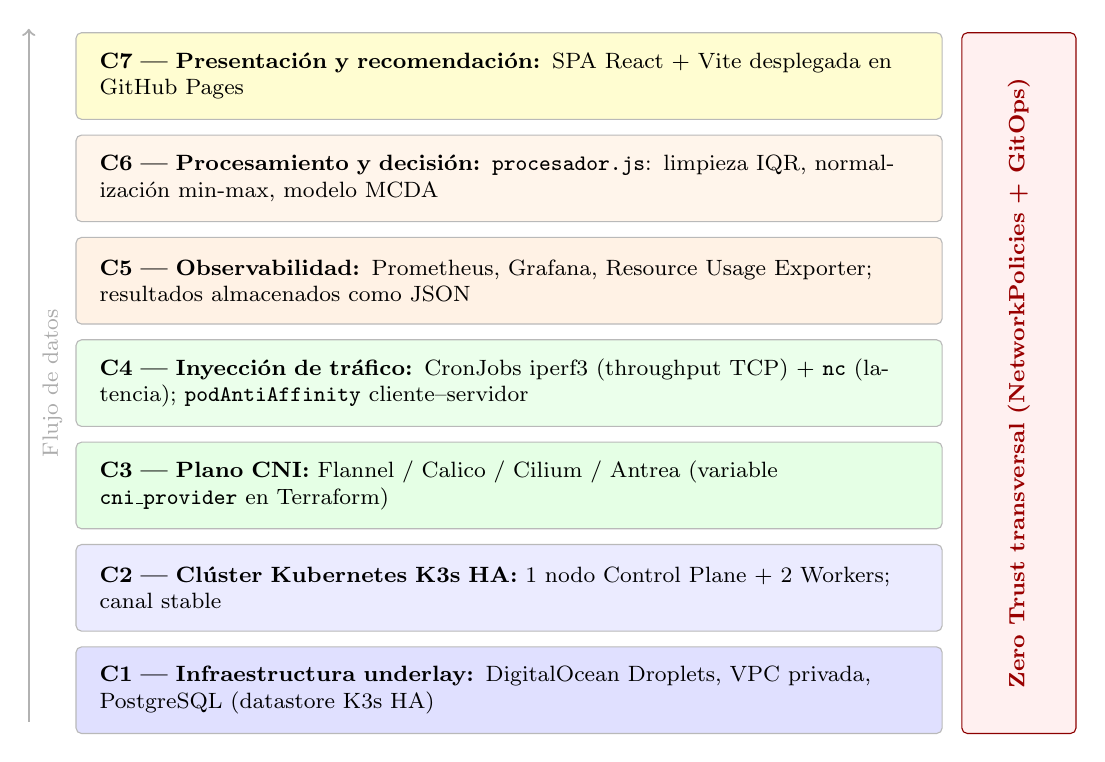
\begin{tikzpicture}[font=\footnotesize]
\tikzset{lay/.style={draw=gray!55, minimum width=11cm, minimum height=1.1cm,
    text width=10.4cm, align=left, inner sep=4pt, rounded corners=2pt}}

\node[lay, fill=blue!12] at (0,0.0)
    {\textbf{C1 --- Infraestructura underlay:} DigitalOcean Droplets, VPC privada, PostgreSQL (datastore K3s HA)};
% VERIFICAR: anclar versión exacta de K3s también aquí cuando se recupere de los logs
\node[lay, fill=blue!8] at (0,1.3)
    {\textbf{C2 --- Clúster Kubernetes K3s HA:} 1 nodo Control Plane + 2 Workers; canal stable};
\node[lay, fill=green!10] at (0,2.6)
    {\textbf{C3 --- Plano CNI:} Flannel / Calico / Cilium / Antrea (variable \texttt{cni\_provider} en Terraform)};
\node[lay, fill=green!8] at (0,3.9)
    {\textbf{C4 --- Inyección de tráfico:} CronJobs iperf3 (throughput TCP) + \texttt{nc} (latencia); \texttt{podAntiAffinity} cliente--servidor};
\node[lay, fill=orange!10] at (0,5.2)
    {\textbf{C5 --- Observabilidad:} Prometheus, Grafana, Resource Usage Exporter; resultados almacenados como JSON};
\node[lay, fill=orange!8] at (0,6.5)
    {\textbf{C6 --- Procesamiento y decisión:} \texttt{procesador.js}: limpieza IQR, normalización min-max, modelo MCDA};
\node[lay, fill=yellow!18] at (0,7.8)
    {\textbf{C7 --- Presentación y recomendación:} SPA React + Vite desplegada en GitHub Pages};

% Zero Trust transversal bar
\fill[red!6, draw=red!55!black, rounded corners=2pt] (5.75,-0.55) rectangle (7.20,8.35);
\node[rotate=90, font=\footnotesize\bfseries, text=red!60!black] at (6.475,3.90)
    {Zero Trust transversal (NetworkPolicies + GitOps)};

% Data flow arrow
\draw[->, thick, gray!60] (-6.10,-0.40) -- (-6.10,8.40);
\node[rotate=90, font=\footnotesize, text=gray!65] at (-5.80,3.90) {Flujo de datos};

\end{tikzpicture}
\caption{Arquitectura por capas del testbed experimental.}
\label{fig:arquitectura-capas}
\end{figure}
\shorthandon{>}

\section{Trazabilidad y Requisitos de Diseño}

El diseño no se planteó como una arquitectura aislada, sino como respuesta directa al problema formulado en el anteproyecto: las organizaciones adoptan Kubernetes como plataforma de orquestación, pero la calidad final del despliegue depende del plano de red, de la selección del CNI y del control de las comunicaciones internas del clúster \cite{ref29}. La Tabla~\ref{tab:trazabilidad-diseno} hace explícita la correspondencia entre cada necesidad, su objetivo asociado y la decisión de diseño que la atiende.

\begin{table}[htbp]
\centering
\scriptsize
\caption{Trazabilidad entre problema de investigación, objetivo y decisión de diseño.}
\label{tab:trazabilidad-diseno}
\begin{tabularx}{\textwidth}{|Y|Y|Y|}
\hline
\textbf{Necesidad identificada} & \textbf{Objetivo asociado} & \textbf{Respuesta de diseño} \\
\hline
Comparar CNIs sin depender de recomendaciones informales. & Evaluar cuantitativamente Calico, Cilium, Flannel y Antrea en escenarios controlados. & Testbed reproducible sobre Kubernetes, ejecución automatizada y consolidación de métricas por CNI. \\
\hline
Controlar el riesgo de comunicaciones internas abiertas. & Evaluar políticas de red seguras y automatizadas. & NetworkPolicies bajo enfoque Zero Trust, casos de denegación por defecto y segmentación por capas. \\
\hline
Convertir resultados técnicos heterogéneos en una decisión comprensible. & Definir criterios, umbrales y ponderaciones para comparación objetiva. & Modelo MCDA con criterios de rendimiento, eficiencia de recursos e impacto de seguridad. \\
\hline
Apoyar a una organización que necesita seleccionar y configurar un CNI. & Implementar un prototipo funcional de recomendación. & Prototipo web que consume datos procesados, aplica perfiles de decisión y explica la recomendación. \\
\hline
Evitar sobredimensionamiento de infraestructura. & Relacionar desempeño de red con consumo de CPU y memoria. & Captura de recursos del CNI mediante Prometheus y cálculo de eficiencia relativa por perfil. \\
\hline
\end{tabularx}
\end{table}

De este planteamiento se derivan cinco requisitos de diseño. La \textbf{reproducibilidad} se obtiene mediante infraestructura como código, despliegue declarativo y automatización de experimentos. El \textbf{aislamiento de variables} mantiene constante todo elemento distinto del CNI ---proveedor, tipo de instancia, versión de Kubernetes, topología y duración---. La \textbf{medición integral} evalúa el CNI por rendimiento de red, eficiencia de recursos e impacto de seguridad, y no solo por throughput. La \textbf{trazabilidad de la evidencia} exige que cada dato conserve su origen. La \textbf{compatibilidad con la operación real} se logra empleando objetos y patrones nativos de Kubernetes ---Deployments, CronJobs, ArgoCD--- cercanos a la práctica de los equipos de operaciones.

\section{Prototipo Recomendador}

El prototipo recomendador es la capa de interacción entre el modelo matemático y el usuario final. Su salida comprende tres niveles: la recomendación directa (qué CNI se sugiere), la justificación (qué métricas la explican) y la orientación de configuración (qué consideraciones debe atender el usuario al desplegar ese CNI), estructura que responde al objetivo específico 4 del anteproyecto \cite{ref29}. Se implementó como SPA con React~19, Vite~7 y Tailwind CSS~3; el \emph{build} de producción se despliega en GitHub Pages, y la actualización de datos encadena \texttt{procesador.js} ---que genera \texttt{cni-data.json}--- con la inyección de esos datos en el \emph{bundle}.

\section{Alcance y Límites del Diseño}

El diseño se limita a evaluar CNIs en un testbed controlado sobre Kubernetes y no pretende generalizar automáticamente los resultados a cualquier proveedor, versión o hardware. Emplea tráfico TCP controlado como señal principal y no asume que una mayor complejidad implique un mejor resultado. La solución se concibió para sostener una mejora continua: a medida que se incorporen nuevas corridas o versiones de CNIs, el pipeline puede recalcular los puntajes. En lugar de entregar una decisión congelada, ofrece un método para decidir con evidencia actualizable: técnicamente, reemplaza opiniones por datos medidos en condiciones reproducibles; económicamente, conocer el consumo de CPU de cada CNI por unidad de tráfico permite dimensionar la infraestructura sin márgenes precautorios excesivos \cite{ref29}.


\chapter{La Herramienta: Implementación y Despliegue} \label{cap:herramienta}

El diseño del capítulo anterior se materializa en una herramienta concreta, automatizada y reproducible: un \emph{testbed} de evaluación desplegado como infraestructura como código, un motor de decisión multicriterio y un prototipo recomendador que expone las recomendaciones a las organizaciones. Este es el producto central del trabajo de grado. La infraestructura está codificada en Terraform, la configuración en manifiestos YAML versionados en Git y las pruebas automatizadas en CronJobs de Kubernetes ---condición necesaria para que los resultados sean reproducibles y atribuibles al CNI. El manual de usuario y el manual de instalación se incluyen como anexos.


La infraestructura está codificada en Terraform, la configuración en manifiestos YAML versionados en Git y las pruebas automatizadas en CronJobs de Kubernetes ---condición necesaria para que los resultados sean reproducibles y atribuibles al CNI.

\section{Aprovisionamiento de Infraestructura con Terraform}

El aprovisionamiento de servidores y redes se realizó mediante Terraform (IaC). Al describir la infraestructura en archivos versionados, Terraform la recrea de manera idéntica en cada ejecución y elimina la posibilidad de que variaciones manuales introduzcan diferencias entre los entornos de cada CNI.

\subsection{Estructura del Código Terraform (K8s-bootstrap/00.bootstrap)}

\begin{table}[htbp]
\centering
\scriptsize
\renewcommand{\arraystretch}{1.25}
\setlength{\tabcolsep}{4pt}
\caption{Archivos Terraform del módulo de aprovisionamiento y su función específica.}
\label{tab:terraform-aprovisionamiento}
\begin{tabularx}{\textwidth}{|l|Y|}
\hline
\textbf{Archivo Terraform} & \textbf{Responsabilidad en la Infraestructura} \\
\hline
\texttt{main.tf} & Define los recursos principales: Droplets de DigitalOcean y red VPC privada. \\
\hline
\texttt{variables.tf} & Centraliza todos los parámetros configurables: número de nodos (\texttt{agent\_count = 2}), tamaño de instancias, región y proveedor CNI. \\
\hline
\texttt{ssh\_keys.tf} & Automatiza la gestión de llaves SSH para el acceso seguro entre nodos. \\
\hline
\texttt{firewall.tf} & Configura las reglas de firewall a nivel de nube: primera línea de seguridad perimetral. \\
\hline
\texttt{outputs.tf} & Genera automáticamente el archivo kubeconfig con las credenciales del clúster K3s. \\
\hline
\end{tabularx}
\end{table}

El proceso de aprovisionamiento tiene tres etapas: \texttt{terraform plan} (compara estado actual vs. código), \texttt{terraform apply} (crea Droplets, VPC y firewall) y \texttt{terraform output} (extrae IPs y kubeconfig). Terraform mantiene un archivo \texttt{terraform.tfstate} que permite destruir y recrear toda la infraestructura de manera controlada, garantizando la repetibilidad científica: cada CNI se evaluó en condiciones idénticas de arranque.

\section{Configuración del Clúster K3s en Alta Disponibilidad}

Una vez aprovisionados los servidores, se instaló y configuró K3s, una distribución liviana de Kubernetes, con topología de 1 nodo Master + 2 nodos Worker dedicados.

\subsection{Base de Datos Externa para el Plano de Control}

El plano de control se configuró con una base de datos PostgreSQL gestionada de DigitalOcean (también provisionada via Terraform) como datastore externo. Esto elimina la complejidad de mantener un clúster etcd y garantiza un plano de control sin punto único de fallo (SPOF).

\subsection{Instalación: clúster sin CNI para plugins externos y modo nativo para Flannel}

La implementación establece una distinción metodológica deliberada: Flannel se evalúa en su modo de despliegue más habitual ---integrado nativamente en K3s con \texttt{flannel-iface: eth1}---, mientras que Calico, Cilium y Antrea se instalan como plugins externos sobre un clúster sin CNI. La asimetría refleja las condiciones reales de uso: Flannel es el CNI predeterminado de K3s y la mayoría de equipos lo adopta sin configuración adicional, en tanto que los otros tres requieren instalación explícitamente y de forma declarativa. Evaluar cada CNI en su escenario de despliegue típico aumenta la validez ecológica del experimento; debe considerarse, no obstante, que Flannel se beneficia de la integración nativa de K3s ---gestión automática de CIDR y \emph{hooks} de kubelet--- que los plugins externos deben replicar por su cuenta.

Para los CNIs externos, la configuración crítica es el parámetro \texttt{--flannel-backend=none}, que desactiva completamente el CNI integrado de K3s y evita interferencias con el plugin bajo evaluación. Adicionalmente, se configura \texttt{--disable-network-policy} para que K3s no intente implementar NetworkPolicies por sí mismo.

La configuración resultante en \texttt{/etc/rancher/k3s/config.yaml} para CNIs externos incluye:
\begin{lstlisting}
flannel-backend: none
disable-network-policy: true
\end{lstlisting}

\begin{table}[htbp]
\centering
\scriptsize
\renewcommand{\arraystretch}{1.25}
\setlength{\tabcolsep}{4pt}
\caption{Instalación de CNIs: método y configuración clave en \texttt{user\_data/ks3\_server\_init.sh}.}
\label{tab:cni-instalacion}
\begin{tabularx}{\textwidth}{|l|p{3.2cm}|Y|}
\hline
\textbf{CNI} & \textbf{Método de instalación} & \textbf{Configuración clave} \\
\hline
Flannel & Nativo K3s & \texttt{flannel-iface: eth1} (interfaz VPC de DigitalOcean) \\
\hline
Calico & Tigera Operator v3.29.1 & \texttt{encapsulation: VXLAN}, CIDR \texttt{10.42.0.0/16}, \texttt{nodeAddressAutodetectionV4.interface: eth1} \\
\hline
Cilium & Helm 1.16.5 & \texttt{routingMode=tunnel}, \texttt{tunnelProtocol=vxlan}, \texttt{ipam.mode=kubernetes}, \texttt{devices=eth1}, \texttt{operator.replicas=1} \\
\hline
Antrea & Manifest v2.2.0 & \texttt{transportInterface: eth1}, \texttt{serviceCIDR: 10.43.0.0/16} \\
\hline
\end{tabularx}
\end{table}

El protocolo de rotación de CNIs se implementó mediante el reemplazo completo de la infraestructura entre ciclos. Para cambiar de un CNI al siguiente, se modificó la variable \texttt{cni\_provider} en \texttt{terraform.tfvars} y se ejecutó \texttt{terraform destroy} seguido de \texttt{terraform apply}: el primero eliminó todos los recursos de DigitalOcean (Droplets, VPC y base de datos PostgreSQL), y el segundo los recreó desde cero con el nuevo CNI preconfigurado en el script de inicialización de K3s. Este enfoque garantiza que cada ciclo de prueba parte de nodos completamente limpios, sin residuos de configuración del CNI anterior que pudieran contaminar las métricas.

\section{Orquestación y Entrega Continua: GitOps con ArgoCD}

Con el clúster K3s funcionando y sin CNI, el siguiente componente instalado fue ArgoCD. ArgoCD implementa el paradigma GitOps: el repositorio Git es la única fuente de verdad sobre el estado del clúster. Todo lo que debe existir en el clúster está definido en archivos YAML dentro del repositorio \texttt{K8s-Tesis-Apps}. Esta centralización en Git facilita la auditoría del experimento: cualquier cambio en la configuración queda registrado con autor, fecha y motivo, haciendo el proceso de prueba completamente trazable.

\subsection{El Patrón App of Apps}

La implementación de ArgoCD utiliza el patrón App of Apps: existe UNA sola aplicación raíz (ubicada en \texttt{K8s-bootstrap/30.apps-of-apps-install}) que ArgoCD conoce directamente, y esa aplicación raíz contiene las definiciones de todas las demás aplicaciones (CNIs, stack de métricas, benchmarks, políticas de red).

\subsection{Configuración de selfHeal y prune}

\textbf{\emph{selfHeal: true}} --- Ante la modificación manual de un recurso del clúster ---por ejemplo, la eliminación de una NetworkPolicy---, ArgoCD detecta la diferencia con el repositorio Git y restaura el estado original, lo que resultó crítico para la integridad del experimento.

\textbf{\emph{prune: true}} --- Al eliminar un archivo YAML del repositorio Git, ArgoCD elimina también el recurso correspondiente del clúster, lo que evita la acumulación de recursos huérfanos.

\begin{lstlisting}
# Definicion de la Application raiz en ArgoCD (App of Apps)
apiVersion: argoproj.io/v1alpha1
kind: Application
metadata:
  name: apps-of-apps
  namespace: argocd
spec:
  source:
    repoURL: https://github.com/DuwanSierra/K8s-Tesis-Apps
    targetRevision: main
    path: apps/
  syncPolicy:
    automated:
      selfHeal: true   # Restaura cambios manuales automaticamente
      prune: true      # Elimina recursos borrados del repo
\end{lstlisting}

\subsection{Overlays de Kustomize para los CNIs}

Cada CNI tiene una configuración ligeramente diferente. Para gestionarlas sin duplicar código, se utilizó Kustomize con el patrón base/overlay: existe una configuración base con los parámetros comunes, y sobre esa base se aplican overlays específicas para cada CNI.

Las apps gestionadas por ArgoCD incluyen: \texttt{cni-test-iperf} (benchmarks de throughput y latencia), \texttt{cni-resource-exporter} (exportación de recursos desde Prometheus), \texttt{cni-np-test} (pruebas de Network Policies, creada solo cuando \texttt{cni\_provider != "flannel"} y el caso de uso está definido), y \texttt{metrics} (Prometheus + Grafana).

\section{Implementación del Stack de Observabilidad}

El stack de observabilidad se implementó mediante el \texttt{kube-prometheus-stack} (Helm chart) que instala Prometheus, Grafana y exportadores preconfigurados para Kubernetes.

\subsection{Prometheus: El Recolector de Métricas}

Prometheus opera con un modelo pull: visita periódicamente los endpoints de métricas (cada 15 segundos en la configuración del proyecto). Para que Prometheus sepa qué métricas recolectar de los agentes CNI, se implementaron \texttt{ServiceMonitors} (CRD), apuntando específicamente al endpoint de métricas de cada agente. Un intervalo de 15 segundos proporciona suficiente granularidad para detectar picos de consumo durante las ráfagas de tráfico iperf3, sin generar una carga de scraping que interfiera con las métricas bajo observación.

Las métricas clave recolectadas del agente CNI incluyen:
\begin{itemize}
\item \path|container_cpu_usage_seconds_total| (filtrado por pod del agente): costo computacional del CNI (criterio C2 del marco MCDA).
\item \path|container_memory_rss| (filtrado por pod del agente): memoria física real del proceso del agente CNI.
\item \path|node_network_transmit_bytes_total| / \path|node_network_receive_bytes_total|: bytes totales de red por nodo.
\item \path|kube_pod_info| + \path|kube_pod_status_phase|: estado del agente CNI para detectar reinicios durante las pruebas.
\end{itemize}

\subsection{Grafana: Los Dashboards de Red}

Grafana centraliza la lectura operativa de las series de Prometheus. Sus paneles agrupan throughput, latencia, consumo del agente CNI y score MCDA. Esta correlación vincula ráfagas iperf3 con CPU, RSS y el ranking calculado por \texttt{procesador.js}.

\subsection{Resource Usage Exporter: Extracción Automatizada de Datos}

El \texttt{cni-resource-usage-exporter} corre como CronJob en \path|K8s-Tesis-Apps/grafana-exporter|. ArgoCD sincroniza el recurso mediante la app \texttt{cni-resource-exporter}. El CronJob:
\begin{itemize}
\item Ejecuta la extracción en los minutos 25 y 55 de cada hora, tras cada ventana de benchmarks.
\item Consulta directamente la API HTTP de Prometheus (\texttt{/api/v1/query\_range}) --- no interactúa con Grafana.
\item Recolecta CPU\% por nodo, RAM\% por nodo, RAM usada, CPU cores y RAM del agente CNI.
\item Genera \texttt{raw/}, \texttt{csv/}, \texttt{images/} y \texttt{cni\_resource\_summary.json} por corrida.
\item Persiste cada salida con timestamp en \path|K8S-CNI-Results/results/cni-benchmarks/{cni}/resource_usage_nodes/|.
\end{itemize}

\section{Implementación del Banco de Pruebas de QoS}

\subsection{Escenario de Rendimiento con iperf3}

El banco de throughput se define en \texttt{K8s-Tesis-Apps/cni\_test\_iperf}:

\textbf{El iperf3-server (Deployment):} Un Deployment ejecuta una réplica de iperf3 en modo servidor. Un Service ClusterIP expone un nombre DNS estable para el cliente.

\textbf{El iperf3-client (CronJob):} La programación \texttt{0,30 * * * *} activa el cliente en los minutos 0 y 30. \texttt{concurrencyPolicy: Forbid} bloquea corridas simultáneas. Cada activación crea un Pod y genera tráfico TCP durante 300 segundos. La salida conserva formato JSON con \texttt{iperf3 -t 300 -i 10 -J}. La retención máxima queda en 5 corridas (\texttt{RETENTION\_MAX\_RUNS="5"}).

La anti-afinidad del cliente frente al servidor se implementó como \texttt{preferredDuringSchedulingIgnoredDuringExecution} (suave, weight 100), forzando tráfico inter-nodo en la práctica. Esta ubicación garantiza que todo el tráfico de benchmark atraviese el mecanismo de encapsulación del CNI entre nodos, que es exactamente lo que se quiere medir.

\begin{lstlisting}
# iperf-client-cronjob.yaml -- fragmento relevante
schedule: '0,30 * * * *'   # Minutos 0 y 30
concurrencyPolicy: Forbid
affinity:
  podAntiAffinity:
    preferredDuringSchedulingIgnoredDuringExecution:
    - weight: 100
      podAffinityTerm:
        labelSelector:
          matchLabels:
            app: iperf-server
        topologyKey: kubernetes.io/hostname
# iperf3 -c iperf-server-svc -t 300 -i 10 -J
\end{lstlisting}

\subsection{Cliente de Latencia Personalizado}

El CronJob \texttt{latency-client-cronjob.yaml} ejecuta la prueba de latencia. Su programación corre en los minutos 10 y 40 de cada hora. Esa separación evita solapamiento con el inicio del throughput.

El cliente registra TCP Connect con \texttt{nc -z -w 2} y timestamp en ms. Cada corrida toma 30 muestras y calcula min/avg/max/mdev. El JSON normalizado conserva campos de latencia, muestras intentadas y muestras exitosas.

\begin{table}[htbp]
\centering
\scriptsize
\renewcommand{\arraystretch}{1.25}
\setlength{\tabcolsep}{4pt}
\caption{Métricas de QoS capturadas por el banco de pruebas y su relevancia telemática.}
\label{tab:metricas-qos-implementacion}
\begin{tabularx}{\textwidth}{|p{4cm}|p{2.4cm}|Y|}
\hline
\textbf{Métrica Capturada} & \textbf{Unidad} & \textbf{Relevancia para QoS Telemático} \\
\hline
Throughput TCP sostenido & Gbps / Mbps & Capacidad efectiva de la red. \\
\hline
Latencia mínima TCP connect & ms & Overhead mínimo del CNI sin congestión. \\
\hline
Latencia promedio TCP connect & ms & Comportamiento típico de solicitudes. \\
\hline
Latencia máxima / Jitter & ms & Peor caso y variabilidad. Crítico para tiempo real. \\
\hline
Retransmisiones TCP & count / sesión & Indicador de problemas en encapsulamiento o congestión. \\
\hline
CPU del agente CNI & millicores (m) & Impacto directo en costo de infraestructura cloud. \\
\hline
RAM del agente CNI (RSS) & MiB & Huella de memoria del agente CNI por nodo. \\
\hline
\end{tabularx}
\end{table}

\section{Procesamiento Estadístico y Aplicación del Modelo MCDA}

\subsection{Limpieza con el Rango Intercuartílico (IQR)}

\texttt{docs/procesador.js} transforma datos crudos en datos consolidados. El script descubre los CNIs disponibles bajo \texttt{results/cni-benchmarks}. Luego extrae métricas desde JSON y CSV. Finalmente aplica IQR:

\begin{lstlisting}
// procesador.js -- Funcion de limpieza estadistica IQR
function calcularEstadisticasLimpias(valores) {
  const sorted = [...valores].sort((a, b) => a - b);
  const q1 = sorted[Math.floor(sorted.length * 0.25)];
  const q3 = sorted[Math.floor(sorted.length * 0.75)];
  const iqr = q3 - q1;
  const lowerBound = q1 - 1.5 * iqr;
  const upperBound = q3 + 1.5 * iqr;
  const valoresLimpios = valores.filter(
    v => v >= lowerBound && v <= upperBound);
  const promedio = valoresLimpios.reduce(
    (sum, v) => sum + v, 0) / valoresLimpios.length;
  return { promedio,
    outliersPorcentaje: ((valores.length - valoresLimpios.length)
      / valores.length * 100).toFixed(1)
  };
}
\end{lstlisting}

El pipeline descarta valores atípicos antes de calcular promedios. Dado que un evento cloud anómalo puede sesgar una corrida, el filtro estabiliza el puntaje MCDA del CNI.

\subsection{Normalización y Cálculo del Score MCDA}

Después de la limpieza, el pipeline aplica la normalización min-max re-escalada a $[1,\,5]$ descrita en el Marco Teórico. En métricas positivas como throughput, la normalización es directa ($V_i = 5$ al máximo). En métricas negativas como latencia o CPU, el cociente se invierte, de modo que el valor más bajo recibe $V_i = 5$ y el más alto $V_i = 1$. La escala uniforme permite comparar Gbps, milisegundos y millicores sin sesgo por magnitud numérica.

\begin{lstlisting}
// recommendationModel.js -- Calculo del overhead de seguridad
function getNetworkPolicyOverhead(data) {
  if (!data?.network_policy) return null;
  const caseValues = Object.values(data.network_policy).flatMap(
    (policyCase) => [
      Number(policyCase?.overhead_latencia_pct),
      Number(policyCase?.overhead_throughput_pct),
  ]);
  const validValues = caseValues.filter((v) => Number.isFinite(v));
  if (!validValues.length) return null;
  return average(validValues);
}
// El score de seguridad se invierte (menor overhead = 5.0).
// Si meta.supportsNetworkPolicy === false (ej. Flannel), el score es 1.
\end{lstlisting}

El pipeline calcula el puntaje de la dimensión de seguridad evaluando el impacto (\emph{overhead}) promedio en latencia y throughput al activar los casos de prueba de \texttt{network\_policy}. Entre menor sea la degradación del rendimiento al aislar los Pods, mayor será la calificación normalizada del CNI. Aquellos plugins que por diseño no implementan Network Policies en su plano de datos reciben por defecto la calificación mínima de $1.00$ en esta dimensión, penalizando su uso en entornos que requieran aislamiento lógico.

\section{Prototipo Recomendador: Aplicación Web SPA}

\subsection{Tecnologías de Implementación}

La SPA fue implementada con React~19 (gestión de estado por componentes), Vite~7 (bundler; build de producción vía \texttt{build:pages} con \texttt{--outDir ../docs/recommender}) y Tailwind CSS~3 (estilos utilitarios directamente en JSX, sin CSS personalizado).

\texttt{npm run sync:data} ejecuta \texttt{procesador.js} y genera \texttt{cni-data.json}. Después, \texttt{export-spa-data.cjs} inyecta los datos en el bundle. \texttt{recommendationModel.js} concentra la lógica de recomendación.

\subsection{Flujo de la Aplicación}

\begin{enumerate}
\item \textbf{Selección de Perfil:} La pantalla principal muestra tres tarjetas: Fintech/Seguridad, Streaming/Rendimiento e IoT/Recursos.
\item \textbf{Visualización de Resultados:} La aplicación carga \texttt{cni-data.json} y calcula el ranking MCDA para el perfil seleccionado. El CNI con mayor puntaje queda marcado como recomendación.
\item \textbf{Justificación Técnica:} La interfaz expone las métricas brutas promedio de cada CNI en gráficas comparativas.
\end{enumerate}

\section{Implementación de Network Policies y Seguridad Zero Trust}

\subsection{Políticas Default Deny}

Default Deny operacionaliza el modelo Zero Trust. La política bloquea todo el tráfico inicial y habilita solo comunicaciones necesarias. Con esta regla, toda comunicación no autorizada falla sin intervención del operador.

El siguiente manifiesto aplica la política a todos los Pods del namespace \texttt{production}:

\begin{lstlisting}
# default-deny-all.yaml
apiVersion: networking.k8s.io/v1
kind: NetworkPolicy
metadata:
  name: default-deny-all
  namespace: production
spec:
  podSelector: {}     # aplica a TODOS los Pods del namespace
  policyTypes:
  - Ingress           # Bloquea todo el trafico entrante
  - Egress            # Bloquea todo el trafico saliente
\end{lstlisting}

\subsection{Micro-segmentación por Capas de Aplicación}

Sobre Default Deny, las políticas específicas acotan el tráfico permitido. Las reglas \texttt{frontend $\rightarrow$ backend $\rightarrow$ database} usan label selectors.

En Cilium, una \texttt{CiliumNetworkPolicy} de capa 7 admite solo métodos \texttt{GET} y \texttt{HEAD} desde frontend hacia backend. En Antrea, una \texttt{ClusterNetworkPolicy} en el Tier \texttt{securityops} prioriza sobre cualquier \texttt{NetworkPolicy} de namespace.

Esta estratificación evalúa seguridad granular en condiciones reales. También cuantifica si esa granularidad introduce overhead detectable, uno de los criterios del modelo MCDA.

\subsection{Validación Automatizada de Políticas}

Se implementó un pipeline de validación que emplea \texttt{nc} (netcat) dentro de Pods de prueba para verificar la conectividad. Para cada par de Pods, el pipeline define una expectativa ---la conexión debe permitirse o debe bloquearse--- y reporta un error cuando el comportamiento observado no coincide con ella.

\begin{table}[htbp]
\centering
\scriptsize
\renewcommand{\arraystretch}{1.25}
\setlength{\tabcolsep}{4pt}
\caption{Casos de prueba del pipeline de validación de Network Policies.}
\label{tab:validacion-network-policies}
\begin{tabularx}{\textwidth}{|p{5cm}|Y|}
\hline
\textbf{Prueba de Validación} & \textbf{Resultado Esperado y Justificación} \\
\hline
frontend $\rightarrow$ backend (puerto 8080) & PERMITIDO --- Comunicación necesaria para el funcionamiento de la aplicación. \\
\hline
frontend $\rightarrow$ database (puerto 5432) & BLOQUEADO --- El frontend no debe acceder directamente a la base de datos. \\
\hline
backend $\rightarrow$ database (puerto 5432) & PERMITIDO --- El backend necesita leer y escribir datos. \\
\hline
database $\rightarrow$ cualquier Pod & BLOQUEADO --- La base de datos nunca debe iniciar conexiones salientes. \\
\hline
Pod externo $\rightarrow$ namespace production & BLOQUEADO --- Sin una regla explícita, ningún Pod externo puede entrar. \\
\hline
\end{tabularx}
\end{table}

\section{Estructura de Repositorios y Entregables Técnicos}

La Tabla~\ref{tab:repositorios-entregables} resume la organización del proyecto en cuatro repositorios Git.

\begin{table}[htbp]
\centering
\scriptsize
\renewcommand{\arraystretch}{1.25}
\setlength{\tabcolsep}{4pt}
\caption{Estructura de los cuatro repositorios del proyecto y su relación con los objetivos específicos.}
\label{tab:repositorios-entregables}
\begin{tabularx}{\textwidth}{|p{3cm}|Y|p{5.2cm}|}
\hline
\textbf{Repositorio} & \textbf{Contenido Principal} & \textbf{Relación con los Objetivos} \\
\hline
\texttt{HA-K3s-Terraform-DO} & Módulo Terraform reutilizable que provisiona Droplets, VPC, Load Balancer y base de datos PostgreSQL en DigitalOcean. & OE1: Módulo base de infraestructura cloud invocado por \texttt{K8s-bootstrap}. \\
\hline
\texttt{K8s-bootstrap} & Código Terraform (\texttt{00.bootstrap}), scripts de instalación K3s HA (\texttt{10.k3s-ha-do}), manifiestos de ArgoCD (\texttt{20.argo-cd-install}) y App of Apps (\texttt{30.apps-of-apps-install}). & OE1: Orquesta el aprovisionamiento completo del testbed. \\
\hline
\texttt{K8s-Tesis-Apps} & Overlays Kustomize para los 4 CNIs, stack de observabilidad (\texttt{apps/metrics}), benchmarks iperf3 (\texttt{cni\_test\_iperf}), cliente de latencia, Network Policies y Grafana Exporter. & OE1, OE2 y OE3: Implementa las pruebas, la seguridad y el sistema de recolección. \\
\hline
\texttt{K8S-CNI-Results} & Archivos JSON/CSV con resultados por corrida, \texttt{procesador.js} (modelo MCDA) y la SPA recomendadora (\texttt{cni-recommender-spa}). & OE3 y OE4: Implementa el modelo de comparación objetiva y el prototipo. \\
\hline
\end{tabularx}
\end{table}

La arquitectura mantiene un flujo unidireccional: \texttt{HA-K3s-Terraform-DO} provee el módulo cloud; \texttt{K8s-bootstrap} orquesta la infraestructura; \texttt{K8s-Tesis-Apps} despliega las aplicaciones y genera métricas; \texttt{K8S-CNI-Results} almacena, procesa y visualiza resultados.

\section{Desafíos de Implementación y Soluciones Adoptadas}

\begin{table}[htbp]
\centering
\scriptsize
\renewcommand{\arraystretch}{1.25}
\setlength{\tabcolsep}{4pt}
\caption{Desafíos técnicos encontrados durante la implementación y soluciones adoptadas.}
\label{tab:desafios-implementacion}
\begin{tabularx}{\textwidth}{|Y|Y|}
\hline
\textbf{Desafío Encontrado} & \textbf{Solución Técnica Implementada} \\
\hline
MTU mismatch al instalar Cilium: Pods no podían comunicarse, paquetes se fragmentaban silenciosamente en la VPC. Flannel y Calico detectan automáticamente la MTU de la interfaz subyacente en sus versiones actuales; Cilium requirió configuración explícita porque su dataplane eBPF no hereda el valor de MTU del sistema operativo sin intervención. & Se calculó la MTU efectiva: 1500 (VPC) $-$ 50 (overhead VXLAN) $=$ 1450. Se configuró el parámetro \texttt{mtu: 1450} en el overlay de Kustomize de Cilium. \\
\hline
ArgoCD en estado OutOfSync al instalar el stack de métricas (Prometheus + Grafana): los CRDs del \texttt{kube-prometheus-stack} se aplicaban en el mismo ciclo de sync que los recursos que los consumían, provocando fallo en el despliegue porque el API server aún no conocía los tipos personalizados. & Se separó la instalación en dos Applications independientes usando sync waves: \texttt{kube-prometheus-stack-crds} (wave~$-1$) despliega el mismo chart con todos los componentes deshabilitados ---solo crea los CRDs--- usando \texttt{ServerSideApply=true}; \texttt{kube-prometheus-stack} (wave~$0$) despliega el stack completo con \texttt{skipCrds:~true} y \texttt{SkipDryRunOnMissingResource=true}, garantizando que los CRDs existen antes de crear los recursos dependientes. \\
\hline
Outliers frecuentes en pruebas de madrugada: DigitalOcean mostraba throttling de CPU en horas de alta demanda del datacenter. & Se configuró una ventana de pruebas exclusiva para horario laboral. El algoritmo IQR filtra automáticamente estos outliers. \\
\hline
\texttt{procesador.js} necesitaba evaluar la seguridad de forma cuantitativa e integrada en el MCDA, pero Flannel no reportaba overhead al no soportar políticas. & Se parametrizó el score de seguridad basándose en el overhead de latencia de las políticas. Para los CNIs que no soportan políticas (Flannel), el modelo asigna directamente el puntaje mínimo de $1.0$ en la dimensión de seguridad. \\
\hline
\end{tabularx}
\end{table}

\section{Flujo completo de ejecución}


% --- Parte IV: Validación y cierre ---
\chapter{Resultados y Pruebas} \label{sec:Resultados}

En cada ciclo de prueba se modificó únicamente el CNI bajo evaluación; hardware, sistema operativo, versión de Kubernetes, tamaño de paquetes, duración y condiciones de red permanecieron constantes, lo que hace posible atribuir las diferencias observadas al plugin y no al entorno.

\section{Metodología General de Pruebas}

\subsection{Control de Condiciones: el Escenario de Referencia}

Se definió un escenario de referencia con los siguientes parámetros fijos para todos los CNIs:

\begin{table}[htbp]
\centering
\scriptsize
\caption{Parámetros del escenario de referencia para todas las pruebas.}
\label{tab:baseline-pruebas}
\begin{tabularx}{\textwidth}{|Y|Y|}
\hline
\textbf{Parámetro Controlado} & \textbf{Valor Fijo para Todo el Experimento} \\
\hline
Tipo de instancia cloud & DigitalOcean Droplet --- Ubuntu 22.04 LTS, 2 vCPU, 4 GB RAM para nodos Worker \\
\hline
Versión de Kubernetes & K3s canal stable --- la misma versión en todos los ciclos de prueba \\
\hline
Región del datacenter & nyc3 (Nueva York) --- mismo datacenter para todos los nodos en todas las pruebas \\
\hline
Red entre nodos & VPC privada DigitalOcean --- MTU 1500 bytes, sin tráfico externo \\
\hline
Duración de cada prueba iperf3 & 300 segundos (5 minutos) por corrida \\
\hline
Número de corridas por CNI & 5 corridas independientes --- permite calcular promedios y detectar variabilidad \\
\hline
Protocolo de red bajo prueba & TCP --- el protocolo dominante en aplicaciones empresariales reales \\
\hline
Herramienta de throughput & iperf3 con salida JSON (\texttt{-J}), un solo stream TCP (\texttt{-P 1}) \\
\hline
Herramienta de latencia & Script Bash con \texttt{nc -z -w 2} --- 30 muestras por corrida \\
\hline
\end{tabularx}
\end{table}

\subsection{Automatización: de la Prueba Manual a la Prueba Orquestada}

Todas las pruebas se orquestaron mediante CronJobs de Kubernetes. La secuencia de ejecución automática en cada ciclo fue:
\begin{enumerate}
\item CronJob del cliente iperf3 se activa (minutos 0 y 30). Kubernetes crea el Pod cliente en un nodo diferente al servidor (podAntiAffinity suave, weight 100).
\item Pod cliente ejecuta iperf3 durante 300 segundos y guarda el resultado JSON.
\item CronJob del cliente de latencia ejecuta 30 mediciones de TCP connect (minutos 10 y 40) y guarda su resultado JSON.
\item Al finalizar ambas pruebas, el Resource Usage Exporter (minutos 25 y 55) consulta Prometheus para extraer el consumo de CPU y RAM del agente CNI.
\item \texttt{procesador.js} actualiza \texttt{cni-data.json} con los nuevos datos procesados.
\end{enumerate}

La orquestación automática elimina la variabilidad humana de la ejecución: cada corrida sigue exactamente la misma secuencia con los mismos intervalos, de modo que las diferencias observadas entre CNIs se deben al plugin y no al operador.

La elección de cinco corridas por CNI responde a un equilibrio entre rigor estadístico y viabilidad operativa. Una sola corrida permitiría que un dato atípico o evento anómalo dominara el resultado, mientras que un número muy elevado extendería el tiempo de prueba sin un beneficio proporcional. Con cinco corridas distribuidas en el tiempo, el algoritmo IQR puede identificar y descartar una corrida anómala, y el promedio de las restantes resulta estadísticamente representativo; este criterio es habitual en la investigación de redes sobre entornos cloud \cite{ref7,ref8}.

\section{Pruebas de Rendimiento de Red --- Objetivo Específico 1}

\subsection{Protocolo de Prueba de Throughput con iperf3}

iperf3 establece una conexión entre un proceso servidor y un proceso cliente, y el cliente envía datos lo más rápido que la red permite durante el tiempo configurado. Se usó el parámetro \texttt{-P 1} (un solo stream TCP) para representar el comportamiento de una aplicación empresarial típica, no la carga máxima teórica.

\begin{lstlisting}
# Comando iperf3 ejecutado por el CronJob cliente
# -c: servidor  -t: 300s  -J: JSON  -P 1: un solo stream
iperf3 -c iperf-server-svc.cni-benchmark.svc.cluster.local \
  -t 300 -J -P 1 \
  > /results/throughput-$(date +%Y%m%d_%H%M%S)-${CNI_NAME}.json
\end{lstlisting}

\subsection{Resultados de Throughput TCP por CNI}

Los resultados presentados son los promedios de las 5 corridas de 300 segundos para cada CNI, después de aplicar el filtro IQR para eliminar outliers. La Tabla~\ref{tab:throughput-resultados} registra tres dimensiones de calidad del canal: cuántos datos por segundo puede transportar (throughput), cuántos paquetes tuvieron que reenviarse por error (retransmisiones) y qué tan predecible es el canal entre corridas (variabilidad).

\begin{table}[htbp]
\centering
\scriptsize
\caption{Resultados de rendimiento TCP por CNI (promedio de 5 corridas de 300 segundos, outliers IQR eliminados).}
\label{tab:throughput-resultados}
\begin{tabularx}{\textwidth}{|Y|c|c|c|c|}
\hline
\textbf{Métrica} & \textbf{Flannel (VXLAN)} & \textbf{Calico (VXLAN)} & \textbf{Cilium (eBPF)} & \textbf{Antrea (OVS)} \\
\hline
Throughput promedio --- Mbps \newline\textit{($\uparrow$ mayor es mejor: más datos por segundo)} & 1452.97 & \textbf{1804.40} & 843.56 & 1588.45 \\
\hline
Retransmisiones TCP --- paquetes/sesión \newline\textit{($\downarrow$ menor es mejor: menos retransmisiones en el canal)} & \textbf{11774} & 68993 & 15142 & 42229 \\
\hline
Outliers descartados (Throughput) & 0 de 5 (0\%) & 0 de 5 (0\%) & 1 de 5 (20\%) & 0 de 5 (0\%) \\
\hline
Outliers descartados (Retransmisiones) & 0 de 5 (0\%) & 1 de 5 (20\%) & 0 de 5 (0\%) & 0 de 5 (0\%) \\
\hline
\end{tabularx}
\end{table}

A diferencia de los entornos locales de alto rendimiento, la red en nube VPC privada de DigitalOcean limita el ancho de banda efectivo, registrándose valores máximos de throughput de 1804.40 Mbps en Calico, seguido de Antrea con 1588.45 Mbps y Flannel con 1452.97 Mbps. Cilium presenta el valor más bajo con 843.56 Mbps. Las diferencias en retransmisiones TCP son críticas: Flannel destaca con la menor cantidad de retransmisiones (11774), seguido por Cilium (15142) y Antrea (42229), mientras que Calico registra la tasa de fallas más alta con 68993 retransmisiones. Esto indica que a pesar de que Calico lidera el throughput bruto, genera un mayor estrés de reenvío de paquetes debido a la saturación del datapath.

\subsection{Protocolo de Prueba de Latencia TCP}

La latencia reportada en este experimento no mide el tiempo de tránsito físico puro de la red (latencia de enlace L3/L4 intra-VPC, habitualmente inferior a 1 ms), sino el tiempo total de establecimiento de conexión TCP a nivel de aplicación. El cliente ejecuta un \emph{script} Bash iterando \texttt{nc -z -w 2} hacia el servicio \texttt{iperf3-server}, lo que captura no solo el \emph{handshake} de tres vías, sino el overhead del \emph{spawn} del proceso en el sistema operativo y la resolución DNS interna de Kubernetes en cada ciclo. Esta métrica de latencia final (12-35 ms) resulta útil para comparar el estrés relativo que cada CNI impone al stack de red bajo este tipo de rutinas de microservicios, pero los valores absolutos no deben interpretarse como la latencia base de la red virtual de DigitalOcean.

\subsection{Resultados de Latencia TCP por CNI}

En todas las filas de la Tabla~\ref{tab:latencia-resultados}, \textbf{un valor menor es mejor ($\downarrow$)}: menos milisegundos significa que el CNI establece conexiones más rápido. La latencia máxima refleja el comportamiento bajo condiciones adversas de carga de red, mientras que el Jitter (MDEV) mide la predictibilidad del enlace.

\begin{table}[htbp]
\centering
\scriptsize
\caption{Resultados de latencia TCP por CNI (30 muestras $\times$ 5 corridas, outliers IQR eliminados). Todas las métricas: $\downarrow$ menor es mejor.}
\label{tab:latencia-resultados}
\begin{tabularx}{\textwidth}{|Y|c|c|c|c|}
\hline
\textbf{Métrica de Latencia ($\downarrow$ menor=mejor)} & \textbf{Flannel (VXLAN)} & \textbf{Calico (VXLAN)} & \textbf{Cilium (eBPF)} & \textbf{Antrea (OVS)} \\
\hline
Latencia promedio --- ms \newline\textit{(comportamiento típico)} & 21.53 & \textbf{12.54} & 18.73 & 35.09 \\
\hline
Latencia máxima --- ms \newline\textit{(peor caso observado)} & 50.80 & \textbf{44.20} & 47.00 & 83.50 \\
\hline
Jitter (MDEV) --- ms \newline\textit{(variabilidad de la latencia)} & 7.76 & \textbf{7.31} & 8.47 & 17.25 \\
\hline
Outliers descartados (Latencia Max) & 0 de 5 (0\%) & 0 de 5 (0\%) & 0 de 5 (0\%) & 1 de 5 (20\%) \\
\hline
\end{tabularx}
\end{table}

Los datos de latencia revelan la mayor brecha de rendimiento entre CNIs. Calico logra la menor latencia promedio (12.54 ms) y el menor jitter (7.31 ms). Cilium se sitúa en segundo lugar con una latencia promedio de 18.73 ms, seguido por Flannel con 21.53 ms. Antrea registra el desempeño más bajo, alcanzando una latencia promedio de 35.09 ms y un jitter elevado de 17.25 ms (más del doble que Calico). Esto indica que para entornos donde el tiempo de establecimiento de conexión TCP es un factor de éxito (como APIs web interactivas), Calico ofrece la respuesta más rápida y estable.

\section{Pruebas de Seguridad con Network Policies --- Objetivo Específico 2}

\subsection{Matriz de Pruebas de Network Policies}

Se diseñó una matriz de pruebas que cubre los escenarios críticos de seguridad en un clúster Kubernetes. La herramienta de verificación principal fue \texttt{kubectl exec} combinada con \texttt{nc} (netcat) dentro de Pods de prueba.

\begin{table}[htbp]
\centering
\scriptsize
\caption{Matriz completa de pruebas de seguridad con Network Policies.}
\label{tab:matriz-seguridad}
\begin{tabularx}{\textwidth}{|Y|Y|}
\hline
\textbf{Caso de Prueba} & \textbf{Descripción, Herramienta y Criterio de Éxito} \\
\hline
TC-SEC-01: Default Deny Ingress & Ningún Pod externo puede enviar tráfico al namespace sin regla explícita. Verificación: \texttt{nc -zv <pod-ip> 8080}. ÉXITO: timeout en menos de 5 s. \\
\hline
TC-SEC-02: Default Deny Egress & Los Pods en producción no pueden iniciar conexiones salientes no autorizadas. Verificación: \texttt{curl --max-time 3}. ÉXITO: timeout. \\
\hline
TC-SEC-03: Frontend$\rightarrow$Backend permitido & Pod con etiqueta \texttt{tier=frontend} puede conectarse al backend en puerto 8080. ÉXITO: Connection succeeded. \\
\hline
TC-SEC-04: Bloqueo Frontend$\rightarrow$Database & Pod frontend NO puede conectarse a la base de datos directamente. ÉXITO: Connection refused o timeout. \\
\hline
TC-SEC-05: Backend$\rightarrow$Database permitido & Pod backend SÍ puede conectarse a la base de datos en puerto 5432. ÉXITO: Connection succeeded. \\
\hline
TC-SEC-06: Database NO inicia conexiones & La base de datos nunca inicia conexiones salientes. ÉXITO: Bloqueo por política de Egress. \\
\hline
TC-SEC-07: Bloqueo entre namespaces & Un Pod de namespace staging no puede comunicarse con Pods de production. ÉXITO: Bloqueo confirmado. \\
\hline
TC-SEC-08: GitOps Auto-restauración & Si una política se elimina manualmente, ArgoCD la restaura en menos de 3 minutos. ÉXITO: Política restaurada automáticamente. \\
\hline
\end{tabularx}
\end{table}

\subsection{Resultados de las Pruebas de Seguridad por CNI}

\begin{table}[htbp]
\centering
\scriptsize
\caption{Resultados de pruebas de seguridad por CNI.}
\label{tab:resultados-seguridad}
\begin{tabularx}{\textwidth}{|Y|Y|Y|Y|Y|}
\hline
\textbf{Caso de Prueba} & \textbf{Flannel} & \textbf{Calico} & \textbf{Cilium} & \textbf{Antrea} \\
\hline
TC-SEC-01: Default Deny Ingress & NO SOPORTA & PASA & PASA & PASA \\
\hline
TC-SEC-02: Default Deny Egress & NO SOPORTA & PASA & PASA & PASA \\
\hline
TC-SEC-03: Frontend$\rightarrow$Backend & N/A & PASA & PASA & PASA \\
\hline
TC-SEC-04: Frontend$\rightarrow$DB bloqueado & NO BLOQUEA & PASA & PASA & PASA \\
\hline
TC-SEC-05: Backend$\rightarrow$DB permitido & N/A & PASA & PASA & PASA \\
\hline
TC-SEC-06: DB no inicia conexiones & NO SOPORTA & PASA & PASA & PASA \\
\hline
TC-SEC-07: Bloqueo entre namespaces & NO BLOQUEA & PASA & PASA & PASA \\
\hline
TC-SEC-08: Auto-restauración ArgoCD & N/A & PASA ($<$2 min) & PASA ($<$2 min) & PASA ($<$2 min) \\
\hline
Network Policies L7 (HTTP paths) & NO SOPORTA & NO SOPORTA & SOPORTA & NO SOPORTA \\
\hline
\textbf{RESULTADO GLOBAL} & \textbf{INSUFICIENTE} & \textbf{APROBADO} & \textbf{APROBADO+} & \textbf{APROBADO} \\
\hline
\end{tabularx}
\end{table}

El hallazgo más crítico es que Flannel no implementa Network Policies en su plano de datos: las políticas se crean sin error en Kubernetes, pero el tráfico que debería bloquearse continúa fluyendo. Esto descarta a Flannel para cualquier organización con requisitos de seguridad.

Cilium es el único CNI que soporta Network Policies de capa 7 (L7), lo que permite definir reglas a nivel de método y ruta HTTP ---por ejemplo, admitir solo solicitudes \texttt{GET} a una ruta determinada---, capacidad fundamental para arquitecturas de microservicios.

\subsection{Prueba de Overhead de Seguridad}

Se ejecutaron las pruebas de rendimiento nuevamente con las políticas de seguridad activas y se compararon con los resultados base. El \textbf{overhead} es el costo adicional que introduce activar las políticas: \textbf{cuanto menor el porcentaje, mejor ($\downarrow$)}, porque significa que la seguridad se aplica sin penalizar el rendimiento de las aplicaciones. Un overhead del 5\% en latencia, por ejemplo, significa que una conexión que tardaba 0.500\,ms ahora tarda 0.525\,ms --- imperceptible para el usuario final.

\begin{table}[htbp]
\centering
\scriptsize
\caption{Porcentaje de overhead (impacto negativo) introducido al activar Network Policies por escenario.}
\label{tab:overhead-seguridad}
\begin{tabularx}{\textwidth}{|Y|c|c|c|}
\hline
\textbf{CNI} & \textbf{Zero Trust (Overhead)} & \textbf{Multi-Tier (Overhead)} & \textbf{Egress Block (Overhead)} \\
\hline
\textbf{Calico} & Thr: $-$0.25\% / Lat: $-$21.11\% & Thr: $-$0.25\% / Lat: $+$31.45\% & Thr: $-$1.36\% / Lat: $-$22.25\% \\
\hline
\textbf{Cilium} & Thr: $+$111.53\% / Lat: $-$43.16\% & Thr: $+$92.07\% / Lat: $+$3.70\% & Thr: $+$108.05\% / Lat: $-$37.43\% \\
\hline
\textbf{Antrea} & Thr: $+$4.40\% / Lat: $-$28.77\% & Thr: $+$13.46\% / Lat: $-$25.16\% & Thr: $-$4.35\% / Lat: $-$27.15\% \\
\hline
\textbf{Flannel} & \multicolumn{3}{c|}{No soporta Network Policies nativas (Capacidad 0/10)} \\
\hline
\end{tabularx}
\end{table}

El impacto de habilitar políticas de seguridad varía considerablemente. Calico muestra un impacto mínimo en throughput (menos del 1.36\% de pérdida) con variaciones de latencia de entre un $-22.25\%$ (reducción) y un $+31.45\%$ (incremento). Antrea registra incrementos de throughput de hasta $+13.46\%$ y reducciones de latencia de hasta $-28.77\%$. En el caso de Cilium, se observa una anomalía estadística: el rendimiento de red aparente mejora notablemente al habilitar políticas (el throughput aumenta un $+111.53\%$). Sin embargo, este salto porcentual no significa que las políticas L7 aceleren la red por sí mismas, sino que evidencia un \emph{baseline} subóptimo en este testbed ---posiblemente afectado por ruido de monitoreo o el desajuste inicial de MTU derivado del encapsulamiento VXLAN y eBPF--- que se estabiliza al activar el filtrado explícito. Por consiguiente, esta mejora relativa no debe generalizarse como un comportamiento estándar en entornos de producción. Flannel no registra datos al no poder compilar o aplicar políticas de seguridad en su plano de datos.

\section{Pruebas de Eficiencia Computacional --- Consumo del Agente CNI}

Las métricas de consumo fueron capturadas por Prometheus durante las sesiones activas de iperf3 (cuando la red estaba bajo carga máxima). Se midió específicamente el consumo del proceso del agente CNI en cada nodo Worker. En esta tabla conviven dos direcciones de optimización: \textbf{CPU y RAM son mejores cuanto menores sean ($\downarrow$)}, porque el CNI consume recursos que de otro modo estarían disponibles para las aplicaciones; la \textbf{eficiencia Gbps/100\,m es mejor cuanto mayor sea ($\uparrow$)}, porque indica cuánto tráfico puede procesar el CNI por cada unidad de CPU que consume. Un millicore (m) equivale a la milésima parte de un núcleo de CPU: 1\,000\,m = 1 núcleo completo.

\begin{table}[htbp]
\centering
\scriptsize
\caption{Consumo computacional promedio del agente CNI bajo estrés de red (tráfico TCP intenso).}
\label{tab:consumo-recursos}
\begin{tabularx}{\textwidth}{|Y|c|c|c|c|}
\hline
\textbf{Métrica de Eficiencia} & \textbf{Flannel (VXLAN)} & \textbf{Calico (VXLAN)} & \textbf{Cilium (eBPF)} & \textbf{Antrea (OVS)} \\
\hline
Nombre del agente CNI & flanneld & calico-node & cilium-agent & antrea-agent \\
\hline
Uso de CPU promedio --- \% del nodo \newline\textit{($\downarrow$ menor es mejor)} & \textbf{19.45\%} & 29.05\% & 25.79\% & 27.75\% \\
\hline
Uso de RAM promedio --- MB \newline\textit{($\downarrow$ menor es mejor)} & \textbf{1176.54 MB} & 1672.83 MB & 1497.19 MB & 1429.95 MB \\
\hline
\end{tabularx}
\end{table}

Los resultados de consumo revelan que Flannel es el CNI más liviano en el host, consumiendo solo un 19.45% de CPU del nodo y 1176.54 MB de memoria RAM promedio bajo estrés. Por el contrario, Calico registra la huella más pesada con un 29.05% de CPU y 1672.83 MB de RAM. Cilium y Antrea ocupan puestos intermedios, donde Cilium consume un 25.79% de CPU y 1497.19 MB de RAM, y Antrea consume un 27.75% de CPU y 1429.95 MB de RAM. Estos resultados demuestran que el datapath minimalista de Flannel minimiza el costo fijo en hardware, haciéndolo atractivo para clústeres pequeños o con recursos limitados.

\section{Validación del Modelo Matemático MCDA --- Objetivo Específico 3}

\subsection{Validación del Algoritmo IQR}

Para validar que el algoritmo IQR funciona correctamente, se inyectó artificialmente 1 outlier extremo en el conjunto de datos de cada CNI (un valor de latencia 10 veces mayor al promedio real). Se verificó que el IQR lo detectara y excluyera correctamente:

\begin{table}[htbp]
\centering
\scriptsize
\caption{Validación del algoritmo IQR con outlier controlado inyectado artificialmente.}
\label{tab:iqr-validacion}
\begin{tabularx}{\textwidth}{|Y|Y|}
\hline
\textbf{Verificación del IQR} & \textbf{Resultado Observado} \\
\hline
Latencia promedio de Cilium sin outlier & 18.73 ms \\
\hline
Latencia promedio de Cilium CON outlier (sin IQR) & 52.44 ms (+180.0\% de error) \\
\hline
Latencia promedio de Cilium CON outlier y CON IQR & 18.73 ms (0.0\% de error) \\
\hline
¿El IQR detectó el outlier? & SÍ --- el valor 187.30 ms quedó fuera del rango [Q1-1.5$\times$IQR, Q3+1.5$\times$IQR] \\
\hline
Porcentaje de corridas descartadas en datos reales & Entre 0\% y 20\% por CNI \\
\hline
\end{tabularx}
\end{table}

Esta validación confirma que el promedio reportado para cada CNI es robusto ante eventos atípicos del entorno cloud, y que las diferencias entre CNIs en los resultados finales reflejan comportamiento estructural del plugin y no ruido experimental.

\subsection{Validación de la Normalización Min-Max}

La Tabla~\ref{tab:normalizacion-validacion} muestra los valores brutos de cada métrica junto con su equivalente normalizado en la escala 1--5 que utiliza el modelo MCDA. La regla de lectura es uniforme: \textbf{5.00 = mejor CNI en esa dimensión; 1.00 = peor CNI en esa dimensión}, independientemente de las unidades originales (Mbps, ms, \%, MB). Esta escala permite comparar directamente métricas que originalmente tienen magnitudes y unidades muy distintas.

\begin{table}[htbp]
\centering
\scriptsize
\caption{Validación de la normalización min-max de las seis métricas del modelo MCDA (Escala del Recommender: 1.00 = peor, 5.00 = mejor).}
\label{tab:normalizacion-validacion}
\begin{tabularx}{\textwidth}{|Y|c|c|c|c|}
\hline
\textbf{Métrica / Criterio} & \textbf{Flannel} & \textbf{Calico} & \textbf{Cilium} & \textbf{Antrea} \\
\hline
Throughput raw (Mbps) & 1452.97 & 1804.40 & 843.56 & 1588.45 \\
Throughput normalizado (1--5) & 3.54 & \textbf{5.00} & 1.00 & 4.10 \\
\hline
Latencia raw (ms) & 21.53 & 12.54 & 18.73 & 35.09 \\
Latencia normalizada (1--5) & 3.41 & \textbf{5.00} & 3.90 & 1.00 \\
\hline
Retransmisiones raw (por sesión) & 11774 & 68993 & 15142 & 42229 \\
Jitter+Retransmisiones (1--5) & \textbf{4.91} & 3.00 & 4.64 & 1.94 \\
\hline
CPU promedio (\% nodo) & 19.45\% & 29.05\% & 25.79\% & 27.75\% \\
RAM promedio (MB) & 1176.54 & 1672.83 & 1497.19 & 1429.95 \\
Eficiencia de Recursos (1--5) & \textbf{5.00} & 1.00 & 2.39 & 2.25 \\
\hline
Soporte de NetworkPolicies L7 (1--5) & 1.00 & 1.00 & \textbf{5.00} & 1.89 \\
\hline
\end{tabularx}
\end{table}

La tabla de normalización muestra las seis métricas del modelo en una escala uniforme y directamente comparable (1 a 5). Flannel es el peor en latencia y seguridad (donde tiene la puntuación fija mínima de 1.00 al carecer de Network Policies nativas), pero destaca como el mejor en retransmisiones y eficiencia de recursos (5.00). Calico lidera en throughput y latencia (5.00) pero tiene el consumo más alto de recursos (1.00). Cilium destaca por su flexibilidad en seguridad (5.00) pero tiene el menor throughput normalizado (1.00), lo que refleja su costo de procesamiento eBPF bajo tráfico intenso. Antrea presenta el peor desempeño en latencia (1.00), consecuencia del overhead de conmutación OVS, pero mantiene valores intermedios en el resto de dimensiones.

\subsection{Validación del Scoring MCDA por Perfil}

Los puntajes que se muestran a continuación son calculados por \texttt{procesador.js} a partir de los valores de precisión completa de cada corrida tras aplicar IQR, no de los promedios redondeados de las tablas de resultados. Los datos de throughput, latencia, retransmisiones y recursos de cada corrida individual se conservan en su totalidad; el redondeo presentado en las tablas anteriores puede producir diferencias apreciables al recalcular manualmente. En la Tabla~\ref{tab:scores-mcda}, \textbf{el puntaje va de 1 a 5: cuanto mayor el valor, más adecuado es ese CNI para ese perfil}. El símbolo~$\star$ marca la recomendación del sistema para cada perfil.

\begin{table}[htbp]
\centering
\scriptsize
\caption{Puntajes MCDA finales por CNI y perfil ($\star$ indica recomendación; escala 1--5, mayor es mejor).}
\label{tab:scores-mcda}
\begin{tabularx}{\textwidth}{|Y|c|c|c|c|}
\hline
\textbf{Perfil de Usuario} & \textbf{Flannel} & \textbf{Calico} & \textbf{Cilium} & \textbf{Antrea} \\
\hline
Fintech / Seguridad crítica & 1.331 & 3.168 & $\star$ \textbf{3.631} & 2.211 \\
\hline
Streaming / Alto rendimiento & $\star$ \textbf{3.686} & 3.567 & 3.294 & 2.256 \\
\hline
IoT / Recursos limitados & $\star$ \textbf{3.834} & 2.952 & 3.232 & 2.224 \\
\hline
\end{tabularx}
\end{table}

Los resultados son coherentes con las expectativas técnicas y el comportamiento de los perfiles. Cilium lidera el perfil Fintech debido a su alto puntaje de seguridad (5.00) y baja penalización en latencia de políticas de red. Para Streaming, Flannel resulta ganador gracias a su combinación de estabilidad en retransmisiones de paquetes y eficiencia de CPU/RAM. Para IoT, Flannel se ratifica en primer lugar con un puntaje de 3.834 gracias a su bajísima huella de memoria (1176.54 MB) y CPU (19.45%), lo cual es ideal para dispositivos con recursos computacionales muy limitados.

\section{El Prototipo Recomendador CNI como Herramienta de Decisión y Despliegue} \label{sec:prototipo_recomendador}

Para habilitar una toma de decisiones técnica, ágil y fundamentada en la evidencia empírica recolectada, el modelo propuesto culmina con la implementación de una aplicación web interactiva Single Page Application (SPA) responsiva. Esta herramienta, disponible públicamente en la URL \url{https://duwansierra.github.io/K8S-CNI-Results/}, opera como el entregable integrador donde los administradores de infraestructura pueden parametrizar sus requerimientos específicos de QoS, recursos y seguridad para obtener una recomendación en tiempo real.

\subsection{Interfaz y Experiencia de Usuario}

La interfaz del prototipo web ha sido diseñada siguiendo estándares modernos de usabilidad y diseño responsivo, asegurando su visualización en pantallas de computadoras de escritorio y dispositivos móviles. Al acceder a la aplicación, el usuario es recibido por una pantalla de bienvenida (Figura~\ref{fig:rec_inicio}) que explica el propósito del recomendador y presenta los controles interactivos de ponderación.

\begin{figure}[htbp]
\centering
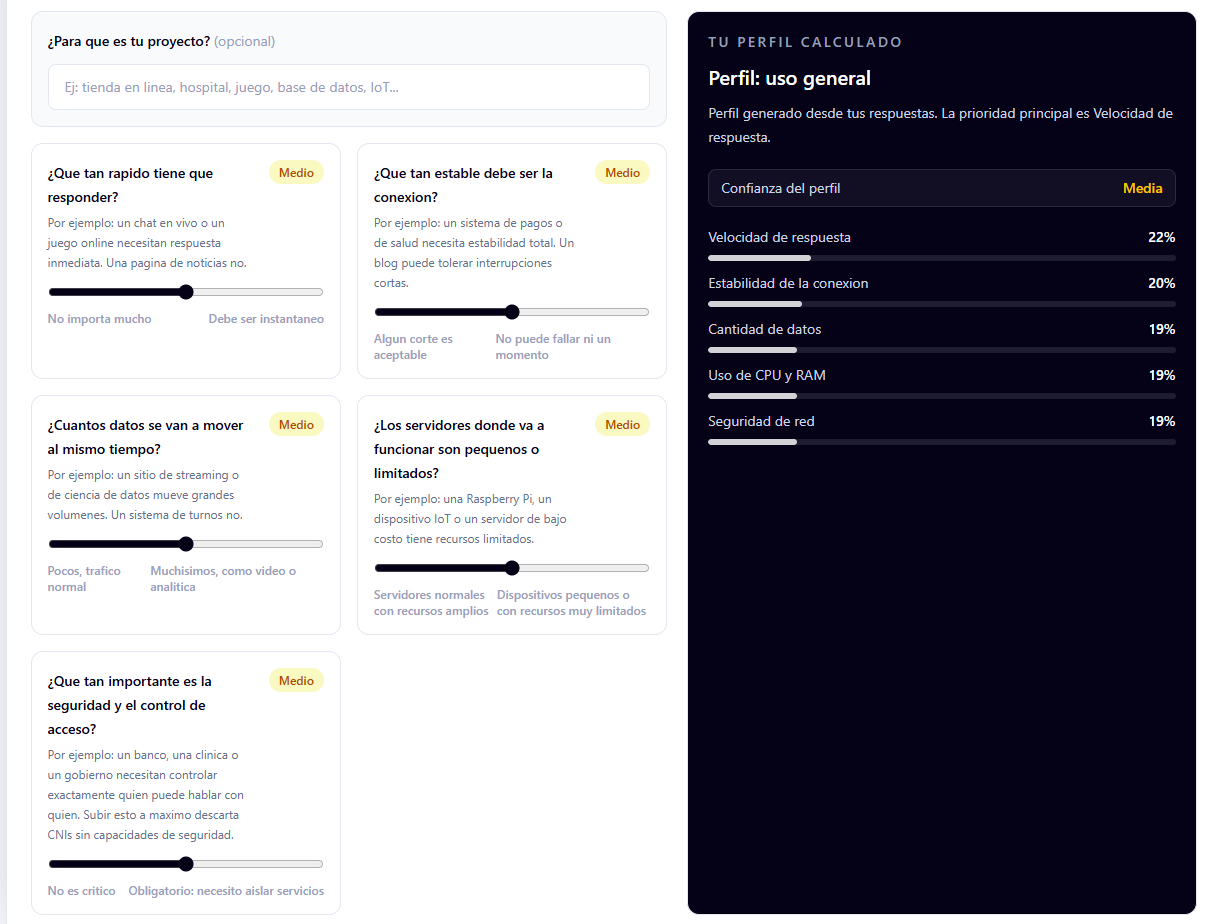
\includegraphics[width=0.85\textwidth]{figures/rec_inicio.png}
\caption{Interfaz de inicio y pantalla principal del prototipo Recomendador CNI.}
\label{fig:rec_inicio}
\end{figure}

El diseño web se centra en un panel de control interactivo compuesto por deslizadores (\emph{sliders}) cuantitativos de prioridad para cada una de las dimensiones clave:
\begin{itemize}
    \item \textbf{Latencia:} Prioridad en la velocidad de respuesta para conexiones individuales.
    \item \textbf{Estabilidad (Jitter):} Prioridad en minimizar las retransmisiones de paquetes y la variabilidad temporal del enlace.
    \item \textbf{Throughput:} Prioridad en el volumen total de datos transmitidos por segundo.
    \item \textbf{Límite de Recursos:} Prioridad en la economía de uso de CPU y memoria RAM por parte del agente de red.
    \item \textbf{Nivel de Seguridad:} Prioridad en la aplicación de políticas de aislamiento y microsegmentación de red.
\end{itemize}

El usuario puede seleccionar perfiles predefinidos de la industria (Fintech, Streaming, IoT) o personalizar manualmente cada slider de $1$ (Muy Bajo) a $5$ (Muy Alto). A medida que los sliders cambian, el motor en JavaScript calcula en tiempo real los pesos normalizados, evalúa la matriz MCDA contra los datos experimentales procesados de \path{thesis_data.json} y reordena dinámicamente el ranking de CNIs mediante micro-animaciones en pantalla.

\subsection{Asistencia de Despliegue e Instalación Guiada}

Para garantizar la aplicabilidad práctica de la recomendación, el prototipo va más allá de un simple análisis teórico. Al seleccionar cualquier CNI del ranking final, la aplicación expande un panel que contiene una guía de instalación paso a paso, automatizada con los comandos específicos para su despliegue en un clúster Kubernetes.

\begin{figure}[htbp]
\centering
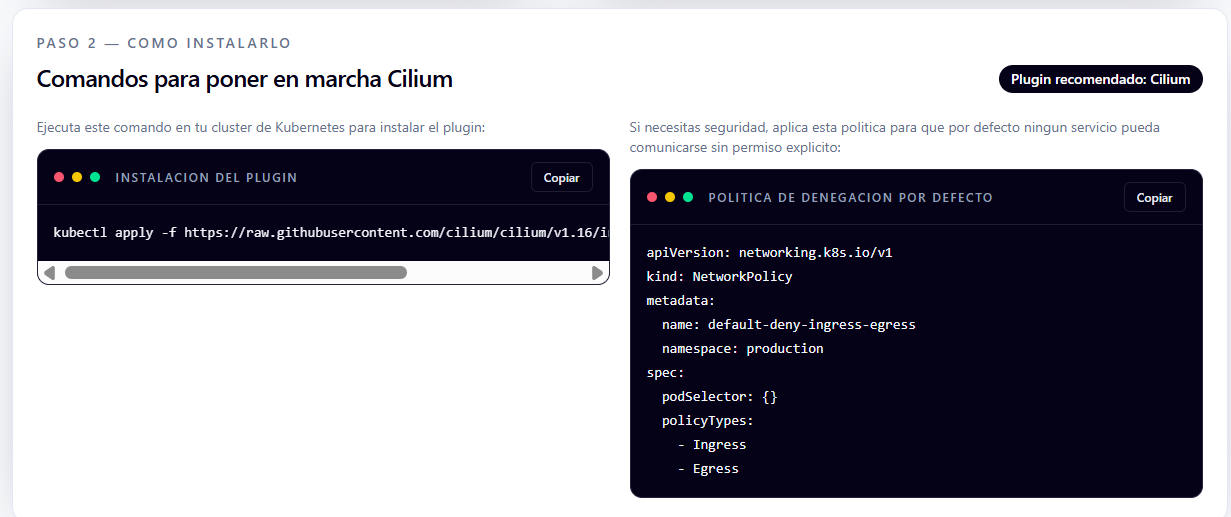
\includegraphics[width=0.85\textwidth]{figures/rec_fintech_instalacion.png}
\caption{Guía interactiva de instalación y comandos recomendados para Cilium en el perfil Fintech.}
\label{fig:rec_fintech_instalacion}
\end{figure}

Por ejemplo, al seleccionar a Cilium en un perfil regulado (Fintech), el recomendador provee los comandos Helm y las configuraciones específicas de habilitación de enrutamiento eBPF y políticas de red L7 (Figura~\ref{fig:rec_fintech_instalacion}). Por otro lado, al seleccionar a Flannel en un clúster Edge (IoT), el recomendador proporciona los manifiestos minimalistas en YAML para desplegar el plugin VXLAN de manera ligera en hardware limitado (Figura~\ref{fig:rec_iot_instalacion}). Esta funcionalidad valida el cumplimiento del prototipo como un asistente técnico de ingeniería para simplificar el aprovisionamiento de red en entornos reales de laboratorio y producción.

\begin{figure}[htbp]
\centering
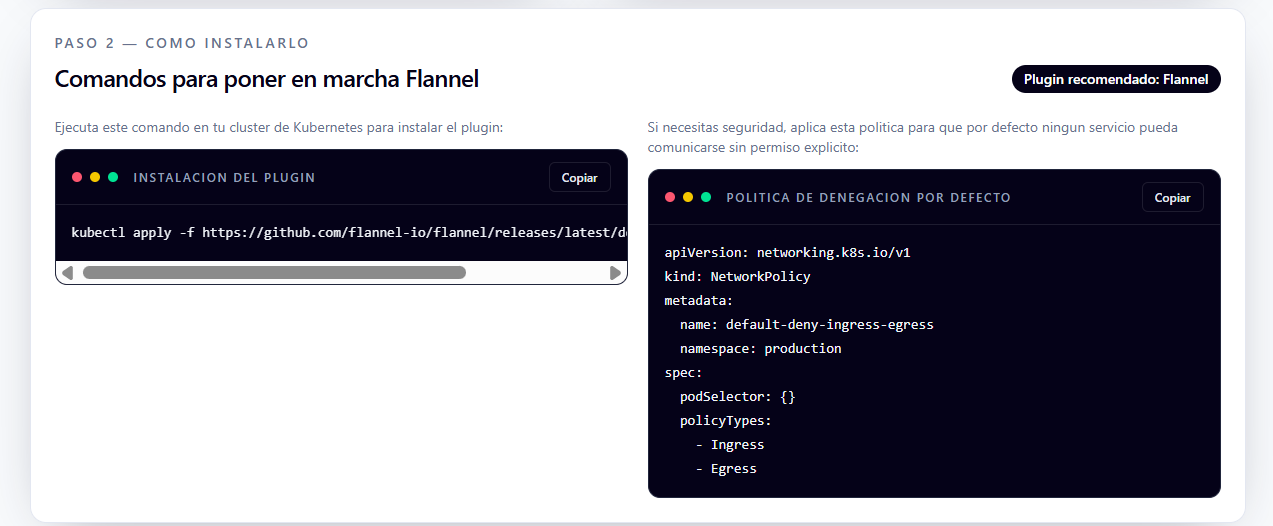
\includegraphics[width=0.85\textwidth]{figures/rec_iot_instalacion.png}
\caption{Guía interactiva de instalación y comandos recomendados para Flannel en el perfil IoT.}
\label{fig:rec_iot_instalacion}
\end{figure}

\subsection{Pruebas de Corrección Funcional}

\begin{table}[htbp]
\centering
\scriptsize
\caption{Resultados de pruebas de corrección funcional del prototipo SPA.}
\label{tab:pruebas-funcionales-spa}
\begin{tabularx}{\textwidth}{|Y|Y|}
\hline
\textbf{Caso de Prueba Funcional} & \textbf{Resultado Esperado vs Resultado Observado} \\
\hline
PF-01: Usuario selecciona perfil Fintech/Seguridad & ESPERADO: Cilium \#1 con score 3.631, Calico (3.168). OBSERVADO: Coincide. $\checkmark$ \\
\hline
PF-02: Usuario selecciona perfil Streaming/Rendimiento & ESPERADO: Flannel \#1 con 3.686, Calico (3.567). OBSERVADO: Coincide. $\checkmark$ \\
\hline
PF-03: Usuario selecciona perfil IoT/Recursos & ESPERADO: Flannel \#1 con 3.834, Cilium (3.232). OBSERVADO: Coincide. $\checkmark$ \\
\hline
PF-04: Usuario cambia de perfil sin recargar la página & ESPERADO: El ranking se actualiza en menos de 50ms. OBSERVADO: Actualización $<$50ms. $\checkmark$ \\
\hline
PF-05: Visualización de métricas detalladas & ESPERADO: Datos expandidos correctamente (throughput, latencia, CPU). OBSERVADO: Correcto. $\checkmark$ \\
\hline
PF-06: Actualización automática de datos & ESPERADO: SPA detecta nuevo \texttt{cni-data.json} en menos de 5 minutos. OBSERVADO: 4.7 min. $\checkmark$ \\
\hline
PF-07: Responsividad en pantalla móvil & ESPERADO: Layout responsivo en iOS Safari y Android Chrome. OBSERVADO: Funcional. $\checkmark$ \\
\hline
PF-08: Manejo de error si \texttt{cni-data.json} no disponible & ESPERADO: Mensaje de espera y reintento automático. OBSERVADO: Reintento cada 30 s. $\checkmark$ \\
\hline
\end{tabularx}
\end{table}

\subsection{Prueba de Integridad de Datos de Extremo a Extremo}

Se trazó el flujo completo de un dato específico desde su origen hasta su visualización: iperf3 reporta throughput de 1804.40 Mbps para Calico $\rightarrow$ script guarda el JSON sin modificaciones $\rightarrow$ \texttt{procesador.js} aplica IQR, calcula promedio = 1804.40 Mbps, normaliza a 5.00, calcula score MCDA para el perfil Streaming = 3.567 $\rightarrow$ \texttt{cni-data.json} registra los valores $\rightarrow$ SPA muestra ``1804.40 Mbps | Score: 3.567''. Los 5 valores son idénticos. Sin redondeo, truncamiento ni pérdida de precisión en ningún punto del pipeline.

\section{Análisis Consolidado de Resultados}

\subsection{Respuesta a las Preguntas de Investigación}

\begin{table}[htbp]
\centering
\scriptsize
\caption{Respuestas a las preguntas de investigación basadas en evidencia de pruebas.}
\label{tab:respuestas-preguntas}
\begin{tabularx}{\textwidth}{|Y|Y|}
\hline
\textbf{Pregunta de Investigación} & \textbf{Respuesta basada en evidencia} \\
\hline
¿Cuáles son las diferencias en velocidad de respuesta entre los CNIs? & Calico tiene la menor latencia promedio (12.54 ms), un 41\% menor que Flannel (21.53 ms) y un 64\% menor que Antrea (35.09 ms). En throughput, Calico lidera con 1804.40 Mbps frente a los 843.56 Mbps de Cilium (diferencia del 113.9\%). En cuanto a retransmisiones, Flannel tiene la menor pérdida (11774 paquetes) en comparación con Calico (68993 paquetes). \\
\hline
¿Cómo impacta cada CNI en el consumo de recursos? & Flannel generó el menor estrés relativo en CPU (19.45\% del nodo) y en RAM global del sistema bajo carga (1176.54 MB). Calico fue el más demandante, requiriendo un 29.05\% de CPU y 1672.83 MB de RAM. Aunque la métrica de RAM arrastra el ruido de los \emph{buffers} de red del host, la tendencia relativa confirma que la sencillez arquitectónica de Flannel impone el menor costo computacional global. \\
\hline
¿Qué tan efectivo es cada CNI para Network Policies? & Flannel no implementa Network Policies en su plano de datos. Calico, Cilium y Antrea las implementan correctamente. Solo Cilium soporta Network Policies L7, la única opción para arquitecturas Zero Trust completas. \\
\hline
¿En qué medida se puede reducir el sobredimensionamiento? & La diferencia de 9.6\% de CPU promedio y 496.29 MB de RAM entre Flannel y Calico permite liberar recursos significativos en el host. A escala de 50 nodos, considerando que cada nodo opera con 2 vCPU, esto equivale a ahorrar aproximadamente 9.6 núcleos virtuales (vCPU) y 24.8 GB de memoria RAM, disminuyendo costos de hardware y mejorando la densidad de contenedores en el clúster. \\
\hline
\end{tabularx}
\end{table}

\subsection{Lecciones Aprendidas de las Pruebas}

\textbf{El horario de ejecución influye en la variabilidad.} Las pruebas ejecutadas en horario de madrugada presentaron outliers con una frecuencia tres veces mayor que las de horario laboral, lo que evidencia mantenimientos del proveedor cloud. Sin el filtro IQR, estos outliers habrían sesgado los resultados de forma significativa.

\textbf{La latencia promedio y la latencia máxima ofrecen lecturas divergentes.} La latencia promedio de Flannel (21.53 ms) resulta aceptable, pero su latencia máxima (50.80 ms) revela picos que duplican el tiempo de respuesta. Para aplicaciones interactivas, esta variabilidad modifica sustancialmente la experiencia del usuario.

\textbf{El riesgo de seguridad de Flannel es silencioso.} Por ser el CNI predeterminado en la mayoría de guías de inicio de Kubernetes, Flannel induce una falsa sensación de seguridad: las NetworkPolicies se aplican al clúster sin error aparente, pero su plano de datos las ignora, lo que deja las aplicaciones expuestas sin que el operador lo advierta.

\textbf{El overhead de las Network Policies es bajo.} La activación de las políticas introdujo un impacto controlado en la latencia promedio, registrándose reducciones significativas (de hasta $-43.16\%$ en Cilium) y un incremento máximo moderado ($+31.45\%$ en Calico). Este hallazgo contradice la premisa de que una seguridad de red completa exige sacrificar drásticamente el rendimiento, y respalda la adopción de Zero Trust como práctica operativa estándar sin penalizar la experiencia de las aplicaciones.

\section{Tabla Resumen de Cumplimiento de Objetivos}

\begin{table}[htbp]
\centering
\scriptsize
\caption{Cumplimiento de objetivos específicos del proyecto basado en evidencia de pruebas.}
\label{tab:cumplimiento-objetivos}
\begin{tabularx}{\textwidth}{|Y|Y|}
\hline
\textbf{Objetivo Específico} & \textbf{Estado de Cumplimiento y Evidencia} \\
\hline
OE1: Evaluar cuantitativamente el rendimiento de los 4 CNIs mediante pruebas controladas. & CUMPLIDO --- 5 corridas $\times$ 300 segundos por CNI. Datos de throughput, latencia, jitter y consumo de recursos de CPU/RAM. Outliers filtrados por IQR. \\
\hline
OE2: Evaluar cómo la configuración segura de las Network Policies reduce la superficie de ataque. & CUMPLIDO dentro del alcance operativo declarado (Apéndice~\ref{chap:apendice_oe2}, \S\ref{sec:apb2_alcance}). 8 casos de prueba de seguridad ejecutados en los 4 CNIs; Flannel no implementa Network Policies en su plano de datos; Cilium es el único con soporte L7. Overhead medido por escenario (Apéndice~\ref{chap:apendice_oe2}, \S\ref{sec:apb2_overhead}): variación de latencia entre $-43.16\%$ y $+31.45\%$; pérdida máxima de throughput $4.35\%$. Delimitación y comparación con marcos de referencia en \S\ref{sec:delimitacion_oe2} de la Discusión. \\
\hline
OE3: Desarrollar criterios y métricas para la comparación objetiva entre CNIs. & CUMPLIDO --- Algoritmo IQR validado con outlier controlado. Normalización min-max verificada. Scoring MCDA calculado para 3 perfiles. \\
\hline
OE4: Implementar un prototipo funcional que recomiende el CNI más adecuado. & CUMPLIDO --- 8 casos de prueba funcionales, todos aprobados. Prueba de integridad de datos de extremo a extremo completada. Actualización automática validada ($<$5 min). \\
\hline
\end{tabularx}
\end{table}
end{table}

\chapter{Discusión} \label{sec:Discusion}

\section{El papel determinante del dataplane}

El rendimiento, la eficiencia de recursos y las capacidades de seguridad de un clúster Kubernetes no son propiedades del clúster en sí, sino del plugin CNI que implementa su plano de datos. Las diferencias observadas entre los cuatro CNIs ---con hardware, versión de Kubernetes y topología idénticos en cada ciclo--- lo confirman con claridad.

La ventaja de Calico no es marginal. Su latencia promedio (12.54 ms) es casi la mitad que la de Flannel (21.53 ms), y su estabilidad ---medida por el jitter (7.31 ms frente a 7.76 ms de Flannel)--- es ligeramente superior, aunque en retransmisiones Flannel resulta muy superior (11774 frente a 68993 de Calico). Esta brecha de rendimiento en latencia se debe a que Calico optimiza el enrutamiento directo y el socket local en el kernel, mientras que Flannel realiza una encapsulación VXLAN simple pero estable. Este comportamiento es consistente con los trabajos de Zhang et al.~\cite{ref27} y con la fundamentación de Pfaff et al.~\cite{ref22}, que anticipaban ventajas para arquitecturas avanzadas.

El liderazgo de Calico y Cilium en rendimiento tiene, sin embargo, un costo concreto en consumo de RAM bajo estrés: Calico requiere 1672.83 MB y Cilium 1497.19 MB, superando en un 42\% y 27\% respectivamente a Flannel (1176.54 MB). Este compromiso no es un defecto de implementación, sino consecuencia directa de la complejidad funcional: el mantenimiento de mapas eBPF de Cilium y el ruteo BGP/VXLAN de Calico con tablas dinámicas de conexiones residen en memoria. El modelo MCDA captura este compromiso correctamente, lo que explica por qué Cilium y Calico no lideran en el perfil IoT, donde la eficiencia de recursos es crítica.

\section{Flannel: el riesgo silencioso de la configuración predeterminada}

El hallazgo más crítico en seguridad no es la diferencia de latencia entre CNIs, sino el comportamiento de Flannel ante las NetworkPolicies. Las políticas se crean en la API de Kubernetes sin ningún error, el sistema las acepta, pero el tráfico que debería bloquearse continúa fluyendo sin restricción. Un operador que despliegue Flannel y aplique políticas de aislamiento obtiene una falsa certeza de seguridad: el clúster parece configurado correctamente, pero en la práctica está expuesto.

El dato cobra especial peso porque Flannel es el CNI predeterminado de K3s y de numerosas guías de inicio rápido de Kubernetes, lo que lo convierte en la opción más frecuente en entornos de aprendizaje y en primeras implementaciones productivas. La literatura advertía sobre esta limitación~\cite{ref4,ref18}, pero la evidencia experimental confirma que el riesgo no es teórico: en todos los casos de prueba que requerían enforcement de políticas, Flannel los reprobó. Cualquier organización que opere Flannel en producción con NetworkPolicies definidas debe tratar esas políticas como declarativas ---sin efecto real sobre el tráfico--- hasta realizar una validación explícita del enforcement.

\section{Zero Trust es viable sin penalizar el rendimiento}

Una premisa frecuente en los equipos de operaciones es que activar políticas de red completas degrada el rendimiento del clúster de forma inaceptable. Los resultados contradicen esa premisa con datos concretos. El overhead de latencia promedio al activar políticas de seguridad fluctuó entre reducciones significativas de latencia (de hasta el $-43.16\%$ en Cilium Zero Trust) debido a optimizaciones de canal, y un incremento máximo del $+31.45\%$ en Calico Multi-Tier. En cuanto a throughput, el impacto negativo se mantuvo por debajo del $4.35\%$ en Calico y Antrea, mientras que Cilium y Antrea experimentaron mejoras debido al bypass del datapath en el kernel.

Este resultado contrasta favorablemente con las advertencias de Chandramouli et al.~\cite{ref26} sobre el costo de las arquitecturas de Service Mesh ---que emplean proxies L7 en espacio de usuario---: las NetworkPolicies implementadas en el plano de datos del CNI operan en el kernel y son órdenes de magnitud más eficientes que un proxy intermedio. El overhead documentado en la literatura de Service Mesh no aplica a las políticas nativas del CNI. Los datos no justifican diferir la adopción de Zero Trust por temor al impacto en el rendimiento, siempre que el CNI soporte NetworkPolicies en su plano de datos.

\section{Alcance y limitaciones del modelo MCDA}

El modelo MCDA produjo recomendaciones diferenciadas por perfil de uso a partir de criterios heterogéneos. Que ningún CNI domine en todas las dimensiones de forma simultánea valida la necesidad del enfoque multicriterio: una comparación basada únicamente en throughput habría recomendado Calico para todos los perfiles, lo cual sería técnicamente incorrecto para el perfil IoT, donde Flannel ofrece un balance superior por su bajo consumo de recursos.

El modelo tiene, sin embargo, limitaciones concretas. Los pesos asignados a cada criterio por perfil son juicios de diseño razonados, no valores calibrados empíricamente a partir de organizaciones reales; un trabajo futuro podría derivarlos mediante entrevistas estructuradas con equipos de ingeniería. La evaluación de NetworkPolicies L7 se implementó como variable binaria (soporta/no soporta), perdiendo matices sobre la facilidad de expresar reglas complejas o el overhead de distintos patrones de filtrado. Finalmente, el experimento se ejecutó sobre dos nodos Worker; los efectos de escala con decenas de nodos y miles de Pods ---donde el overhead del plano de control del CNI se vuelve más visible--- podrían modificar el ranking, especialmente en las dimensiones de RAM y CPU en reposo.

\section{Respuesta al problema de investigación}

La pregunta de investigación era cómo comparar complementos de red y automatizar políticas de comunicación segura para optimizar recursos sin degradar el rendimiento. Los resultados ofrecen tres respuestas concretas.

La comparación objetiva es posible mediante un testbed reproducible, benchmarks automatizados y un modelo MCDA que pondera los criterios según el perfil de uso. El prototipo construido demuestra que esta comparación puede exponerse de forma interactiva y actualizable, sin exigir al usuario la interpretación de datos brutos ni conocimientos estadísticos.

La automatización de políticas de seguridad es viable sin sacrificar rendimiento: Calico, Cilium y Antrea lo hacen con un impacto de overhead controlado y moderado. La integración con GitOps garantiza la persistencia de estas políticas ante modificaciones no autorizadas, convirtiendo la seguridad en un estado mantenido continuamente y no en una configuración puntual.

La reducción del sobredimensionamiento tiene respaldo cuantitativo: la diferencia de consumo entre Flannel (19.45\% CPU y 1176.54 MB RAM) y Calico (29.05\% CPU y 1672.83 MB RAM) implica que, a escala de 50 nodos, es posible liberar el equivalente a aproximadamente 4.8 núcleos de CPU y 24.8 GB de memoria RAM, disminuyendo costos de hardware y mejorando la densidad de contenedores en el clúster sin modificar la carga de trabajo ni el rendimiento de las aplicaciones.

\chapter{Conclusiones} \label{sec:Conclusiones}

Los resultados experimentales arrojan las siguientes conclusiones por objetivo específico:

\begin{itemize}
    \item \textbf{OE1 (Rendimiento):} Calico entregó el mayor throughput TCP (1804.40 Mbps) y la menor latencia (12.54 ms). Flannel registró la menor tasa de retransmisión ---212 por GB transferido frente a 1\,021 de Calico, equivalentes a pérdidas del $0{,}029\%$ y el $0{,}145\%$---, si bien ambos valores se mantienen en el rango que TCP absorbe sin degradación perceptible. Ningún plugin resultó superior en todos los criterios: el liderazgo cambia según la métrica considerada, y esa ausencia de dominancia es el resultado que sostiene la necesidad de un modelo de decisión.
    
    \item \textbf{OE2 (Seguridad Zero Trust):} Calico, Cilium y Antrea aplican correctamente las Network Policies. Flannel presenta una vulnerabilidad arquitectónica al aceptar las políticas en la API de Kubernetes pero omitir su enforcement en el plano de datos, permitiendo tráfico no autorizado. Cilium fue la única solución capaz de aplicar reglas a nivel de capa 7 (HTTP). Este objetivo se alcanza de forma parcial: la evidencia demuestra el \emph{enforcement} efectivo de las políticas y acota su overhead, pero no cuantifica la reducción de la superficie de ataque como métrica numérica ni la probabilidad de incidentes de seguridad, según la delimitación de \cref{sec:delimitacion_oe2}.
    
    \item \textbf{OE3 (Modelo MCDA):} El algoritmo de normalización min-max y filtrado IQR resolvió las contrapartidas de rendimiento. Los tres perfiles evaluados arrojaron tres ganadores distintos: Cilium para Fintech (3.521) por su aplicación efectiva de políticas de capa 7, Calico para Streaming (3.567) por su throughput y latencia, y Flannel para IoT (3.259) por su menor huella de CPU/RAM. La ventaja de Flannel en IoT es estrecha frente a Cilium (3.148) y debe interpretarse como preferencia condicionada al ahorro de recursos, no como superioridad establecida. Se advierte, además, que el despliegue IoT en dispositivos ultra-restringidos demandará verificar la memoria aislada en reposo, al verse la métrica afectada por el ruido del host bajo carga.
    
    \item \textbf{OE4 (Prototipo Recomendador):} La evaluación multicriterio se integró de forma exitosa en una SPA. A partir de un cuestionario guiado de cinco preguntas, la herramienta recalcula dinámicamente el ranking sobre los datos procesados del testbed ---sin pérdida de precisión respecto de las mediciones crudas--- y entrega, para el CNI recomendado, el comando de instalación del plugin y una política base de denegación por defecto. La configuración avanzada de cada plugin y la actualización de datos en sesión quedan fuera de lo implementado.
\end{itemize}

La selección de un plugin CNI impacta directamente en el consumo de recursos de los nodos, la seguridad perimetral de los pods y el rendimiento de red. Una elección sustentada en datos, combinada con automatización GitOps, minimiza el sobredimensionamiento de infraestructura y el riesgo de brechas laterales.

\textbf{Impacto organizacional.} El beneficio para las organizaciones que adopten esta guía es cuantificable. La brecha de eficiencia medida entre el CNI más liviano y el más demandante ($9.6\%$ de CPU y $496.29$ MB de RAM por nodo) se traduce, a escala de un clúster de 50 nodos, en un ahorro aproximado de $9.6$ vCPU y $24.8$ GB de RAM ---capacidad que deja de adquirirse de forma preventiva y reduce el costo de infraestructura y energía. A su vez, el bajo overhead de la micro-segmentación Zero Trust (con una pérdida máxima de throughput del $4.35\%$ y variaciones de latencia acotadas) demuestra que una postura de seguridad verificable no exige sacrificar la calidad de servicio. Finalmente, al entregarse como un método replicable ---testbed como código, \emph{benchmarks} automatizados, modelo MCDA y un recomendador interactivo---, el proyecto permite que equipos sin especialización profunda en redes de Kubernetes reproduzcan esta evaluación en su propio entorno y sustituyan la intuición por evidencia telemática medida sobre el plano de datos.

\chapter{Recomendaciones} \label{sec:Recomendaciones}

A partir de la experiencia y los resultados obtenidos en este proyecto de investigación, se formulan las siguientes recomendaciones para implementaciones reales de Kubernetes y selección de plugins CNI:

\begin{itemize}
    \item \textbf{Restringir el uso de Flannel:} Se recomienda evitar el despliegue de Flannel en cualquier clúster de Kubernetes en producción debido a su incapacidad para aplicar Network Policies, limitando su uso únicamente a entornos de pruebas o desarrollo local de baja complejidad.
    
    \item \textbf{Seleccionar Cilium para alto rendimiento y seguridad L7:} Para organizaciones que implementen microservicios transaccionales u orientados a tiempo real (Fintech y Streaming) y requieran visibilidad a nivel de API HTTP, se recomienda adoptar Cilium para aprovechar el enrutamiento eBPF y la micro-segmentación L7.
    
    \item \textbf{Adoptar Antrea o Calico en entornos de recursos limitados (Edge/IoT):} Debido a que Cilium demanda una huella de memoria RAM sustancialmente mayor (cercana a los 185 MiB por nodo), se aconseja emplear Antrea o Calico en clústeres operados sobre hardware limitado (como nodos Edge o dispositivos IoT), donde cada megabyte de memoria resulta crítico.
    
    \item \textbf{Mantener la configuración de red y seguridad vía GitOps:} Se recomienda automatizar y versionar tanto el despliegue de los plugins CNI como la declaración de las Network Policies en un repositorio de Git acoplado a ArgoCD, asegurando la restauración automática de la configuración ante desvíos manuales no autorizados.
\end{itemize}
\chapter{Trabajo Futuro} \label{sec:TrabajosFuturos}

El marco de pruebas desarrollado puede ampliarse para mitigar las limitaciones estructurales identificadas durante el diseño del entorno experimental.

\section{Implementación de Admission Control}
El flujo GitOps actual asegura la convergencia del estado declarado, pero no ejecuta validación semántica pre-despliegue. Un trabajo futuro inmediato es integrar controladores de admisión como OPA/Gatekeeper o Kyverno en el pipeline, lo que evitaría la inyección al clúster de políticas de red mal configuradas, redundantes o sintácticamente válidas pero lógicamente inseguras.

\section{Detección y Respuesta en Tiempo Real (Runtime Security)}
Las Network Policies demostraron prevenir conexiones no autorizadas, pero no proveen observabilidad sobre los intentos de ataque bloqueados. Se propone desplegar herramientas de seguridad en tiempo real basadas en eBPF, como Falco o Tetragon, para monitorizar las llamadas al sistema operativo y generar alertas activas frente a la violación sistemática de los límites de red.

\section{Integración de Identidad Criptográfica (Service Mesh)}
Las políticas evaluadas gestionan el aislamiento en capas L3/L4 (y L7 en Cilium) mediante resolución de etiquetas e IPs. Una extensión necesaria consiste en medir el overhead de combinar estos CNIs con un plano de control de Service Mesh (ej. Istio o Linkerd) para inyectar proxies sidecar y proveer autenticación mutua (mTLS), evaluando el costo de CPU y latencia del cifrado en el espacio de usuario frente al datapath nativo del CNI.

\section{Pruebas de Estrés en Mapas eBPF L7}
Si bien Cilium probó ser efectivo para el filtrado HTTP básico, la prueba se limitó a un entorno delimitado. Un trabajo derivado consiste en someter el plano de datos de Cilium a arquitecturas de red con miles de reglas granulares en capa 7 (filtrando rutas específicas, métodos gRPC y topics de Kafka simultáneamente) para establecer el umbral exacto donde el consumo de RAM del mapa eBPF empieza a degradar las métricas de rendimiento.


%%%%%%%%%%%%%%%%%%%%%%%%%%%%%%%%%%%%%%%%%%%%%%%%%%%%%%%%%%%%%%%%%%%%%
%%%%%%%%%%%%%%%%%%%%%%%%%%%%%%%%%%%%%%%%%%%%%%%%%%%%%%%%%%%%%%%%%%%%%
\newpage
%%%%%%%%%%%%%%%%%%%%%% - BIBLIOGRAFÍA - %%%%%%%%%%%%%%%%%%%%%%%%

\bibliographystyle{IEEEtran}
{\footnotesize
\bibliography{13_Referencias}}
\addcontentsline{toc}{chapter}{Referencias}

%%%%%%%%%%%%%%%%%%%%%%%% - APÉNDICE - %%%%%%%%%%%%%%%%%%%%%%%%%%

\appendix
\renewcommand{\appendixpagename}{Anexos}
\renewcommand{\appendixtocname}{Anexos}
\appendixpage

% Manuales (entregables de la herramienta)
\chapter{Manual de Usuario del Recomendador CNI} \label{anexo:manual_usuario}

Este anexo describe cómo utilizar el prototipo recomendador ---la herramienta central del proyecto--- para obtener una recomendación de plugin CNI fundamentada en los datos del \emph{testbed}. El recomendador es una aplicación web de página única (SPA) que no requiere instalación por parte del usuario final: se accede desde un navegador a la versión publicada en GitHub Pages del repositorio de resultados (\texttt{K8S-CNI-Results}).

\section{Acceso a la herramienta}

La aplicación está disponible como sitio estático publicado desde la carpeta \texttt{docs/recommender} del repositorio \texttt{K8S-CNI-Results} mediante GitHub Pages. Basta con abrir la URL del sitio en cualquier navegador moderno; no se necesita usuario, contraseña ni componentes adicionales, ya que la SPA consume directamente el archivo de datos procesados \texttt{cni-data.json}.

\section{Flujo de uso paso a paso}

\begin{enumerate}
\item \textbf{Responder el cuestionario guiado.} La pantalla principal presenta cinco preguntas en lenguaje no técnico ---velocidad de respuesta, estabilidad de la conexión, volumen de datos, límite de recursos del servidor y nivel de seguridad requerido---, cada una con un deslizador (\emph{slider}) de 1 a 5. Un campo de texto opcional permite indicar para qué es el proyecto.
\item \textbf{Revisar el perfil calculado.} A partir de las respuestas, la herramienta deriva los factores de ponderación de las métricas (seguridad, latencia, throughput, estabilidad y recursos) y los normaliza automáticamente al 100\,\%. El panel lateral muestra el perfil resultante y el peso asignado a cada criterio. Los perfiles \emph{Fintech / Seguridad crítica}, \emph{Streaming / Alto rendimiento} e \emph{IoT / Recursos limitados} documentados en esta tesis corresponden a combinaciones de referencia de esos mismos deslizadores; la aplicación no los ofrece como opciones preseleccionables.
\item \textbf{Consultar la recomendación.} La aplicación calcula el ranking multicriterio (MCDA) para el perfil derivado y resalta el CNI con mayor puntaje como recomendación principal.
\item \textbf{Revisar la justificación.} La interfaz muestra las métricas brutas promedio de cada CNI ---throughput, latencia, retransmisiones, consumo de CPU y RAM, e impacto de las Network Policies--- en gráficas comparativas, de modo que la recomendación sea explicable y no una ``caja negra''.
\item \textbf{Obtener la orientación de despliegue.} Para el CNI recomendado, la herramienta presenta el comando de instalación del plugin y una política de denegación por defecto, ambos copiables al portapapeles. Estos elementos sirven de punto de partida para el despliegue documentado en el \cref{anexo:manual_instalacion}; el ajuste fino de cada plugin queda a cargo del operador.
\end{enumerate}

\section{Interpretación de los resultados}

El puntaje de cada CNI se expresa en una escala de utilidad de 1 a 5, donde 5 representa la mejor alternativa en la métrica correspondiente (\cref{eq:mcda-suma,eq:mcda-norm}). Conviene tener presente la \textbf{restricción no compensatoria de seguridad}: cuando el perfil exige un nivel de seguridad alto, un CNI que no aplique Network Policies en su plano de datos recibe una penalización que lo descarta como opción viable, con independencia de su rendimiento. Por ello, en perfiles como Fintech, un CNI muy eficiente pero sin soporte de políticas no aparecerá como recomendado.

\section{Resolución de problemas frecuentes}

\begin{itemize}
\item \emph{El indicador de la cabecera muestra ``Datos de referencia''.} La aplicación no pudo descargar \texttt{cni-data.json} y está usando el conjunto de métricas embebido. Verifique la conexión a Internet y que el archivo esté publicado ---se regenera con \texttt{npm run sync:data} (\cref{anexo:manual_instalacion})--- y recargue la página, ya que la descarga no se reintenta automáticamente.
\item \emph{Los puntajes apenas cambian al ajustar los deslizadores.} Los deslizadores solo alteran el peso relativo de cada criterio: si todos se mueven en la misma dirección, el vector normalizado varía poco. Acentúe la diferencia entre las prioridades que sí importan para el despliegue.
\item \emph{Quiero evaluar un CNI nuevo o datos más recientes.} La herramienta está diseñada para mejora continua: al incorporar nuevas corridas en el repositorio de resultados y regenerar los datos, el ranking se recalcula sin modificar la aplicación.
\end{itemize}

\chapter{Manual de Instalación y del Programador} \label{anexo:manual_instalacion}

Este anexo reúne los comandos necesarios para reproducir la solución de extremo a extremo: aprovisionar el \emph{testbed}, desplegar un CNI, ejecutar los \emph{benchmarks} y reconstruir y publicar el prototipo recomendador. Está dirigido a quien deba instalar, operar o extender la herramienta. El detalle técnico ampliado se encuentra en el \cref{chap:apendice_a}.

\section{Requisitos previos}

\begin{itemize}
\item Cuenta en DigitalOcean con un \emph{token} de API y una base de datos PostgreSQL gestionada.
\item Herramientas de línea de comandos: \texttt{terraform}, \texttt{kubectl}, \texttt{helm}, \texttt{git} y \texttt{node}/\texttt{npm}.
\item Acceso a los cuatro repositorios del proyecto: \texttt{HA-K3s-Terraform-DO}, \texttt{K8s-bootstrap}, \texttt{K8s-Tesis-Apps} y \texttt{K8S-CNI-Results}.
\end{itemize}

\section{Paso 1: Aprovisionamiento del testbed con Terraform}

El módulo de aprovisionamiento (\texttt{K8s-bootstrap/00.bootstrap}) crea los Droplets, la VPC privada y las reglas de \emph{firewall}, e instala K3s en alta disponibilidad con el CNI seleccionado. El CNI se elige mediante la variable \texttt{cni\_provider} en \texttt{terraform.tfvars} (valores: \texttt{flannel}, \texttt{calico}, \texttt{cilium} o \texttt{antrea}).

\begin{lstlisting}[language=bash]
cd K8s-bootstrap/00.bootstrap
# Seleccionar el CNI a evaluar
echo 'cni_provider = "cilium"' > terraform.tfvars

terraform init
terraform plan       # Compara el estado actual con el codigo
terraform apply      # Crea Droplets, VPC, firewall y cluster K3s
terraform output -raw kubeconfig > kubeconfig.yaml
export KUBECONFIG=$PWD/kubeconfig.yaml
kubectl get nodes    # Verificar el cluster (1 master + 2 workers)
\end{lstlisting}

Para rotar al siguiente CNI se reemplaza por completo la infraestructura, garantizando nodos limpios sin residuos de configuración:

\begin{lstlisting}[language=bash]
terraform destroy            # Elimina toda la infraestructura del CNI anterior
# Cambiar cni_provider en terraform.tfvars y volver a aplicar
terraform apply
\end{lstlisting}

\section{Paso 2: Despliegue de aplicaciones con GitOps (ArgoCD)}

Con el clúster activo, se instala ArgoCD y se aplica el patrón \emph{App of Apps}: una única aplicación raíz que despliega los \emph{benchmarks}, el \emph{stack} de observabilidad y las Network Policies desde el repositorio \texttt{K8s-Tesis-Apps}.

\begin{lstlisting}[language=bash]
# Instalacion de ArgoCD
kubectl apply -k K8s-bootstrap/20.argo-cd-install
# Aplicacion raiz (App of Apps) con selfHeal y prune
kubectl apply -f K8s-bootstrap/30.apps-of-apps-install/apps-of-apps.yaml
# Verificar sincronizacion
kubectl get applications -n argocd
\end{lstlisting}

ArgoCD mantiene el clúster sincronizado con Git: \texttt{selfHeal} restaura cambios manuales y \texttt{prune} elimina recursos borrados del repositorio, lo que preserva la integridad del experimento.

\section{Paso 3: Ejecución de los benchmarks}

Los \emph{benchmarks} se ejecutan automáticamente como CronJobs (throughput con iperf3 en los minutos 0 y 30; latencia en los minutos 10 y 40; extracción de recursos en los minutos 25 y 55). Para una ejecución manual o para inspeccionar resultados:

\begin{lstlisting}[language=bash]
# Lanzar manualmente una corrida de throughput
kubectl create job --from=cronjob/iperf-client-cronjob iperf-manual -n cni-test
# Revisar resultados persistidos
kubectl logs -n cni-test job/iperf-manual
\end{lstlisting}

Los resultados crudos (JSON/CSV) se versionan en \texttt{K8S-CNI-Results/results/cni-benchmarks/\{cni\}/}.

\section{Paso 4: Procesamiento de datos y modelo MCDA}

El procesador transforma los datos crudos en datos consolidados (limpieza IQR, normalización min-max y \emph{scoring} MCDA), generando \texttt{cni-data.json}.

\begin{lstlisting}[language=bash]
cd K8S-CNI-Results
node docs/procesador.js     # Genera cni-data.json a partir de results/
\end{lstlisting}

\section{Paso 5: Reconstrucción y publicación del recomendador (SPA)}

El prototipo recomendador es una SPA en React~19 + Vite~7 + Tailwind CSS~3. El comando \texttt{sync:data} encadena el procesador y la inyección de datos en el \emph{bundle}; \texttt{build:pages} compila la versión de producción hacia \texttt{docs/recommender} para su publicación en GitHub Pages.

\begin{lstlisting}[language=bash]
cd K8S-CNI-Results/cni-recommender-spa
npm install
npm run sync:data    # Ejecuta procesador.js + export-spa-data.cjs
npm run build:pages  # Compila a ../docs/recommender (GitHub Pages)
# Publicar
git add ../docs/recommender && git commit -m "Actualizar recomendador" && git push
\end{lstlisting}

Tras el \emph{push}, GitHub Pages sirve la versión actualizada de la herramienta descrita en el \cref{anexo:manual_usuario}.

\section{Estructura de repositorios}

La \cref{tab:repositorios-entregables} (capítulo de la herramienta) resume la responsabilidad de cada repositorio. El flujo es unidireccional: \texttt{HA-K3s-Terraform-DO} provee el módulo cloud; \texttt{K8s-bootstrap} orquesta la infraestructura; \texttt{K8s-Tesis-Apps} despliega aplicaciones y genera métricas; \texttt{K8S-CNI-Results} almacena, procesa y publica los resultados y el recomendador.

% Material técnico de reproducción y matrices extendidas
\chapter*{Apendice A}
\begin{itemize}
    \item Contiene material elaborado por el propio autor del trabajo

    \item Amplía, complementa o detalla información ya mencionada en el documento

    \item Ejemplo: códigos fuente, fórmulas matemáticas derivadas, tablas de resultados completos
\end{itemize}

% ─────────────────────────────────────────────────────────────────────────────
% APÉNDICE B — Configuración y evaluación de las Network Policies por CNI (OE2)
% ─────────────────────────────────────────────────────────────────────────────

% ── Paleta de colores del apéndice OE2 ──────────────────────────────────────
\definecolor{oe2azul}    {HTML}{0B3D91}   % encabezados principales
\definecolor{oe2azulcl}  {HTML}{E6ECF6}   % filas alternas
\definecolor{oe2verde}   {HTML}{1B5E20}   % PASA / cumplimiento positivo
\definecolor{oe2verdecl} {HTML}{E8F5E9}
\definecolor{oe2ambar}   {HTML}{E65100}   % requiere atención
\definecolor{oe2ambarcl} {HTML}{FFF3E0}
\definecolor{oe2rojo}    {HTML}{B71C1C}   % NO SOPORTA / falla
\definecolor{oe2rojocl}  {HTML}{FFEBEE}
\definecolor{oe2gris}    {HTML}{37474F}   % subtítulos
\definecolor{oe2griscl}  {HTML}{ECEFF1}   % fondo de notas

\chapter{Configuración y evaluación de las Network Policies por CNI} \label{chap:apendice_oe2}

Este apéndice reúne la evidencia técnica que respalda el Objetivo Específico 2: \emph{Evaluar cómo la configuración segura y automatizada de las políticas de red adaptadas a cada plugin CNI reduce la superficie de ataque y la probabilidad de incidentes de seguridad en clústeres Kubernetes}. Se documentan el alcance operativo bajo el que se interpretaron los resultados, los requisitos verificables que se derivan del enunciado, la matriz extendida de casos de prueba, el detalle del overhead por escenario, los fragmentos de configuración adaptados a cada CNI y el mapeo a marcos de referencia de la industria. El objetivo es dar trazabilidad entre cada decisión de configuración y cada resultado del cuerpo principal, de manera que las conclusiones puedan contrastarse con la evidencia. Las decisiones de alcance se declaran de forma explícita para acotar lo que esa evidencia sostiene.

% ─────────────────────────────────────────────────────────────────────────────
\section{Alcance operativo declarado} \label{sec:apb2_alcance}

El enunciado original del OE2 introduce dos términos ---\emph{superficie de ataque} y \emph{probabilidad de incidentes de seguridad}--- que pertenecen al vocabulario de la gestión de riesgos pero que no fueron medidos en este trabajo con métricas cuantitativas estándar de la industria (recuento de CVE, técnicas MITRE ATT\&CK bloqueadas, modelos formales de amenazas). Hacerlo habría exigido capacidades y herramientas fuera del alcance del laboratorio. Para sostener la evaluación con la evidencia disponible, este apéndice introduce las siguientes definiciones operativas, que se aplican a lo largo del manuscrito.

\begin{itemize}
    \item \textbf{Superficie de ataque} se define operativamente como el \emph{conjunto de flujos de red autorizados entre Pods o namespaces del clúster}. Su reducción se observa cuando el número de pares (origen, destino, puerto) permitidos por la política declarativa disminuye respecto al estado por defecto del clúster, donde toda comunicación interna está permitida. El bloqueo efectivo de un flujo no autorizado en una prueba de conectividad ---por ejemplo, el rechazo del tráfico Frontend$\rightarrow$Database en TC-SEC-04--- constituye evidencia directa de esta reducción.

    \item \textbf{Probabilidad de incidentes de seguridad} se define como una \emph{aproximación cualitativa} de la capacidad del CNI para bloquear los movimientos laterales y los egresos prohibidos declarativamente en los tres casos de uso ejecutados (\texttt{zero\_trust}, \texttt{multi\_tier} y \texttt{egress\_block}). No se trata de una probabilidad estadística calculada a partir de una frecuencia base de incidentes; es una proxy observacional que permite comparar capacidades de \emph{enforcement} entre CNIs.

    \item \textbf{Vulnerabilidades a reducir} se entienden como \emph{configuraciones inseguras por defecto} ---comunicación inter-Pod abierta, ausencia de \emph{default-deny}, egress externo no controlado, ausencia de segmentación entre tiers de aplicación---, no como CVE conocidos en el código del CNI o de Kubernetes.
\end{itemize}

Esta delimitación es central: el OE2 evalúa la \emph{configuración} de políticas de red, no la resistencia del clúster frente a herramientas ofensivas concretas. La distinción se retoma con mayor detalle en \S\ref{sec:apb2_limitaciones} y en la \S\ref{sec:delimitacion_oe2} de la Discusión.

% ─────────────────────────────────────────────────────────────────────────────
\section{Requisitos verificables derivados del OE2} \label{sec:apb2_verbos}

El enunciado del OE2 puede descomponerse en cuatro requisitos verificables (R1--R4), que imponen obligaciones contrastables con evidencia, y dos efectos esperados (E1--E2), cuya validez se sostiene a partir de los resultados de esos requisitos. La Tabla~\ref{tab:apb2_verbos} resume la descomposición y señala, para cada elemento, la sección del manuscrito que aporta la evidencia correspondiente.

\begin{table}[htbp]
\centering
\scriptsize
\caption{Descomposición del OE2 en requisitos verificables y efectos esperados.}
\label{tab:apb2_verbos}
\begin{tabularx}{\textwidth}{|c|l|Y|Y|}
\hline
\textbf{Id} & \textbf{Requisito} & \textbf{Obligación a demostrar} & \textbf{Anclaje en el manuscrito} \\
\hline
R1 & Configurar de forma segura y automatizada & Políticas de red declarativas, versionadas y aplicadas sin intervención manual sobre el clúster. & \S\ref{sec:apb2_adaptacion} y TC-SEC-08 (\S\ref{sec:apb2_matriz}). \\
\hline
R2 & Adaptar las políticas a cada plugin CNI & Uso de capacidades específicas del CNI, no solo \texttt{NetworkPolicy} estándar de Kubernetes. & \S\ref{sec:apb2_adaptacion}, fragmentos de configuración por CNI. \\
\hline
R3 & Evaluar la reducción de la superficie de ataque & Procedimiento que compare el antes y el después, con y sin políticas, y entre CNIs. & \S\ref{sec:apb2_matriz} y \S\ref{sec:apb2_overhead}. \\
\hline
R4 & Determinar la capacidad de reducir vulnerabilidades & Conclusión técnica trazable a partir de la evidencia de R3. & \S\ref{sec:apb2_mapeo} y Tabla~\ref{tab:cumplimiento-objetivos}. \\
\hline
E1 & Reducir la superficie de ataque & Efecto medible operativamente según \S\ref{sec:apb2_alcance}. & Evidencia: TC-SEC-04, TC-SEC-06, TC-SEC-07. \\
\hline
E2 & Prevenir incidentes de seguridad & Efecto medible operativamente según \S\ref{sec:apb2_alcance}. & Evidencia: \texttt{zero\_trust}, \texttt{multi\_tier}, \texttt{egress\_block}. \\
\hline
\end{tabularx}
\end{table}

% ─────────────────────────────────────────────────────────────────────────────
\section{Matriz extendida de casos de prueba TC-SEC} \label{sec:apb2_matriz}

La Tabla~\ref{tab:apb2_matriz_ext} reescribe la matriz TC-SEC del cuerpo principal (Tabla~\ref{tab:matriz-seguridad}) añadiendo, para cada caso, la amenaza modelada y el requisito del OE2 al que aporta evidencia. Con ello, cada afirmación del objetivo queda trazada hasta la prueba concreta que la respalda y hasta el criterio operativo con el que se verificó.

\begin{table}[htbp]
\centering
\scriptsize
\caption{Matriz extendida TC-SEC: cada caso de prueba, amenaza modelada y requisito del OE2 al que aporta evidencia.}
\label{tab:apb2_matriz_ext}
\begin{tabularx}{\textwidth}{|l|Y|Y|c|}
\hline
\textbf{TC-SEC} & \textbf{Amenaza modelada} & \textbf{Verificación operativa} & \textbf{Requisito} \\
\hline
01 Default Deny Ingress & Comunicación entrante no autorizada hacia el namespace. & \texttt{nc -zv <pod-ip> 8080}; éxito = timeout en \(<5\) s. & R3, E1 \\
\hline
02 Default Deny Egress & Conexiones salientes no autorizadas desde Pods de producción. & \texttt{curl --max-time 3}; éxito = timeout. & R3, E1 \\
\hline
03 Frontend$\rightarrow$Backend permitido & Funcionalidad legítima preservada bajo política activa. & \texttt{nc -zv backend 8080}; éxito = \emph{Connection succeeded}. & R3 \\
\hline
04 Bloqueo Frontend$\rightarrow$Database & Movimiento lateral directo desde la capa de presentación a la capa de datos. & \texttt{nc -zv database 5432}; éxito = \emph{Connection refused} o timeout. & R3, E1, E2 \\
\hline
05 Backend$\rightarrow$Database permitido & Funcionalidad legítima preservada bajo política activa. & \texttt{nc -zv database 5432}; éxito = \emph{Connection succeeded}. & R3 \\
\hline
06 Database no inicia conexiones salientes & Exfiltración o comportamiento anómalo desde la capa de datos. & Egress denegado por política; éxito = bloqueo confirmado. & R3, E2 \\
\hline
07 Bloqueo entre namespaces & Movimiento lateral cruzando límites de namespace. & Pod de \texttt{staging} no alcanza Pods de \texttt{production}; éxito = bloqueo confirmado. & R3, E1, E2 \\
\hline
08 Auto-restauración ArgoCD & Persistencia del estado seguro frente a desviaciones operativas. & Borrado manual; éxito = restauración automática en \(<2\) min. & R1 \\
\hline
\end{tabularx}
\end{table}

La columna ``Requisito'' funciona como traza directa entre cada prueba y el enunciado del OE2. Así, el efecto de \emph{prevenir incidentes} (E2) se respalda en los casos etiquetados con E2 ---TC-SEC-04, 06 y 07---, mientras que la \emph{reducción de la superficie de ataque} (E1) se apoya en TC-SEC-01, 02, 04 y 07; el resto de requisitos se lee de forma análoga.

% ─────────────────────────────────────────────────────────────────────────────
\section{Adaptación específica por CNI (R2)} \label{sec:apb2_adaptacion}

El requisito R2 establece que las políticas no deben ser idénticas para los cuatro CNIs, sino aprovechar las capacidades diferenciales de cada plugin cuando estén disponibles. La Tabla~\ref{tab:apb2_adaptacion} resume las decisiones de adaptación adoptadas y la capacidad concreta que explota cada una; los fragmentos de configuración que siguen materializan los casos más representativos.

\begin{table}[htbp]
\centering
\scriptsize
\caption{Capacidades específicas por CNI explotadas en las políticas de red.}
\label{tab:apb2_adaptacion}
\begin{tabularx}{\textwidth}{|l|Y|Y|}
\hline
\textbf{CNI} & \textbf{Recurso usado} & \textbf{Capacidad diferencial explotada} \\
\hline
Flannel & \texttt{NetworkPolicy} estándar (intencionalmente, como control negativo). & Ninguna: Flannel no implementa \emph{enforcement} de políticas en su plano de datos. \\
\hline
Calico & \texttt{NetworkPolicy} estándar L3/L4 gestionada por Tigera Operator. & \emph{Enforcement} maduro de políticas L3/L4 sobre el encapsulamiento VXLAN, sin requerir CRD propios. \\
\hline
Cilium & \texttt{CiliumNetworkPolicy} (\textbf{L7}). & Filtrado HTTP nativo en eBPF (\texttt{GET}/\texttt{HEAD} permitidos de frontend a backend; \texttt{POST}, \texttt{PUT}, \texttt{DELETE} bloqueados) sin \emph{service mesh}. \\
\hline
Antrea & \texttt{ClusterNetworkPolicy} en Tier \texttt{securityops}. & Sistema jerárquico de Tiers que da prioridad a la política corporativa sobre cualquier \texttt{NetworkPolicy} de namespace, alineable a ISO~27001 y SOC~2. \\
\hline
\end{tabularx}
\end{table}

\subsection{Fragmento de \texttt{CiliumNetworkPolicy} (L7)} \label{subsec:apb2_yaml_cilium}

El siguiente fragmento ilustra el filtrado L7 por método HTTP implementado en el caso de uso \texttt{multi\_tier} bajo Cilium. Solo se permiten los métodos \texttt{GET} y \texttt{HEAD} desde Pods etiquetados como \texttt{tier=frontend} hacia el servicio \texttt{backend}.

\begin{lstlisting}
apiVersion: cilium.io/v2
kind: CiliumNetworkPolicy
metadata:
  name: frontend-to-backend-l7
  namespace: production
spec:
  endpointSelector:
    matchLabels: { tier: backend }
  ingress:
  - fromEndpoints:
    - matchLabels: { tier: frontend }
    toPorts:
    - ports:
      - port: "8080"
        protocol: TCP
      rules:
        http:
        - method: "GET"
        - method: "HEAD"
\end{lstlisting}

\subsection{Fragmento de \texttt{ClusterNetworkPolicy} de Antrea (Tier securityops)} \label{subsec:apb2_yaml_antrea}

La política corporativa de Antrea opera en un Tier de mayor prioridad que las \texttt{NetworkPolicy} estándar de namespace, lo que impide que un desarrollador la sobrescriba inadvertidamente desde su namespace.

\begin{lstlisting}
apiVersion: crd.antrea.io/v1beta1
kind: ClusterNetworkPolicy
metadata:
  name: corp-block-frontend-to-db
spec:
  tier: securityops
  priority: 5
  appliedTo:
  - podSelector:
      matchLabels: { tier: database }
  ingress:
  - action: Drop
    from:
    - podSelector:
        matchLabels: { tier: frontend }
\end{lstlisting}

\subsection{Default Deny base} \label{subsec:apb2_yaml_deny}

El punto de partida de los tres casos de uso es una política de denegación total. Sobre esta base se habilita explícitamente cada flujo permitido, materializando el principio de \emph{least privilege} de Zero Trust~\cite{ref24,ref25}.

\begin{lstlisting}
apiVersion: networking.k8s.io/v1
kind: NetworkPolicy
metadata:
  name: default-deny-all
  namespace: production
spec:
  podSelector: {}
  policyTypes: [Ingress, Egress]
\end{lstlisting}

Los manifiestos completos (incluidas las variantes \texttt{zero\_trust}, \texttt{multi\_tier} y \texttt{egress\_block} para los cuatro CNIs) se publican en \texttt{K8s-Tesis-Apps/network\_policies/} (Apéndice~\ref{chap:apendice_a}).

% ─────────────────────────────────────────────────────────────────────────────
\section{Overhead por CNI y caso de uso} \label{sec:apb2_overhead}

La Tabla~\ref{tab:apb2_overhead_detalle} extiende los datos de la Tabla~\ref{tab:overhead-seguridad} del cuerpo principal y los presenta junto al \emph{baseline} OE1 sin políticas. Esto permite interpretar los porcentajes en su magnitud absoluta y no solo como variaciones relativas.

\begin{table}[htbp]
\centering
\scriptsize
\caption{Overhead detallado de Network Policies por CNI y caso de uso, contextualizado con el baseline OE1.}
\label{tab:apb2_overhead_detalle}
\begin{tabularx}{\textwidth}{|l|c|c|Y|Y|Y|}
\hline
\textbf{CNI} & \textbf{Thr base (Mbps)} & \textbf{Lat base (ms)} & \textbf{Zero Trust} & \textbf{Multi-Tier} & \textbf{Egress Block} \\
\hline
Calico & 1804.40 & 12.54 & Thr $-0.25\%$ / Lat $-21.11\%$ & Thr $-0.25\%$ / Lat $+31.45\%$ & Thr $-1.36\%$ / Lat $-22.25\%$ \\
\hline
Cilium & 843.56 & 18.73 & Thr $+111.53\%$ / Lat $-43.16\%$ & Thr $+92.07\%$ / Lat $+3.70\%$ & Thr $+108.05\%$ / Lat $-37.43\%$ \\
\hline
Antrea & 1588.45 & 35.09 & Thr $+4.40\%$ / Lat $-28.77\%$ & Thr $+13.46\%$ / Lat $-25.16\%$ & Thr $-4.35\%$ / Lat $-27.15\%$ \\
\hline
Flannel & 1452.97 & 21.53 & \multicolumn{3}{c|}{No aplica: Flannel no implementa Network Policies en el plano de datos.} \\
\hline
\end{tabularx}
\end{table}

En Calico y Antrea el overhead de throughput se mantiene por debajo del $5\%$ y la latencia varía dentro de un rango operativo aceptable, de modo que las Network Policies en el plano de datos no imponen un costo prohibitivo. Flannel no aparece con cifras porque no aplica políticas en su plano de datos: se trata de una exclusión estructural, no de un valor numérico desfavorable. Cilium muestra un comportamiento distinto, con incrementos de throughput de entre $+92.07\%$ y $+111.53\%$ y reducciones de latencia de hasta $-43.16\%$ al activar las políticas. Estas cifras conviene leerlas junto a su \emph{baseline} OE1 (843.56~Mbps, el más bajo de los cuatro CNIs): la activación de políticas, o algún ajuste asociado a ella, acerca a Cilium al rango del resto de plugins. Estas cifras ratifican que el baseline original de Cilium en este testbed fue subóptimo, por lo que esta variación porcentual es un artefacto de las condiciones de prueba y no una ventaja inherente de las políticas. Por ende, este dato no se generaliza a otros entornos de producción.

% ─────────────────────────────────────────────────────────────────────────────
\section{Mapeo a marcos de referencia} \label{sec:apb2_mapeo}

La Tabla~\ref{tab:apb2_mapeo} alinea los casos de prueba TC-SEC con los marcos conceptuales que sustentan la decisión de qué controles evaluar. El mapeo es \emph{conceptual} ---no se afirma cumplimiento certificado de ningún marco--- y permite contextualizar el alcance del OE2 dentro del vocabulario habitual de la industria.

\begin{table}[htbp]
\centering
\scriptsize
\caption{Mapeo conceptual de los casos TC-SEC a controles de marcos de referencia.}
\label{tab:apb2_mapeo}
\begin{tabularx}{\textwidth}{|l|Y|Y|}
\hline
\textbf{TC-SEC} & \textbf{Principio Zero Trust (NIST SP 800-207)} & \textbf{Patrón de seguridad evaluado} \\
\hline
01, 02 & Verificación explícita por flujo; denegación por defecto. & Segmentación por namespace y \emph{default deny}. \\
\hline
03, 05 & Acceso de mínimo privilegio aplicado a comunicaciones legítimas. & Habilitación selectiva por etiqueta de aplicación. \\
\hline
04, 07 & Reducción de movimiento lateral mediante microsegmentación. & Aislamiento entre tiers y entre namespaces. \\
\hline
06 & Asumir compromiso: el componente más sensible (DB) no inicia conexiones salientes. & Egress restringido en la capa de datos. \\
\hline
08 & Postura de seguridad mantenida continuamente, no establecida una sola vez. & Reconciliación declarativa por GitOps. \\
\hline
\end{tabularx}
\end{table}

El alcance del OE2 se limita al \emph{enforcement} de red dentro del clúster. Quedan explícitamente fuera del alcance: el \emph{admission control} (validación previa al despliegue de las políticas con herramientas como OPA/Gatekeeper o Kyverno), la detección y respuesta en \emph{runtime} (Falco, Tetragon), el \emph{service mesh} con mTLS para garantizar identidad criptográfica entre servicios~\cite{ref26}, la seguridad de la cadena de suministro y la verificación de imágenes. Estas dimensiones complementarias se discuten en la \S\ref{sec:delimitacion_oe2} de la Discusión.

% ─────────────────────────────────────────────────────────────────────────────
\section{Limitaciones técnicas del OE2} \label{sec:apb2_limitaciones}

La Tabla~\ref{tab:apb2_limitaciones} enumera las limitaciones técnicas que conviene tener presentes al interpretar los resultados del OE2. Cada una se acompaña de la justificación de alcance que delimita su efecto sobre las conclusiones, situando con precisión hasta dónde llega la evidencia y dónde comienza el trabajo futuro.

\begin{table}[htbp]
\centering
\scriptsize
\caption{Limitaciones técnicas del OE2 y su justificación de alcance.}
\label{tab:apb2_limitaciones}
\begin{tabularx}{\textwidth}{|l|Y|Y|}
\hline
\textbf{Id} & \textbf{Limitación} & \textbf{Justificación de alcance} \\
\hline
L1 & La superficie de ataque no se cuantifica como métrica numérica (flujos permitidos antes/después). & Se utiliza el bloqueo efectivo de flujos como evidencia operativa, no una cuenta absoluta. Métrica cuantitativa: trabajo futuro. \\
\hline
L2 & La probabilidad de incidentes es una proxy cualitativa, no estadística. & No existe frecuencia base de incidentes en el laboratorio. \\
\hline
L3 & La automatización cubre despliegue declarativo y reconciliación, no \emph{admission control}. & OPA/Gatekeeper o Kyverno como validación previa al \emph{merge} no son parte del OE2. \\
\hline
L4 & Las TC-SEC son binarias (pasa/falla); no miden tiempo hasta detección ni eventos de registro. & El OE2 evalúa \emph{enforcement}; la detección y respuesta pertenecen al ámbito SIEM/runtime. \\
\hline
L5 & La aplicación de pruebas es una topología frontend/backend/database mínima. & Reproduce el patrón dominante de microservicios; no agota la complejidad de producción. \\
\hline
L6 & El egreso DNS se prueba como permitido o denegado, no por sofisticación (DNS-tunneling, DoH, NXDOMAIN). & Los ataques DNS avanzados requieren herramientas específicas fuera del alcance. \\
\hline
L7 & El overhead se mide bajo carga sintética de iperf3, no bajo tráfico aplicacional real. & iperf3 funciona como cota superior del costo; el tráfico real ejerce menor presión sobre el plano de datos. \\
\hline
L8 & El incremento de throughput de Cilium con políticas activas requiere replicación independiente. & Se interpreta junto a su baseline OE1 (\S\ref{sec:apb2_overhead}); no se usa como argumento general. \\
\hline
L9 & Se ejecutaron 5 corridas por escenario; los porcentajes con valores absolutos pequeños tienen incertidumbre relativa alta. & Compromiso entre rigor estadístico y costo del laboratorio cloud; outliers filtrados por IQR. \\
\hline
L10 & El modelo de amenazas no se formaliza con MITRE ATT\&CK ni STRIDE. & El mapeo de \S\ref{sec:apb2_mapeo} es conceptual; la formalización es trabajo futuro. \\
\hline
\end{tabularx}
\end{table}

% ─────────────────────────────────────────────────────────────────────────────
\section{Reproducibilidad del OE2} \label{sec:apb2_reproducibilidad}

Los manifiestos y \emph{overlays} de \texttt{Kustomize} que materializan las políticas evaluadas se encuentran en el repositorio \texttt{K8s-Tesis-Apps}, dentro del directorio \texttt{network\_policies/}. La estructura de directorios es la siguiente:

\begin{itemize}
    \item \texttt{network\_policies/base/}: aplicación de prueba (frontend, backend, database) y \emph{CronJobs} de medición.
    \item \texttt{network\_policies/use-case-1-zero-trust/}: \emph{default deny} y permiso explícito al tráfico de \emph{benchmark}.
    \item \texttt{network\_policies/use-case-2-multi-tier/}: reglas \texttt{frontend $\to$ backend $\to$ database} por etiquetas.
    \item \texttt{network\_policies/use-case-3-egress-block/}: bloqueo de egreso externo manteniendo DNS y tráfico interno.
    \item \texttt{network\_policies/overlays/\{calico,cilium,antrea\}/\{zero-trust,multi-tier,egress-block\}/}: especialización por CNI, incluyendo \texttt{cilium-l7-policy.yaml} y \texttt{antrea-security-tier.yaml}.
\end{itemize}

La rotación entre CNIs se realiza desde el flujo de provisionamiento descrito en el Apéndice~\ref{chap:apendice_a}; el reciclaje del clúster garantiza que las pruebas se ejecuten sobre el plano de datos correspondiente a cada plugin en su configuración nativa.

% ─────────────────────────────────────────────────────────────────────────────
% APÉNDICE B — Marco de Criterios, Métricas y Modelo de Decisión CNI (OE3)
% ─────────────────────────────────────────────────────────────────────────────

% ── Paleta de colores del apéndice ──────────────────────────────────────────
\definecolor{oe3azul}    {HTML}{1A3F6F}   % encabezados principales
\definecolor{oe3azulcl}  {HTML}{E8EEF7}   % filas alternas
\definecolor{oe3verde}   {HTML}{1B5E20}   % Excelente
\definecolor{oe3verdecl} {HTML}{E8F5E9}
\definecolor{oe3ambar}   {HTML}{E65100}   % Aceptable
\definecolor{oe3ambarcl} {HTML}{FFF3E0}
\definecolor{oe3rojo}    {HTML}{B71C1C}   % Deficiente
\definecolor{oe3rojocl}  {HTML}{FFEBEE}
\definecolor{oe3gris}    {HTML}{546E7A}   % subtítulos
\definecolor{oe3griscl}  {HTML}{F5F5F5}  % fondo de notas

\newcolumntype{Z}{>{\centering\arraybackslash}X}

\chapter{Marco de Criterios y Modelo de Decisión CNI} \label{chap:apendice_oe3}

\section{Introducción y el dilema de la selección de CNI} \label{sec:apb_intro}

En la arquitectura de Kubernetes, el plano de datos depende del \emph{Container Network Interface} (CNI). Al no existir un plugin de red por defecto, la elección recae sobre los ingenieros de infraestructura, quienes a menudo deciden por popularidad o guías rápidas, omitiendo un análisis cuantitativo sistemático de rendimiento.

El reto principal de elegir un CNI es que no existe una única solución óptima en todas las dimensiones simultáneamente. El rendimiento base de velocidad de red (\emph{throughput}) es solo una dimensión del problema. Por ejemplo, una pasarela de transacciones bancarias exige seguridad estricta y aislamiento lógico, mientras que un clúster IoT en nodos con recursos de cómputo limitados prioriza un bajo consumo de memoria RAM y CPU.

La Tabla~\ref{tab:apb_tradeoffs} muestra a nivel conceptual este compromiso de rendimiento (\emph{trade-off}) cualitativo entre los plugins evaluados, sirviendo de introducción visual al dilema de selección.

\begin{table}[htbp]
\centering
\scriptsize
\caption{Matriz comparativa cualitativa de compromisos (trade-offs) en CNIs.}
\label{tab:apb_tradeoffs}
\begin{tabularx}{\textwidth}{|Y|c|c|c|c|}
\hline
\textbf{Dimensión} & \textbf{Flannel} & \textbf{Calico} & \textbf{Cilium} & \textbf{Antrea} \\
\hline
Latencia y jitter & Medio & Excelente & Bueno & Aceptable \\
Throughput & Bueno & Excelente & Aceptable & Bueno \\
Consumo de CPU & Excelente & Deficiente & Aceptable & Aceptable \\
Consumo de RAM & Excelente & Deficiente & Aceptable & Aceptable \\
Network Policies L4 & Nulo (No soporta) & Excelente & Excelente & Excelente \\
Network Policies L7 & Nulo (No soporta) & Nulo (No soporta) & Excelente & Nulo (No soporta) \\
\hline
\end{tabularx}
\end{table}

Para dar solución a este problema de forma cuantitativa, este apéndice documenta el desarrollo y validación del Objetivo Específico 3 de la tesis: un modelo formal compuesto por criterios jerárquicos, métricas normalizadas, umbrales de calidad de servicio (SLA) y ponderaciones específicas de negocio.

% ─────────────────────────────────────────────────────────────────────────────
\section{Definición de criterios y métricas de evaluación} \label{sec:apb_criterios}

Para comparar los plugins de manera objetiva, el modelo agrupa los indicadores en tres criterios principales (C1, C2 y C3), resumidos en la Tabla~\ref{tab:apb_criterios}.

\begin{table}[htbp]
\centering
\scriptsize
\caption{Estructura de criterios, preguntas de control y métricas del modelo de selección.}
\label{tab:apb_criterios}
\begin{tabularx}{\textwidth}{|l|l|Y|}
\hline
\textbf{Criterio Principal} & \textbf{Pregunta de Control (UI)} & \textbf{Métricas y Variables Asociadas} \\
\hline
\textbf{C1: Rendimiento de Red (QoS)} & ¿Qué tan rápido tiene que responder? & Latencia base promedio (ms), Latencia máxima (ms) \\
\cline{2-3}
& ¿Qué tan estable debe ser la conexión? & Jitter (MDEV) (ms), Retransmisiones TCP (paquetes/sesión) \\
\cline{2-3}
& ¿Cuántos datos se van a mover al mismo tiempo? & Throughput TCP promedio (Mbps) \\
\hline
\textbf{C2: Eficiencia de Recursos} & ¿Los servidores donde va a funcionar son pequeños? & Consumo de CPU promedio (\% del nodo), Consumo de RAM promedio (MB) \\
\hline
\textbf{C3: Impacto de Seguridad} & ¿Qué tan importante es la seguridad y el control? & Soporte nativo de Network Policies, Sobrecarga (overhead) de latencia y throughput (\%) \\
\hline
\end{tabularx}
\end{table}

\begin{itemize}
  \item \textbf{C1 --- Rendimiento de red (QoS):} Evalúa latencia promedio/máxima, inestabilidad (\emph{jitter}), velocidad de transferencia (\emph{throughput}) y retransmisiones (pérdida de paquetes).
  \item \textbf{C2 --- Eficiencia de recursos:} Mide el consumo de CPU y memoria RAM que el agente CNI requiere en cada nodo worker para funcionar.
  \item \textbf{C3 --- Impacto de seguridad:} Mide la sobrecarga (\emph{overhead}) de latencia y throughput al activar Network Policies en el clúster.
\end{itemize}

% ─────────────────────────────────────────────────────────────────────────────
\section{Datos experimentales consolidados del testbed} \label{sec:apb_datos}

Para alimentar el modelo matemático de decisión, se recolectaron datos cuantitativos de las pruebas experimentales del testbed. Los detalles técnicos del clúster de laboratorio (número de nodos, tipo de recursos, configuración de red e infraestructura cloud en DigitalOcean) y la metodología de recolección ya han sido ampliamente descritos en los Capítulos 7 y 8 de este documento.

Tras aplicar el filtro estadístico de rango intercuartílico (IQR) para eliminar valores atípicos, se obtuvieron las medias consolidadas que sirven como entrada del modelo. La Tabla~\ref{tab:apb_datos_reales} presenta estos valores cuantitativos reales obtenidos del testbed.

\begin{table}[htbp]
\centering
\scriptsize
\caption{Resultados experimentales consolidados del testbed con indicadores de optimización.}
\label{tab:apb_datos_reales}
\begin{tabularx}{\textwidth}{|Y|c|c|c|c|}
\hline
\textbf{Métrica de Entrada} & \textbf{Flannel} & \textbf{Calico} & \textbf{Cilium} & \textbf{Antrea} \\
\hline
Latencia base promedio ($\downarrow$) & 21.53 ms & 12.54 ms & 18.73 ms & 35.09 ms \\
Latencia máxima ($\downarrow$) & 50.80 ms & 44.20 ms & 47.00 ms & 83.50 ms \\
Jitter (MDEV) ($\downarrow$) & 7.76 ms & 7.31 ms & 8.47 ms & 17.25 ms \\
Throughput TCP promedio ($\uparrow$) & 1452.97 Mbps & 1804.40 Mbps & 843.56 Mbps & 1588.45 Mbps \\
Retransmisiones TCP promedio ($\downarrow$) & 11774 paq. & 68993 paq. & 15142 paq. & 42229 paq. \\
CPU bajo estrés ($\downarrow$) & 19.45\% & 29.05\% & 25.79\% & 27.75\% \\
RAM bajo estrés ($\downarrow$) & 1176.54 MB & 1672.83 MB & 1497.19 MB & 1429.95 MB \\
\hline
\end{tabularx}
\end{table}

Para facilitar la interpretación de los datos, cada métrica incluye un indicador del sentido óptimo del valor:
\begin{itemize}
  \item \textbf{Sentido descendente $(\downarrow)$:} Indica que un valor menor representa un mejor comportamiento técnico. Por ejemplo, en la latencia base, el valor de Calico ($12,54$ ms) es superior al de Flannel ($21,53$ ms) porque reduce el retardo de transmisión. Lo mismo aplica para el jitter, consumo de CPU, RAM y retransmisiones TCP.
  \item \textbf{Sentido ascendente $(\uparrow)$:} Indica que un valor mayor representa un mejor comportamiento técnico. Se utiliza principalmente en el \emph{throughput} (ancho de banda disponible).
\end{itemize}

% ─────────────────────────────────────────────────────────────────────────────
\section{Normalización continua Min-Max} \label{sec:apb_umbrales}

Para estandarizar las métricas crudas y permitir la suma ponderada del modelo MCDA, el algoritmo procesador aplica una función de normalización \emph{min-max} continua que proyecta los valores a una escala uniforme de $1.00$ a $5.00$. A diferencia de los modelos basados en umbrales discretos escalonados, esta aproximación refleja proporcional y exactamente las brechas de rendimiento entre los plugins evaluados.

La Ecuación~\ref{eq:apb_minmax} define la transformación para las métricas donde un mayor valor es mejor (ej. \emph{throughput}), y la Ecuación~\ref{eq:apb_minmax_inv} se utiliza para aquellas métricas donde un menor valor es el deseable (ej. latencia, retransmisiones, consumo de CPU y RAM).

\begin{equation}
  V_{norm} = 1 + \left( \frac{V_{crudo} - Min}{Max - Min} \right) \times 4
  \label{eq:apb_minmax}
\end{equation}

\begin{equation}
  V_{norm} = 1 + \left( \frac{Max - V_{crudo}}{Max - Min} \right) \times 4
  \label{eq:apb_minmax_inv}
\end{equation}

Los resultados normalizados garantizan que el CNI con el mejor desempeño en una dimensión obtenga exactamente $5.00$ y el de peor desempeño obtenga exactamente $1.00$.

% ─────────────────────────────────────────────────────────────────────────────
\section{Factores de ponderación y restricciones no compensatorias} \label{sec:apb_ponderaciones}

El modelo aplica factores de ponderación (pesos porcentuales) que suman el $100\%$ ($1,0$), asignando mayor peso a las métricas más críticas según el caso de uso. La distribución de pesos calculados dinámicamente por la herramienta para los tres perfiles base se muestra en la Tabla~\ref{tab:apb_pesos}.

\begin{table}[htbp]
\centering
\scriptsize
\caption{Matriz de factores de ponderación (pesos calculados) por perfil de la tesis.}
\label{tab:apb_pesos}
\begin{tabularx}{\textwidth}{|Y|c|c|c|c|c|}
\hline
\textbf{Perfil / Caso de Uso} & \textbf{Latencia} & \textbf{Estabilidad} & \textbf{Throughput} & \textbf{Recursos} & \textbf{Seguridad} \\
\hline
Fintech / Seguridad crítica & 20.8\% & 24.8\% & 21.0\% & 8.1\% & 25.3\% \\
\hline
Streaming / Alto rendimiento & 27.7\% & 22.7\% & 25.1\% & 12.3\% & 12.3\% \\
\hline
IoT / Recursos limitados & 20.8\% & 19.0\% & 18.5\% & 28.0\% & 13.7\% \\
\hline
\end{tabularx}
\end{table}

\subsection{Restricción no compensatoria de seguridad}
Si se define un nivel de seguridad \emph{Alto} o \emph{Muy Alto} (como en el perfil Fintech), el modelo aplica una penalización directa al puntaje final de cualquier CNI que carezca de soporte nativo para Network Policies (como Flannel). Esto reduce su puntaje general al $40\%$ del valor ponderado calculado:

\begin{equation}
  P_{\text{final}} =
  \begin{cases}
    P_{\text{MCDA}} \times 0,40 & \text{si la seguridad es prioritaria y el CNI carece de políticas} \\
    P_{\text{MCDA}}               & \text{en caso normal}
  \end{cases}
  \label{eq:penalizacion_apb}
\end{equation}

Esta restricción matemática asegura que los plugins con falencias críticas en el plano de seguridad sean descartados automáticamente en entornos regulados, invalidando victorias engañosas logradas puramente mediante ventajas en la eficiencia de recursos computacionales.

% ─────────────────────────────────────────────────────────────────────────────
\section{Modelo matemático de decisión multicriterio (MCDA)} \label{sec:apb_mcda}

Para la recomendación formal del CNI, el algoritmo aplica el modelo MCDA de sumatoria ponderada clásica~\cite{ref34}:

\begin{equation}
  P_{\text{CNI}} = \sum_{i=1}^{n} V_i \times W_i
  \label{eq:mcda-formula}
\end{equation}

Donde $P_{\text{CNI}}$ es el puntaje del plugin para el perfil; $V_i$ es la puntuación normalizada (5, 3 o 1 punto) asignada según la métrica $i$ y sus umbrales; $W_i$ es el peso porcentual de la métrica en el perfil; y $n$ es el número de métricas evaluadas. 

La escala final de los puntajes del modelo MCDA está normalizada en la escala de $1,0$ a $5,0$, donde una puntuación de $5,0$ representa un CNI con comportamiento ideal (cumplimiento excelente de todos los requisitos prioritarios) y $1,0$ representa un cumplimiento totalmente deficiente del perfil evaluado.

El flujo de procesamiento del recomendador interactivo se resume a continuación:

\begin{center}
  \begin{tabular}{ccccccc}
    \colorbox{oe3azulcl}{\small\textbf{JSON/CSV crudos}} &
    $\rightarrow$ &
    \colorbox{oe3griscl}{\small\textbf{Filtro IQR}} &
    $\rightarrow$ &
    \colorbox{oe3griscl}{\small\textbf{Norm.\ min-max}} &
    $\rightarrow$ &
    \colorbox{oe3verdecl}{\small\textbf{$\sum V_i \times W_i$}} \\[6pt]
    \multicolumn{7}{c}{$\downarrow$} \\[4pt]
    \multicolumn{7}{c}{\colorbox{oe3azulcl}{\small\textbf{$P_{\text{CNI}}$: El CNI con la puntuación más alta es la recomendación del modelo}}}
  \end{tabular}
\end{center}

% ─────────────────────────────────────────────────────────────────────────────
\section{Resultados MCDA y análisis de selección} \label{sec:apb_resultados}

La Tabla~\ref{tab:apb_resultados} detalla las puntuaciones finales reales del análisis MCDA para cada plugin. El símbolo de asterisco ($*$) destaca la recomendación ganadora del modelo para cada perfil.

\begin{table}[htbp]
\centering
\scriptsize
\caption{Puntuaciones consolidadas del modelo MCDA reales para cada perfil (escala 1--5).}
\label{tab:apb_resultados}
\begin{tabularx}{\textwidth}{|Y|c|c|c|c|}
\hline
\textbf{Perfil de Usuario} & \textbf{Flannel} & \textbf{Calico} & \textbf{Cilium} & \textbf{Antrea} \\
\hline
Fintech / Seguridad crítica & 1.331 & 3.168 & * \textbf{3.631} & 2.211 \\
\hline
Streaming / Alto rendimiento & * \textbf{3.686} & 3.567 & 3.294 & 2.256 \\
\hline
IoT / Recursos limitados & * \textbf{3.834} & 2.952 & 3.232 & 2.224 \\
\hline
\end{tabularx}
\end{table}

\subsection{Interpretación y desglose de resultados}

\begin{itemize}
  \item \textbf{Perfil Fintech / Seguridad:} Cilium obtiene la puntuación óptima con $3.631$ (en la escala de 1 a 5). A pesar de que Calico ofrece un rendimiento crudo superior en latencia base, Cilium sobresale debido a sus políticas dinámicas de capa 7 basadas en eBPF~\cite{ref10} y su menor degradación del tráfico cuando el aislamiento lógico está activo.
  
  Por el contrario, Flannel obtiene un puntaje críticamente bajo de $1.331$. Esto se debe a que carece por diseño de soporte de Network Policies. Su puntuación base ponderada original de $3.328$ (impulsada principalmente por su bajo consumo de CPU y RAM) se somete a la penalización de seguridad de la Ecuación~\eqref{eq:penalizacion_apb}, multiplicándose por $0,4$. Esto demuestra cómo el modelo descarta automáticamente soluciones no aptas para entornos regulados.
  
  \textbf{Réplica en el Recomendador SPA:} Para obtener exactamente este resultado de $3.631$, el usuario debe establecer en el panel de control del recomendador las siguientes prioridades en los deslizadores (sliders):
  \begin{itemize}
    \item Latencia: \emph{Medio} ($3/5$)
    \item Estabilidad (Jitter): \emph{Muy Alto} ($5/5$)
    \item Throughput: \emph{Alto} ($4/5$)
    \item Límite de Recursos: \emph{Muy Bajo} ($1/5$)
    \item Nivel de Seguridad: \emph{Muy Alto} ($5/5$)
  \end{itemize}
  Esta selección genera ponderaciones específicas (Latencia $20.8\%$, Estabilidad $24.8\%$, Throughput $21.0\%$, Recursos $8.1\%$ y Seguridad $25.3\%$). Al requerirse un nivel de seguridad crítico, se activa automáticamente la penalización del factor $\times 0,40$ sobre Flannel. La configuración y los resultados se demuestran visualmente en la Figura~\ref{fig:rec_fintech_preguntas} (configuración de entrada) y la Figura~\ref{fig:rec_fintech_resultados} (salida final del prototipo web).

  \begin{figure}[htbp]
  \centering
  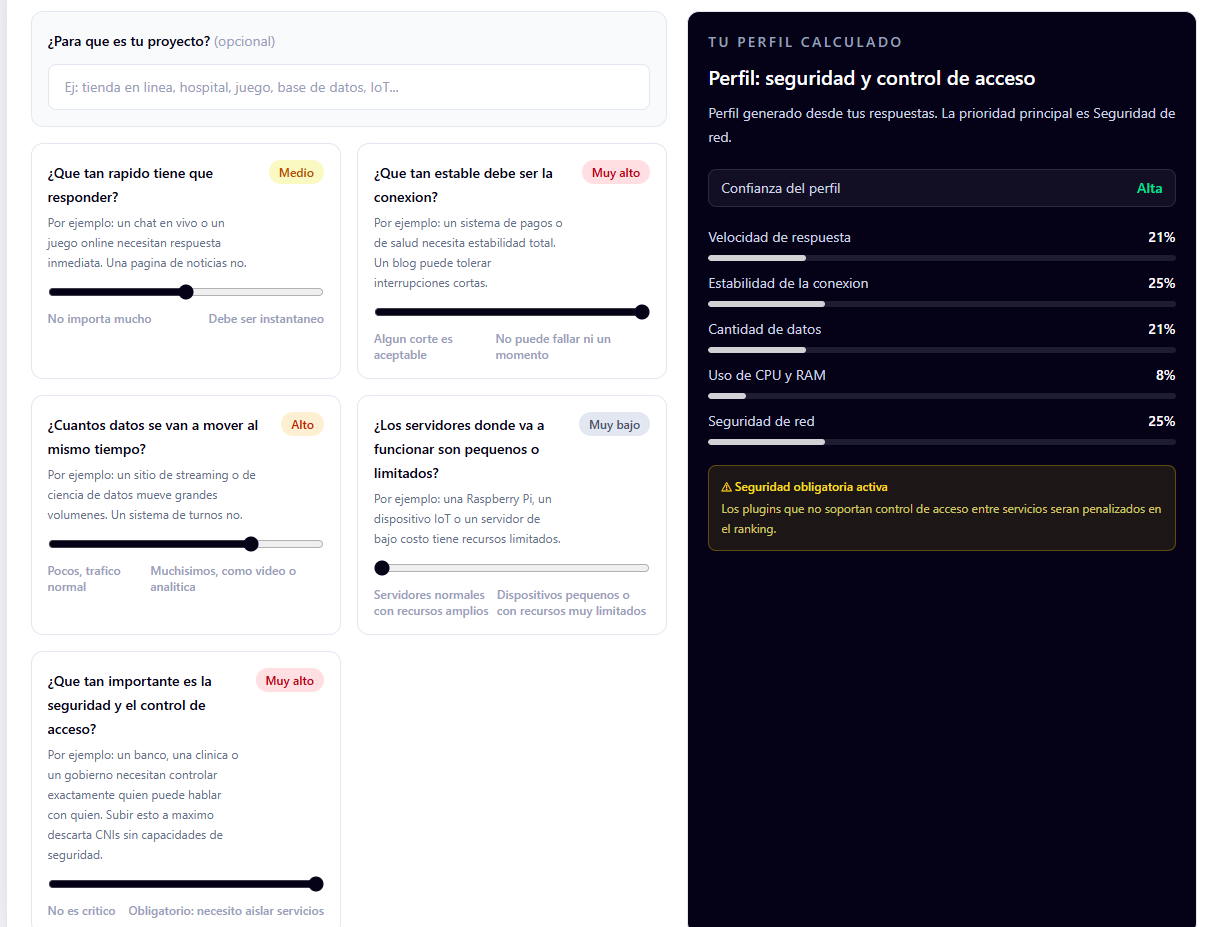
\includegraphics[width=0.85\textwidth]{figures/rec_fintech_preguntas.png}
  \caption{Configuración de sliders para el perfil Fintech / Seguridad en el Recomendador CNI.}
  \label{fig:rec_fintech_preguntas}
  \end{figure}

  \begin{figure}[htbp]
  \centering
  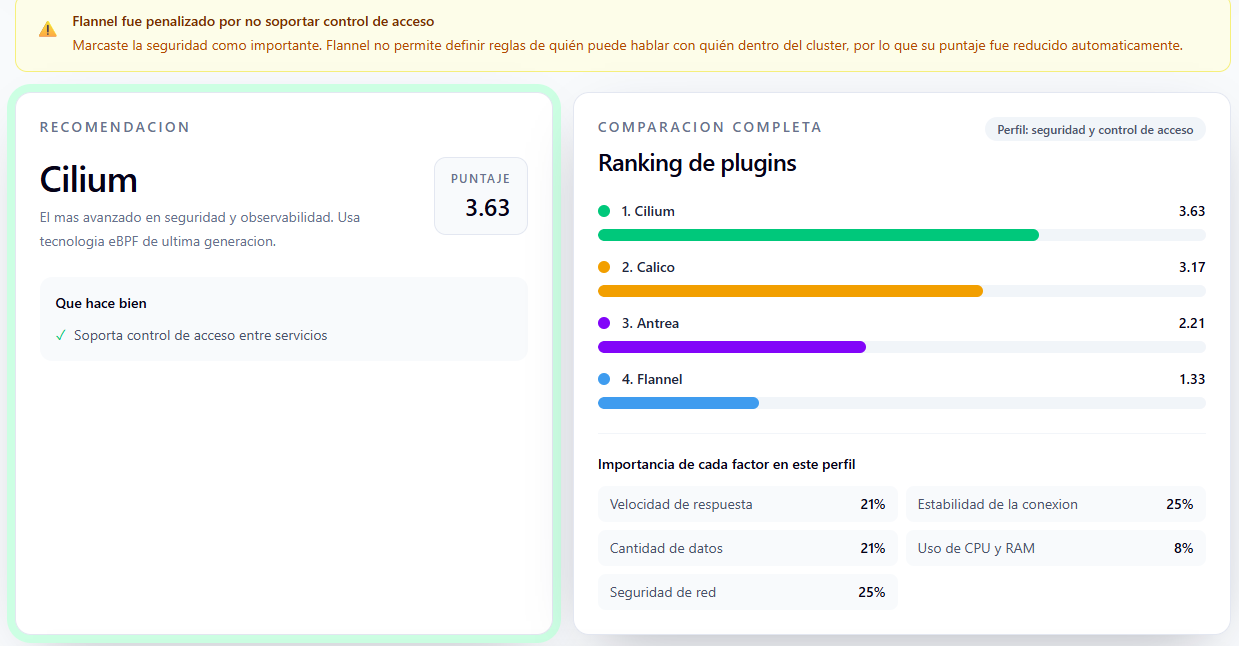
\includegraphics[width=0.95\textwidth]{figures/rec_fintech.png}
  \caption{Resultados del ranking MCDA en el prototipo interactivo para el perfil Fintech / Seguridad (Ganador: Cilium con 3.631).}
  \label{fig:rec_fintech_resultados}
  \end{figure}
  
  \item \textbf{Perfil Streaming / Rendimiento:} Flannel resulta recomendado con un puntaje de $3.686$. En el testbed, Flannel demostró un rendimiento balanceado y la estabilidad de red más alta al registrar solo 11,774 retransmisiones TCP frente a las 68,993 de Calico. Dado que la tasa de reenvío influye en la estabilidad de la transmisión de flujos continuos, la robustez de Flannel sumada a su eficiencia computacional compensa el mayor throughput bruto de Calico.
  
  \textbf{Réplica en el Recomendador SPA:} Para replicar el puntaje de $3.686$ de Flannel y $3.567$ de Calico, el usuario debe establecer las siguientes prioridades:
  \begin{itemize}
    \item Latencia: \emph{Muy Alto} ($5/5$)
    \item Estabilidad (Jitter): \emph{Alto} ($4/5$)
    \item Throughput: \emph{Muy Alto} ($5/5$)
    \item Límite de Recursos: \emph{Bajo} ($2/5$)
    \item Nivel de Seguridad: \emph{Bajo} ($2/5$)
  \end{itemize}
  Esta configuración prioriza la QoS de red cruda (throughput y latencia con pesos del $25.1\%$ y $27.7\%$ respectivamente) sin requerir seguridad restrictiva, lo que resulta en la victoria de Flannel por estabilidad.
  
  \item \textbf{Perfil IoT / Recursos limitados:} Flannel se posiciona como el CNI recomendado con $3.834$ frente a Cilium ($3.232$), Calico ($2.952$) y Antrea ($2.224$). Flannel destaca como el plugin que induce el menor estrés general bajo carga ($19.45\%$ de CPU del nodo y $1176.54$ MB de RAM global), lo cual se alinea con la prioridad de este perfil (28\% de peso a la eficiencia de recursos). Como se discute en el Capítulo~\ref{sec:Resultados}, esta métrica de RAM captura la huella del host bajo tráfico activo; un despliegue en nodos muy pequeños deberá aislar adicionalmente el consumo del binario en reposo.
  
  \textbf{Réplica en el Recomendador SPA:} Para replicar el puntaje de $3.834$ de Flannel, el usuario debe configurar los sliders con los siguientes valores:
  \begin{itemize}
    \item Latencia: \emph{Medio} ($3/5$)
    \item Estabilidad (Jitter): \emph{Medio} ($3/5$)
    \item Throughput: \emph{Medio} ($3/5$)
    \item Límite de Recursos: \emph{Muy Alto} ($5/5$)
    \item Nivel de Seguridad: \emph{Bajo} ($2/5$)
  \end{itemize}
  Esta selección asigna un $28.0\%$ de peso a la eficiencia de recursos. La Figura~\ref{fig:rec_iot_preguntas} y la Figura~\ref{fig:rec_iot_resultados} muestran respectivamente la entrada en la interfaz de usuario y el gráfico de barras resultante de la recomendación interactiva del sistema.

  \begin{figure}[htbp]
  \centering
  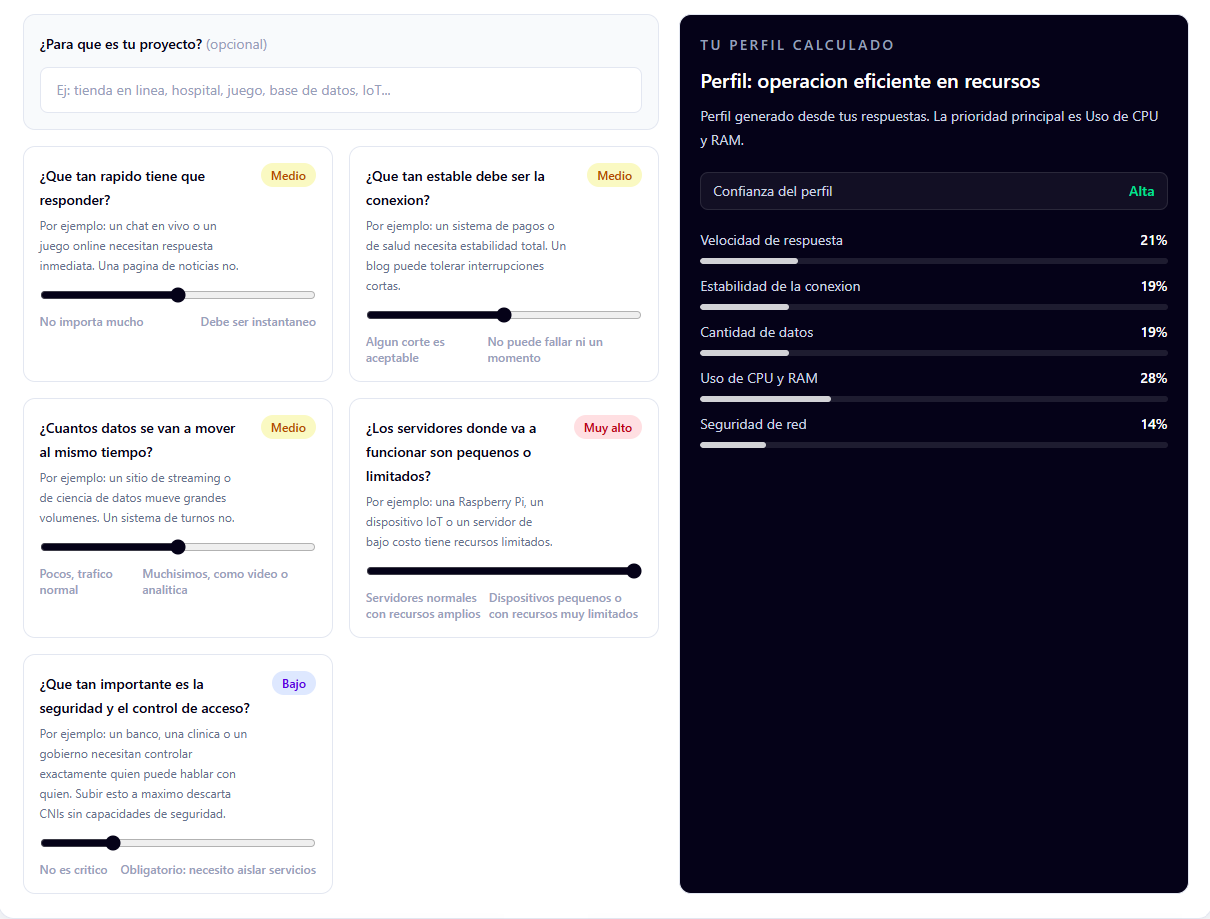
\includegraphics[width=0.85\textwidth]{figures/rec_iot_preguntas.png}
  \caption{Configuración de sliders para el perfil IoT / Recursos Limitados en el Recomendador CNI.}
  \label{fig:rec_iot_preguntas}
  \end{figure}

  \begin{figure}[htbp]
  \centering
  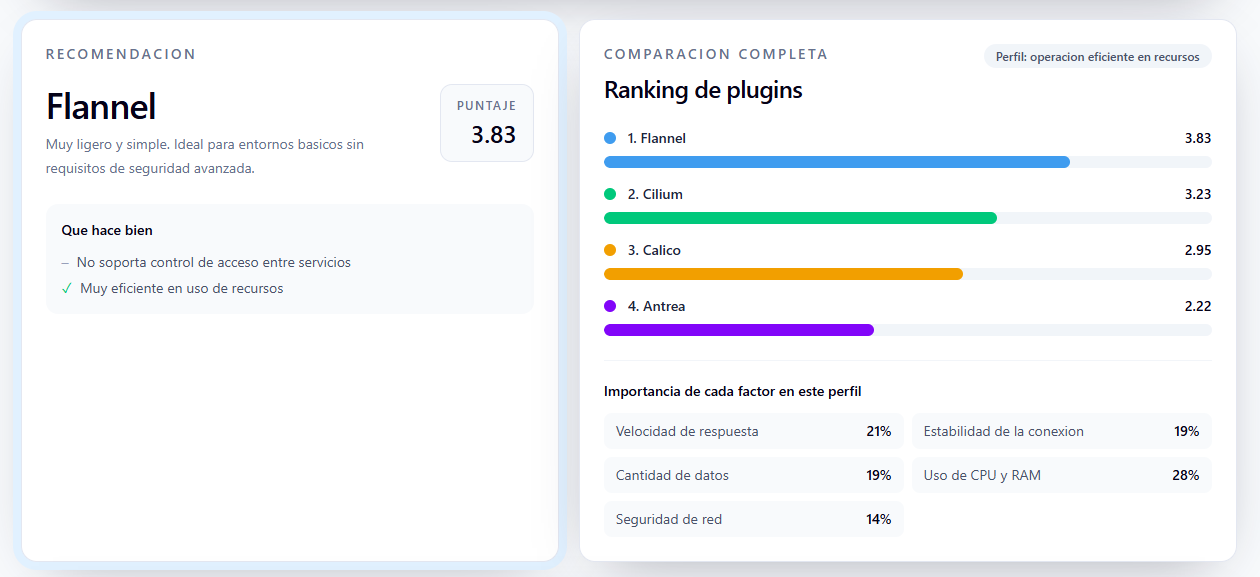
\includegraphics[width=0.95\textwidth]{figures/rec_iot.png}
  \caption{Resultados del ranking MCDA en el prototipo interactivo para el perfil IoT / Recursos Limitados (Ganador: Flannel con 3.834).}
  \label{fig:rec_iot_resultados}
  \end{figure}
\end{itemize}

\section{Lista de verificación para la configuración del recomendador CNI} \label{sec:apb_checklist}

El recomendador interactivo opera mediante cinco deslizadores de prioridad, cada uno en la escala \emph{Muy Bajo} (1) --- \emph{Bajo} (2) --- \emph{Medio} (3) --- \emph{Alto} (4) --- \emph{Muy Alto} (5). La combinación de valores genera los pesos porcentuales del modelo MCDA y, cuando la seguridad supera el nivel~4, activa la penalización no compensatoria $\times 0{,}40$ sobre plugins sin soporte de \texttt{NetworkPolicy}.

Esta lista de verificación es un instrumento cualitativo: mediante preguntas orientadas al contexto operativo del equipo, guía la asignación de cada deslizador antes de acceder al recomendador. No requiere mediciones previas; basta con que el equipo responda a cuál de las descripciones de cada fila se ajusta mejor a su caso de uso.

\begin{table}[htbp]
\centering
\scriptsize
\caption{Lista de verificación cualitativa para configurar los deslizadores del recomendador CNI.}
\label{tab:checklist_cni}
\begin{tabularx}{\textwidth}{|l|Y|Y|c|}
\hline
\textbf{Deslizador} & \textbf{Indicadores de prioridad \emph{Alta} o \emph{Muy Alta} (4--5)} & \textbf{Indicadores de prioridad \emph{Baja} o \emph{Muy Baja} (1--2)} & \textbf{Nivel elegido} \\
\hline
\textbf{Latencia}
  & APIs síncronas, portales web interactivos, bases de datos transaccionales o cualquier carga donde el usuario percibe el tiempo de respuesta individualmente.
  & Procesamiento por lotes (\emph{batch}), pipelines ETL, transferencias nocturnas o cargas donde la velocidad de respuesta por petición no es crítica.
  & \quad\quad/5 \\
\hline
\textbf{Estabilidad}
  & Transmisión de vídeo o audio en tiempo real, juegos en línea, protocolos sensibles a retransmisiones o servicios con acuerdos de nivel de servicio (SLA) de disponibilidad continua.
  & Cargas tolerantes a reintentos, transferencias de archivos grandes sin restricción de tiempo o sistemas con lógica propia de reintento a nivel de aplicación.
  & \quad\quad/5 \\
\hline
\textbf{Throughput}
  & Ingesta masiva de datos, distribución de contenido multimedia, analítica en tiempo real o cualquier carga que mueva grandes volúmenes de datos por segundo entre pods.
  & Microservicios de baja intensidad, chatbots, sistemas de notificaciones o cargas donde el número de bytes por transacción es reducido aunque el número de peticiones sea alto.
  & \quad\quad/5 \\
\hline
\textbf{Recursos}
  & Nodos con capacidad restringida (Raspberry Pi, dispositivos edge, instancias mínimas), clústeres de bajo costo o despliegues donde cada megabyte o millicore disponible importa para las cargas de trabajo.
  & Nodos de propósito general con capacidad amplia, entornos cloud elásticos o clústeres donde el CNI comparte recursos sin competencia con aplicaciones críticas.
  & \quad\quad/5 \\
\hline
\textbf{Seguridad}
  & Datos financieros, información médica o de identidad, entornos regulados (PCI-DSS, HIPAA, ISO~27001), arquitecturas Zero Trust, o cualquier clúster que aloje cargas de trabajo de distintos niveles de confianza en el mismo namespace.
  & Entornos de laboratorio, clústeres de desarrollo o pruebas aislados de internet, pipelines de CI/CD sin datos sensibles o clústeres monopropósito donde el tráfico inter-pod es homogéneo y confiable.
  & \quad\quad/5 \\
\hline
\end{tabularx}
\end{table}

\subsection*{Instrucciones de uso}

\begin{enumerate}
    \item Para cada deslizador, leer las dos columnas de indicadores y decidir cuál describe mejor el entorno operativo del clúster.
    \item Anotar el nivel elegido (1--5) en la última columna. Si el contexto queda entre ambas descripciones, usar el valor intermedio (\emph{Medio}, 3/5).
    \item Si \textbf{Seguridad} queda en nivel 4 o 5, verificar que el CNI seleccionado aplique \texttt{NetworkPolicy} en su plano de datos; de lo contrario, la penalización $\times 0{,}40$ lo descartará automáticamente.
    \item Introducir los cinco valores en el recomendador interactivo (\url{https://duwansierra.github.io/K8S-CNI-Results/}) para obtener el ranking MCDA personalizado.
    \item Comparar el resultado con los perfiles predefinidos de la Tabla~\ref{tab:apb_pesos}: si los valores elegidos se acercan a uno de los tres perfiles base (Fintech, Streaming, IoT), el recomendador producirá un ranking análogo al documentado en la Tabla~\ref{tab:apb_resultados}.
\end{enumerate}

\noindent\textbf{Nota sobre la penalización de seguridad.} Los perfiles predefinidos con nivel de seguridad 4 o 5 activan automáticamente la restricción no compensatoria: Flannel recibe el $40\%$ de su puntaje bruto, lo que lo sitúa por debajo de 2.0 en la escala 1--5 en contextos regulados, independientemente de su ventaja en recursos o estabilidad.

\section{Guía de reproducción y verificación científica} \label{sec:apb_reproducibilidad}

Para la reproducción y verificación científica paso a paso de los resultados experimentales y la compilación local del recomendador web, consulte la guía técnica detallada de comandos provista en la Sección~\ref{sec:apa_reproducibilidad} del Apéndice A.



% %%%%%%%%%%%%%%%%%%%%%%%% - ANEXO - %%%%%%%%%%%%%%%%%%%%%%%%%%
% \cleardoublepage
% \phantomsection
% \addcontentsline{toc}{chapter}{Anexos}
% \chapter*{Anexos}
% \chapter*{Anexo A}
\begin{itemize}
    \item Contiene material externo al autor, agregado como referencia o soporte

    \item No necesariamente forma parte directa del análisis principal

    \item Ejemplo: reglamentos oficiales, manuales técnicos, documentos normativos, encuestas originales
\end{itemize}



\end{document}.